\documentclass[dvipsnames]{report}
\usepackage[utf8]{inputenc}
\usepackage[dvipsnames]{xcolor}
\usepackage{tcolorbox}
\usepackage{multicol}
\usepackage{lipsum}
\usepackage[margin=0.2in]{geometry}
\usepackage{xstring}
\usepackage{xifthen}
\usepackage[dvipsnames]{xcolor}
\usepackage{setspace}
\usepackage{amsmath}
\pagenumbering{gobble}
\setlength{\columnsep}{1.5cm}
\setlength{\columnseprule}{0.2pt}
\usepackage{hyperref}
\usepackage[none]{hyphenat}
\usepackage{graphicx}
\usepackage{titlepic}
\usepackage[normalem]{ulem}
\usepackage[document]{ragged2e}
\usepackage[default]{sourcesanspro}

\hypersetup{
    colorlinks,
    citecolor=black,
    filecolor=black,
    linkcolor=black,
    urlcolor=black
}

\makeatletter
\def\@makechapterhead#1{%
  %\vspace*{5\p@}%
  {\parindent \z@ \raggedleft \normalfont
    \ifnum \c@secnumdepth >\m@ne
        \huge \bfseries \textcolor{Magenta}{#1}
        \par\nobreak
%        \vskip 10\p@
        \uwave{\hspace{\columnwidth}}%{.1pt}%
%        \vskip 10\p@
    \fi
    \interlinepenalty\@M
%    \large \bfseries \MakeUppercase{#1}\par\nobreak
%    \vskip 5\p@
  }}
\makeatother

\makeatletter
\patchcmd{\chapter}{\if@openright\cleardoublepage\else\clearpage\fi}{}{}{}
\makeatother

\newcommand{\syn}{\textbf{\textcolor{purple}{SYN}}}
\newcommand{\sab}{\textbf{\textcolor{gray}{SAB}}}
\newcommand{\com}{\textbf{\textcolor{red}{COM}}}
\newcommand{\rav}{\textbf{\textcolor{blue}{RAV}}}
\newcommand{\sen}{\textbf{\textcolor{BurntOrange}{SEN}}}
\newcommand{\med}{\textbf{\textcolor{green}{MED}}}

\newenvironment{battle}[2][]{\begin{tcolorbox}[title=\begin{center}#2 \ifthenelse{\isempty{#1}}{}{- #1}\end{center},colbacktitle=red!50!white]}{\end{tcolorbox}}

\newenvironment{shop}[1]{\begin{tcolorbox}[title=\begin{center}SHOP\, #1 GIL\end{center},colbacktitle=blue!50!white]}{\end{tcolorbox}}

\newenvironment{upgrade}{\begin{tcolorbox}[title=\begin{center}UPGRADE\end{center},colbacktitle=purple!50!white]}{\end{tcolorbox}}

\newenvironment{menu}{\begin{tcolorbox}[title=\begin{center}MENU\end{center},colbacktitle=black!50!white]}{\end{tcolorbox}}

\newcommand{\first}{1}
\newcommand{\second}{2}
\newcommand{\third}{3}
\newcommand{\fourth}{4}
\newcommand{\fifth}{5}
\newcommand{\sixth}{6}

\newcommand{\paradigm}{\item \textbf{Paradigm}}
\newcommand{\crystarium}{\item \textbf{Crystarium}}
\newcommand{\equip}{\item \textbf{Equipment}}

\newcommand{\stagger}{\textbf{STAGGER}}

\newcommand{\paradigmline}[4][]{#2 & #3 & #4 & \ifthenelse{\equal{#1}{}}{}{$\leftarrow$ \textit{Default}}}

\newcommand{\paradigmdeck}[7]{\begin{tabular}{c|c|cc} #1 \\ \cline{1-3} #2 \\ #3 \\ #4 \\ #5 \\ #6 \\ #7 \\ \end{tabular}}

\newcommand{\paradigmdeckthree}[4]{\begin{tabular}{c|c|cc} #1 \\ \cline{1-3} #2 \\ #3 \\ #4 \\ \end{tabular}}

\newcommand{\paradigmdeckfour}[5]{\begin{tabular}{c|c|cc} #1 \\ \cline{1-3} #2 \\ #3 \\ #4 \\ #5 \\  \end{tabular}}

\newcommand{\paradigmdeckfive}[6]{\begin{tabular}{c|c|cc} #1 \\ \cline{1-3} #2 \\ #3 \\ #4 \\ #5 \\ #6 \\ \end{tabular}}

\newcommand{\save}[1]{Save prompt after cut-scene \##1}

\newcommand{\pickup}[2]{Pick up the \textbf{#1} located #2.}

\newcommand{\itemdrop}[2]{#1\% chance of a \textbf{#2}}

\newcommand{\decep}[2]{\textbf{Deceptisol} on the #1, cancel on the #2.}

\setlength{\columnsep}{.5cm}

\usepackage{enumitem}
\setitemize{noitemsep,topsep=0pt,parsep=0pt,partopsep=0pt}
\usepackage{graphicx}
\ifthenelse{\equal{\platformtype}{pc}}
{
	\ifthenelse{\equal{\notetype}{snow_turtle}}
	{
		\title{FF13 Any\%}
	}
	{
		\title{FF13 Any\% - Lightning}
	}
}
{
	\title{FF13 Any\% - Console}
}

\author{Mr.Tyton}
\titlepic{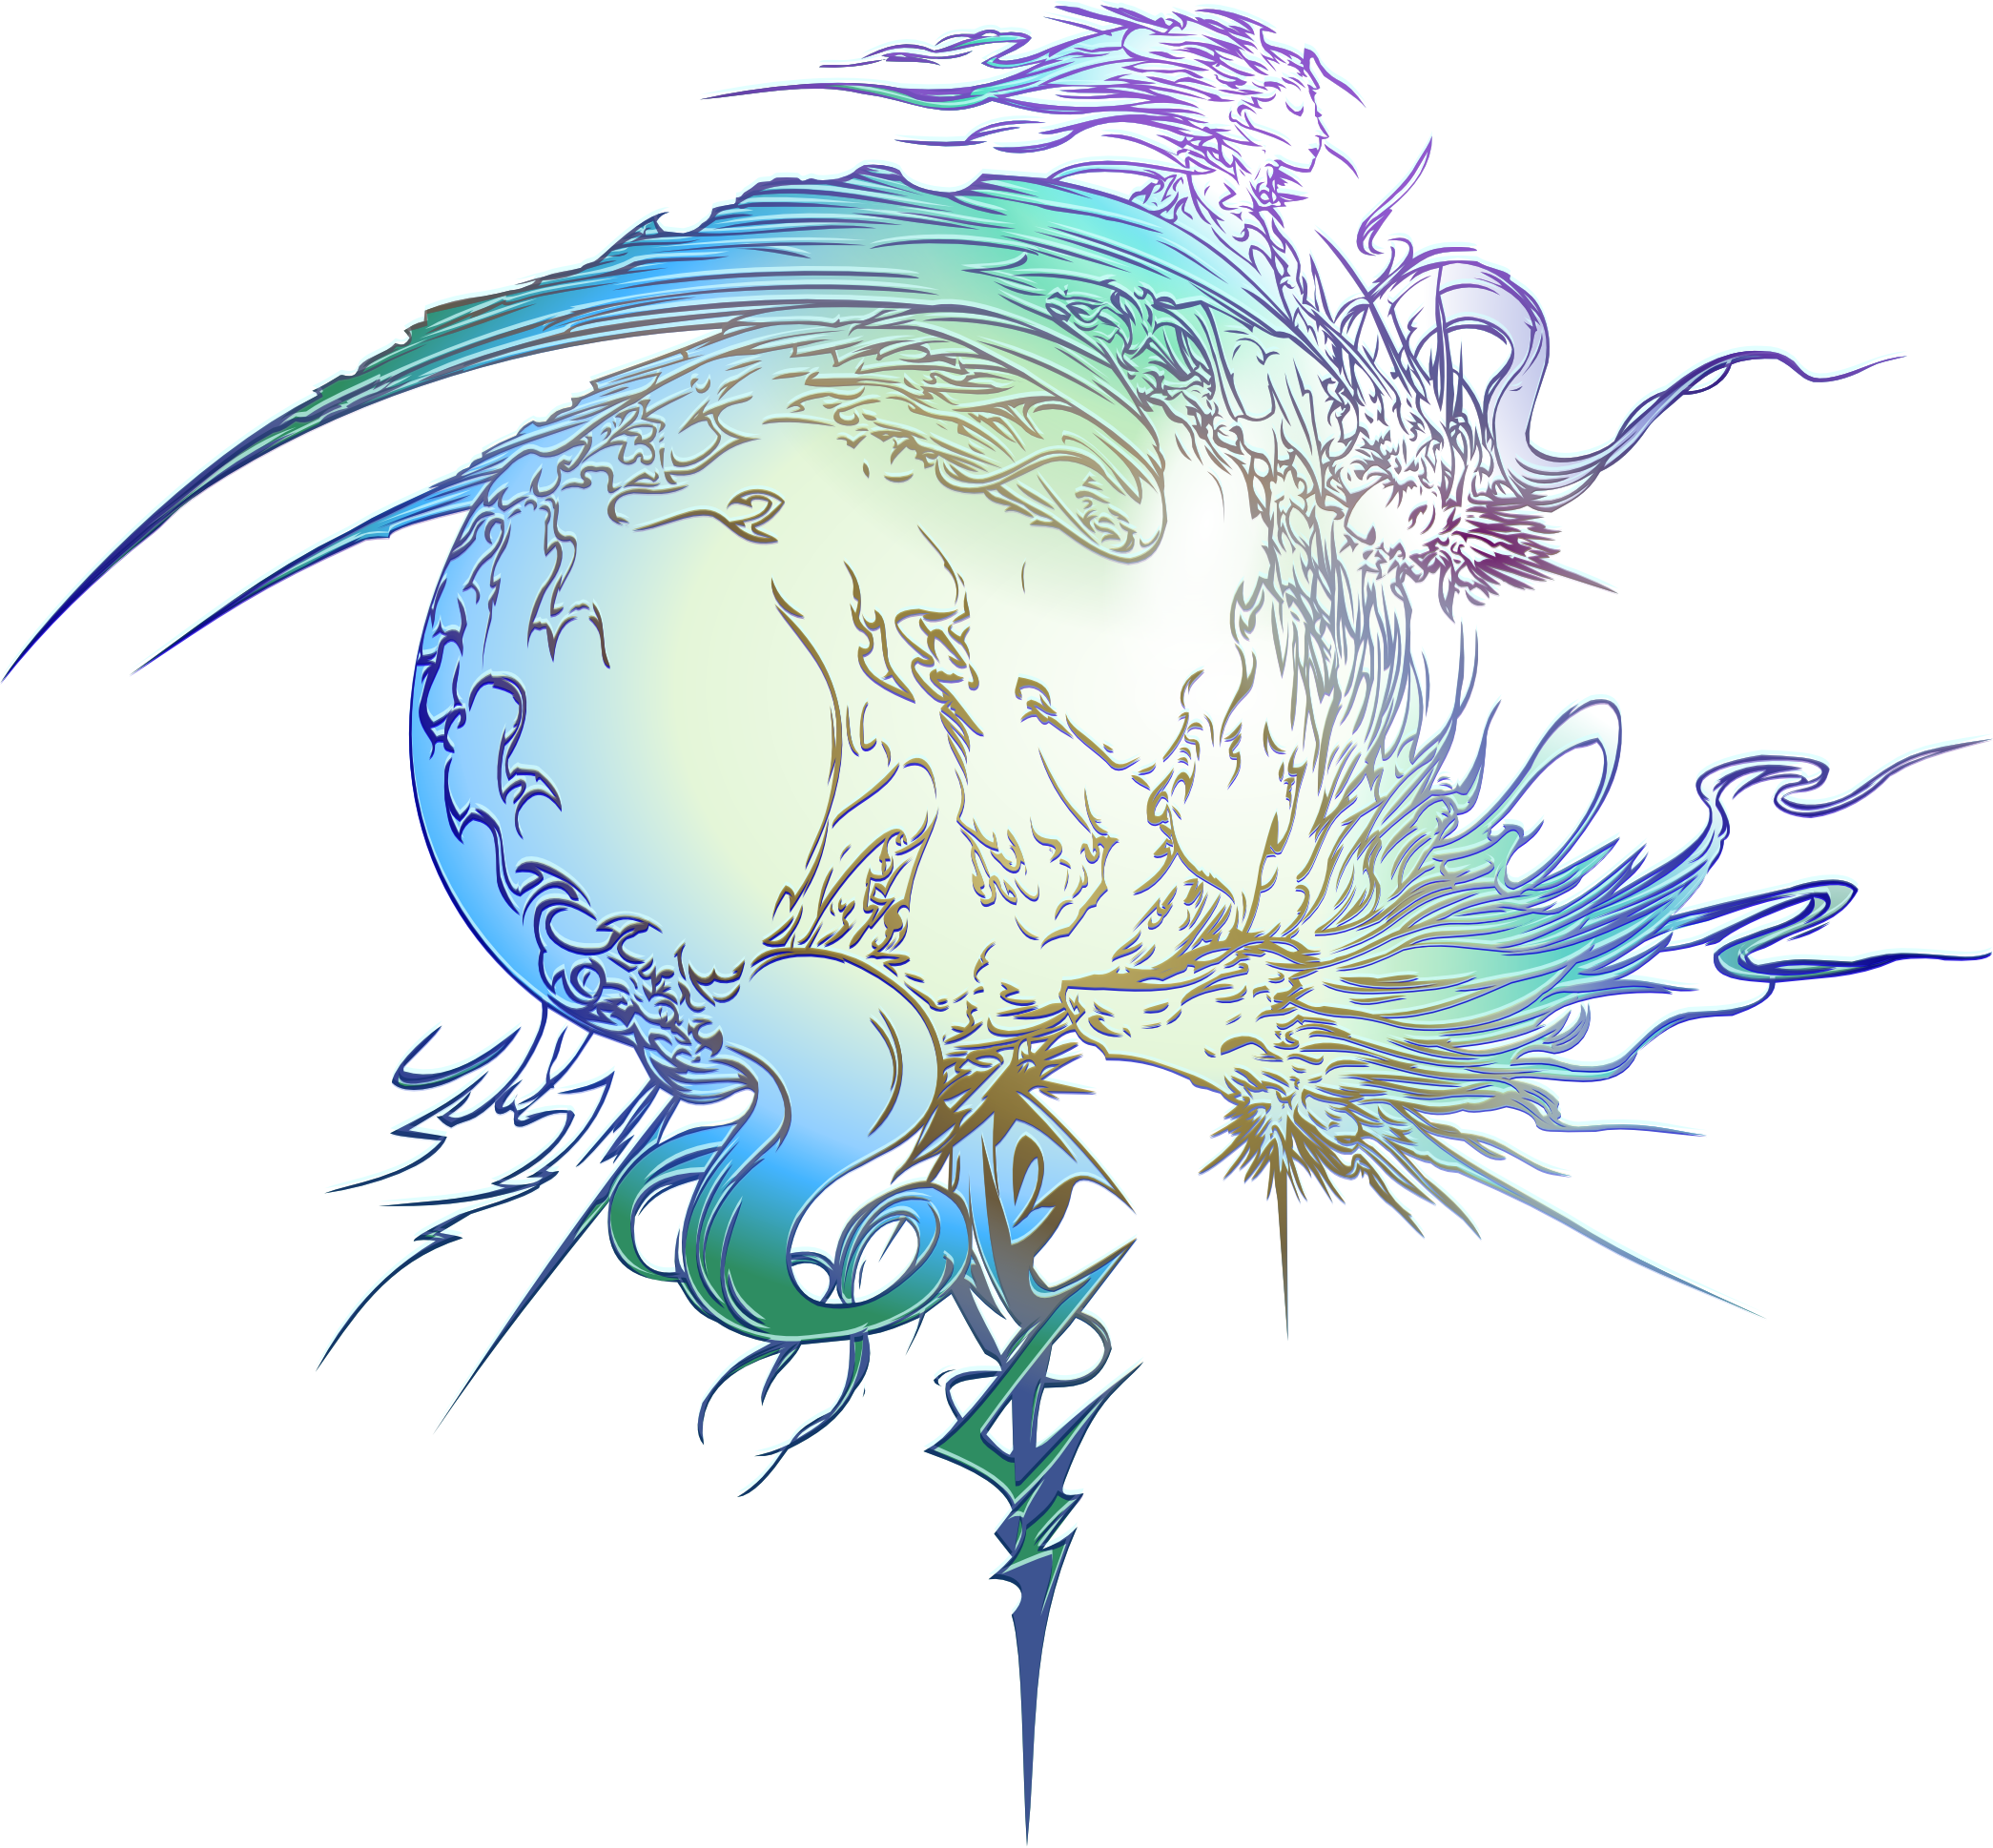
\includegraphics[width=\textwidth]{final_fantasy_xiii_logo_by_eldi13_d42h0oc}}
\begin{document}
\singlespacing
\maketitle
\tableofcontents


\section*{Acknowledgements}
Everyone in the FF13 Discord. In no particular order: \textbf{Roosta}, \textbf{LogicDolphin}, \textbf{Flux}, \textbf{Yeswally1}, \textbf{LilSharkie}, \textbf{xJakeDreamer}, \textbf{TehMonkey\_},  \textbf{xP3ndulum},  \textbf{NijiBashira}, \textbf{Mrzwanzig}, \textbf{QazPlm9000}, \textbf{Hoishin}, \textbf{tiornys}, \textbf{MLSTRM}, \textbf{Kayarune} and anyone else I forgot.

\newpage

\begin{multicols*}{2}
\chapter[Chapter 1]{}
\begin{multicols}{2}
\begin{battle}{Manasvin Warmech (1)}
\end{battle}

Camera Trick for the first dodge, stick by the right for the second.

\begin{battle}{Pantheron \& PSICOM Warden}
\end{battle}

Camera Trick on the ramp and hope Sazh is nice.

\begin{battle}{PSICOM Marauder \& PSICOM Enforcer x2}
\itemdrop{19}{Phoenix Down}
\end{battle}

Legendary Dodge - Camera trick immediately. Hopefully the dogs hold short and you can run to the right around them.

\begin{battle}{Legendary Dodge - Pantheron x2 \& PSICOM Warden x2}
\begin{itemize}
    \item Hand Grenade PSICOM Warden A
    \item Repeat PSICOM Warden B
    \item Repeat Pantheron A
    \item Hand Grenade + Auto Battle if anyone is left alive
\end{itemize}

\itemdrop{19}{Phoenix Down}
\end{battle}

Camera trick after the first dodge in the Beta Behemoth hallway.

\begin{battle}{Beta Behemoth}
\begin{itemize}
    \item Throw a potion to prevent Snow's interruption by the swipe.
    \item Auto-battle twice
    \item Auto-battle and execute at 1.5 ATB, should dodge swipe
    \item Auto-battle twice
    \item Auto-battle, execute at 1.9 ATB, should dodge swipe
    \item Auto-battle until victory
\end{itemize}
\end{battle}

\save{1}

\begin{battle}{Myrmidon}
\begin{itemize}
    \item Auto battle and execute at 1.5 ATB
    \item Auto-battle
    \item Auto-battle 1 Attack
    \item Auto-battle and execute at 1.5 ATB
    \item Auto-battle
    \item Throw a potion at any point if anyone goes to less than 60hp
    \item Auto-battle once staggered, try to interrupt.
\end{itemize}

\itemdrop{25}{Polymer Emulsion}
\end{battle}

\pickup{Power Circle}{in front}

\begin{menu}
\begin{itemize}
    \item \textbf{Equipment}
    \begin{itemize}
        \item Snow
        \begin{itemize}
            \item Optimize: Offensive (Power Circle)
        \end{itemize}
    \end{itemize}
\end{itemize}
\end{menu}

Run through and fight if you fail it.

\begin{battle}{Pantheron x2 \& PSICOM Aerial Recon x3}
\begin{itemize}
    \item Hand Grenade whatever PSICOM Aerial Recon will hit the most things. Swap targets after every one to change Gadot's damage.
    \item Hand Grenades until the last thing left is not at full hp.
\end{itemize}

\itemdrop{27.1}{Phoenix Down}
\end{battle}

\begin{battle}{PSICOM Warden \& PSICOM Enforcer x2}
\itemdrop{27.1}{Phoenix Down}
\end{battle}

\save{1}
\end{multicols}


\chapter[Chapter 2]{}

\begin{multicols}{2}
\begin{battle}{Pantheron}
\begin{itemize}
    \item Attack x2
    \item Repeat
\end{itemize}
\end{battle}

\begin{menu}
\begin{itemize}
    \item \textbf{Settings}
    \begin{itemize}
        \item Battle Speed: Slow
    \end{itemize}
\end{itemize}
\end{menu}

Farm both 100\% Deceptisols by waiting 23 seconds.
\begin{battle}{Zwerg Scandroid x3 (1)}
\itemdrop{100}{Deceptisol}
\end{battle}

\begin{battle}{Zwerg Scandroid x3 (2)}
\itemdrop{100}{Deceptisol}
\end{battle}

\begin{menu}
\begin{itemize}
    \item \textbf{Settings}
    \begin{itemize}
        \item Battle Speed: Normal
    \end{itemize}
\end{itemize}
\end{menu}

\begin{battle}{Pantheron x2}
\begin{itemize}
    \item Hand Grenade x3, Attack x2 if not dead
    \item Each time, Target Pantheron A while ATB is charging, then switch to Pantheron B for Grenade
\end{itemize}
\itemdrop{12}{Fortisol}
\end{battle}

Camera trick the dogs after prompt.

\begin{battle}{Zwerg Scandroid x4 (Lightning Lead)}
\begin{itemize}
    \item Attack after 32 seconds have passed. Should be when Sazh attacks the last one remaining, also go by audio cue.
\end{itemize}
\itemdrop{96}{Deceptisol} if got the 0 stars
\end{battle}

\pickup{Phoenix Down}{after the scandroids}

\begin{battle}{Pantheron \& Zwerg Scandroid x2 (Lighting Lead)}
\itemdrop{12}{Fortisol}
\end{battle}

\pickup{Gladius}{after the Pantheron}

\begin{menu}
\begin{itemize}
    \item \textbf{Equipment}
    \begin{itemize}
        \item Lightning
        \begin{itemize}
            \item Optimize: Offensive (Gladius)
        \end{itemize}
    \end{itemize}
\end{itemize}
\end{menu}

\begin{battle}{Pantheron \& Zwerg Scandroid x2 (Snow Lead)}
\itemdrop{12}{Deceptisol}
\end{battle}
Access the menu in mid-air.

\begin{menu}
\begin{itemize}
    \item \textbf{Settings}
    \begin{itemize}
        \item Battle Speed: Slow
    \end{itemize}
\end{itemize}
\end{menu}

\begin{battle}{Zwerg Scandroid x4 (Vanille Lead) \textbf{Don't Pre-Empt}}
\begin{itemize}
    \item Auto-battle 1 Attack
    \item Wait 32 seconds to end or let Hope end the fight.
\end{itemize}
\itemdrop{96}{Fortisol}
\end{battle}

\pickup{Fortisol}{beind the Scandroids}
\begin{menu}
\begin{itemize}
    \item \textbf{Settings}
    \begin{itemize}
        \item Battle Speed: Normal
    \end{itemize}
\end{itemize}
\end{menu}

\begin{battle}{Ghoul x3}
\itemdrop{12}{Fortisol}
\end{battle}

Check shrouds. Minimum required 2 Deceptisols/Fortisols, safety is 4 Deceptisols/3 Fortisols.

Ghoul hallway is as follows: {\bf Fortisol, Deceptisol, Deceptisol, Fortisol, Deceptisol}

\begin{battle}{Ghoul}
\begin{itemize}
    \item Wait 41 seconds before attacking or let Sazh finish the battle.
\end{itemize}
\end{battle}

\textbf{Fortisol} on the elevator.

\begin{battle}{Anima}

\begin{itemize}
    \item Blitz Anima while dodging his swipes until the Left Manipulator dies
    \item Potion if anyone is below 100 HP
    \item Attack Anima until half health while still dodging his swipes
    \item Kill the Right Manipulator
    \item Auto-battle until victory.
\end{itemize}
\end{battle}

\save{2}

\save{3}

\end{multicols}


\chapter[Chapter 3]{}

\renewcommand{\first}{[1] - Relentless Assault (\com/\rav/\rav)}
\begin{multicols}{2}

\begin{battle}{Ghast x3}
\begin{itemize}
    \item \first
    \begin{itemize}
        \item Skip Tutorial, Auto-battle a Ghast that isn't the default
        \item Select Attack x3, change target and execute when Snow starts to attack
        \item Repeat 1 Attack on the surviving Ghast
    \end{itemize}
\end{itemize}
\itemdrop{8}{Deceptisol}
\end{battle}
\begin{menu}
\begin{itemize}
    \item \textbf{Equipment}
    \begin{itemize}
        \item Snow
        \begin{itemize}
            \item Equip: Wild Bear
        \end{itemize}
    \end{itemize}
\end{itemize}
\end{menu}
\begin{shop}{3\,000}
\begin{itemize}
    \item B\&W Outfitters
    \begin{itemize}
        \item Sell
        \begin{itemize}
        \item Items
        \begin{itemize}
            \item Phoenix Down x2
        \end{itemize}
         \item Weapons
        \begin{itemize}
            \item Power Circle
        \end{itemize}
        \item \textit{If still not enough Gil:}
	        \item Components
	        \begin{itemize}
		        \item Credit Chip
	        \end{itemize}
        \end{itemize}
        \item Buy
        \begin{itemize}
            \item Power Wristband
            \item Magician's Mark x2
        \end{itemize}
    \end{itemize}
\end{itemize}
\end{shop}
\begin{menu}
\begin{itemize}
    \item \textbf{Paradigms}
    \begin{itemize}
        \item \paradigmdeckfour{%
\paradigmline{Lightning}{Snow}{Vanille}}%
{\paradigmline{(\rav)}{\rav}{\rav}}%
{\paradigmline{\com}{\sen}{\med}}%
{\paradigmline[3]{\textit{[\com]}}{\textit{\com}}{\textit{\rav}}}%
{\paradigmline{[\com]}{\com}{\rav}}
    \end{itemize}
    \item \textbf{Crystarium}
    \begin{itemize}
        \item Lightning
        \begin{itemize}
            \item Commando
            \begin{itemize}
                \item 1 node, Strength +4
            \end{itemize}
        \end{itemize}
        \item Snow
        \begin{itemize}
            \item Commando
            \begin{itemize}
                \item Both side nodes, Strength +18, HP +70
            \end{itemize}
        \end{itemize}
    \end{itemize}
    
    \item \textbf{Equipment}
    \begin{itemize}
        \item Lightning
        \begin{itemize}
            \item Optimize: Offensive (Power Wristband)
        \end{itemize}
        \item Vanille ($\rightarrow \rightarrow$)
        \begin{itemize}
            \item Optimize: Offensive (Magician's Mark)
        \end{itemize}
        \item Sazh ($\rightarrow$)
        \begin{itemize}
            \item Optimize: Offensive (Magician's Mark)
        \end{itemize}
    \end{itemize}
\end{itemize}
\end{menu}
\renewcommand{\first}{[1] Tri-Disaster (\rav/\rav/\rav)}

\renewcommand{\second}{[2] Solidarity (\com/\sen/\med)}

\renewcommand{\third}{[3] Aggression (\com/\com/\rav)}

\renewcommand{\fourth}{[4] Aggression (\com/\com/\rav)}

\begin{battle}{PSICOM Warden x7}
\itemdrop{8}{Fortisol} \itemdrop{52.2}{Phoenix Down}
\end{battle}
\vfill
\columnbreak
Start walking backwards once you cross the line in the center of the bridge, Snow will start talking and it makes the cut-scene happen faster.

\begin{battle}{Manasvin Warmech (2)}
\begin{itemize}
    \item \third
    \begin{itemize}
        \item Libra
        \item Auto-battle, shift when Lightning executes the third attack or gets hit
    \end{itemize}
    \item \fourth
    \begin{itemize}
        \item Auto-battle
        \item Shift after Vanille's third aero
    \end{itemize}
    \item \first
    \begin{itemize}
        \item Potion if Lightning has less than 120 hp
        \item Auto-chain, execute when Crystal Rain text appears on screen.
        \item \textbf{STAGGER}
        \item Shift after Vanille's third aero
    \end{itemize}
    \item \third
    \begin{itemize}
        \item Auto-battle
        \item Shift after Vanille's third aero
    \end{itemize}
    \item \second
    \begin{itemize}
        \item Shift after Provoke
    \end{itemize}
    \item \third
    \begin{itemize}
    	\item Auto-battle
    	\item Shift after Snow's or Lightning's third attack, whichever happens last
    \end{itemize}
    \item \fourth
    \begin{itemize}
        \item Auto-battle 2 Attacks
        \item Auto-battle twice
    \end{itemize}
    \item \third
    \begin{itemize}
        \item Auto-battle
        \item Auto-battle 1 Attack if survived
    \end{itemize}
\itemdrop{8}{Deceptisol}
\end{itemize}
\end{battle}

\begin{menu}
\begin{itemize}
    \item \textbf{Paradigms}
    \begin{itemize}
        \item \paradigmdeckfive{%
        \paradigmline{Lightning}{Vanille}{Sazh}}%
{\paradigmline[1]{\textit{\com}}{\textit{\rav}}{\textit{\rav}}}%
{\paradigmline{\com}{\med}{\rav}}%
{\paradigmline{[\rav]}{\rav}{\rav}}%
{\paradigmline{[\rav]}{\rav}{\rav}}%
{\paradigmline{[\com]}{\rav}{\rav}}
    \end{itemize}
    \item \textbf{Crystarium}
    \begin{itemize}
        \item Vanille
        \begin{itemize}
            \item Ravager
            \begin{itemize}
                \item 2 nodes, Water
            \end{itemize}
        \end{itemize}
    \end{itemize}
\end{itemize}
\end{menu}

\renewcommand{\first}{[1] Relentless Assault (\com/\rav/\rav)}
\renewcommand{\second}{[2] Diversity (\com/\med/\rav)}
\renewcommand{\third}{[3] Tri-Disaster (\rav/\rav/\rav)}
\renewcommand{\fourth}{[4] Tri-Disaster (\rav/\rav/\rav)}
\renewcommand{\fifth}{[5] Relentless Assault (\com/\rav/\rav)}

\decep{brog fridge}{frogs}
\vfill

\begin{battle}{Alpha Behemoth}
\begin{itemize}
    \item \first
    \begin{itemize}
        \item Auto-battle
        \item Shift after swipe connects
    \end{itemize}
    \item \third
    \begin{itemize}
        \item Auto-chain
        \item Libra
        \item Auto-chain 2 Thunders, refresh Sazh
    \end{itemize}
    \item \fourth
    \begin{itemize}
        \item Auto-chain
        \item Shift after Vanille's third Water
    \end{itemize}
    \item \first
    \begin{itemize}
        \item Attack x3
        \item \textbf{STAGGER}. Try to time shfit so that it happens during this animation.
    \end{itemize}
    \item \fifth
    \begin{itemize}
        \item Repeat until victory.
    \end{itemize}
\end{itemize}
\itemdrop{8}{Deceptisol}
\end{battle}

\decep{3 sentry bots}{3 soldiers}

\decep{final jump}{3 sentries after the cut-scene}

\pickup{Phoenix Down}{right of the stairs if you have none or for money safety} \pickup{2 Librascopes}{left of the stairs}
\vfill

\begin{battle}{Garuda Interceptor}
\begin{itemize}
    \item \first
    \begin{itemize}
        \item Attack x3
        \item Shift mid-air
    \end{itemize}
    \item \fifth
    \begin{itemize}
        \item Libra
        \item \stagger
        \item Repeat
        \item Attack x2
    \end{itemize}
    \item \first
    \begin{itemize}
        \item Repeat
        \item Skip 2 cutscenes
        \item Attack x3
        \item Shift mid-air
    \end{itemize}
    \item \third
    \begin{itemize}
        \item Auto-chain
    \end{itemize}
    \item \fourth
    \begin{itemize}
        \item Auto-chain
        \item Shift after either Vanille's third Aero or after Sazh's third Fire, whichever is first
    \end{itemize}
    \item \third
    \begin{itemize}
        \item Auto-chain twice
    \end{itemize}
    \item \first
    \begin{itemize}
        \item \stagger
        \item Repeat until victory, ATB refresh with [5]
    \end{itemize}
\end{itemize}
\itemdrop{8}{Fortisol}
\end{battle}

\save{1}
\end{multicols}

\renewcommand{\first}{[1] Commando (\com)}
\renewcommand{\second}{[2] Sentinel (\sen)}
\renewcommand{\third}{[3] Ravager (\rav)}

\begin{battle}{PSICOM Ranger x3\, Stiria \& Nix}
\begin{itemize}
    \item \first
    \begin{itemize}
        \item Attack x3 PSICOM Ranger C
        \item Repeat on whichever Ranger is at full hp (can refresh between [2] and [1] for tiny save)
    \end{itemize}
    \item Skip cutscene
    \item \first
    \begin{itemize}
        \item Attack-Ruin-Attack
    \end{itemize}
    \item \third
    \begin{itemize}
        \item Froststrike x3
        \item Repeat 2 Froststrikes
    \end{itemize}
    \item \second
    \begin{itemize}
        \item Shift after ATB Charge attacks end
    \end{itemize}
    \item \first
    \begin{itemize}
        \item Repeat. If interrupted, cancel and repeat again.
    \end{itemize}
    \item \third
    \begin{itemize}
        \item Repeat
        \item Repeat one Froststrike
    \end{itemize}
    \item Repeat between [1] and [3] until ATB Charge attacks, then switch to [2]
    \item X when Gestalt fills, Select skips animation
\end{itemize}
\itemdrop{8}{Fortisol} \itemdrop{27.1}{Phoenix Down}
\end{battle}


\chapter[Chapter 4]{}
\begin{paracol}{2}
	\renewcommand{\first}{[1] Relentless Assault (\com/\rav/\rav)}

	\begin{battle}{Pantheron x4}
		\begin{itemize}
			\item \first
			      \begin{itemize}
				      \item Blitz Pantheron C ($\leftarrow$)
				      \item Auto-battle Pantheron A
			      \end{itemize}
		\end{itemize}
		\itemdrop{6}{Fortisol}
	\end{battle}

	\decep{last jump}{Pulsework Soldier}
	\switchcolumn
	\renewcommand{\first}{[1] Relentless Assault (\com/\rav/\rav)}

	\begin{battle}{Pantheron x4}
		\begin{itemize}
			\item \first
			      \begin{itemize}
				      \item Blitz Pantheron C
				      \item Attack x3 Pantheron A
			      \end{itemize}
		\end{itemize}
		\itemdrop{6}{Fortisol}
	\end{battle}

	\decep{last jump}{Pulsework Soldier}
	\switchcolumn*

	\begin{menu}
		\begin{itemize}
			\item \textbf{Paradigms}
			      \begin{itemize}
				      \item \paradigmdeckfive{%
					            \paradigmline{Sazh}{Vanille}{}}%
				            {\paradigmline{\rav}{\rav}{}}%
				            {\paradigmline{\syn}{\sab}{}}%
				            {\paradigmline{\rav}{\med}{}}%
				            {\paradigmline[4]{\textit{\rav}}{\textit{[\sab]}}{}}%
				            {\paradigmline{[\rav]}{\rav}{}}
			      \end{itemize}


		\end{itemize}
	\end{menu}
	\switchcolumn
	\begin{menu}
		\begin{itemize}
			\item \textbf{Paradigms}
			      \begin{itemize}
				      \item \paradigmdeckfive{%
					            \paradigmline{Sazh}{Vanille}{}}%
				            {\paradigmline{\rav}{\rav}{}}%
				            {\paradigmline{\syn}{\sab}{}}%
				            {\paradigmline{\rav}{\med}{}}%
				            {\paradigmline[4]{\textit{\rav}}{\textit{[\sab]}}{}}%
				            {\paradigmline{[\rav]}{\rav}{}}
			      \end{itemize}
			\item \textbf{Crystarium}
			      \begin{itemize}
				      \item Vanille
				            \begin{itemize}
					            \item Ravager
					                  \begin{itemize}
						                  \item 2 nodes, Water
					                  \end{itemize}
				            \end{itemize}
			      \end{itemize}
		\end{itemize}
	\end{menu}
	\switchcolumn*
	\renewcommand{\first}{[1] Dualcasting (\rav/\rav)}
	\renewcommand{\second}{[2] Tide Turner (\syn/\sab)}
	\renewcommand{\third}{[3] Yin \& Yang (\rav/\med)}
	\renewcommand{\fourth}{[4] Undermine (\rav/\sab)}
	\renewcommand{\fifth}{[5] Dualcasting (\rav/\rav)}
	\begin{battle}{Pulsework Solider \& Watchdrone x3}
		\begin{itemize}
			\item \fourth
			      \begin{itemize}
				      \item Select Libra, hover over Pulsework Soldier ($\downarrow$); Libra on Watchdrone C after Vanille starts casting
				      \item Auto-chain and shift after Sazh's third fire
			      \end{itemize}
			\item \second
			      \begin{itemize}
				      \item Auto-support twice (Vanille then Sazh)
				      \item Shift after Vanille's string
			      \end{itemize}
			\item \textit{If Pulsework Soldier staggered with Vanille's first cast}
			      \begin{itemize}
				      \item \first
				            \begin{itemize}
					            \item Auto-chain 2 fires
					            \item Shift after Vanille finishes
				            \end{itemize}
				      \item \fifth
				            \begin{itemize}
					            \item Auto-chain
					            \item When the second Watchdrone will die to Vanille, let her start the chain and then Auto-chain the Soldier
					            \item ATB refresh with [1]
				            \end{itemize}
			      \end{itemize}
			\item \textit{Else if it staggered with the second cast}
			      \begin{itemize}
				      \item \first
				            \begin{itemize}
					            \item After Vanille starts casting, Auto-chain the Pulsework Soldier
					            \item ATB refresh with [5]
				            \end{itemize}
			      \end{itemize}
		\end{itemize}
		\itemdrop{6}{Aegisol}
	\end{battle}
	\switchcolumn
	\begin{battle}{Pulsework Solider \& Watchdrone x3}
		\begin{itemize}
			\item \fourth
			      \begin{itemize}
				      \item Select Libra, hover over Pulsework Soldier ($\leftarrow\leftarrow$); Libra on Watchdrone C after Vanille starts casting
				      \item Auto-chain and shift after Sazh's third fire
			      \end{itemize}
			\item \second
			      \begin{itemize}
				      \item Auto-support twice (Vanille first, Sazh second)
				      \item Shift after Vanille's string
			      \end{itemize}
			\item \textit{If Pulsework Soldier staggered with Vanille's first cast}
			      \begin{itemize}
				      \item \first
				            \begin{itemize}
					            \item Auto-chain 2 fires
					            \item Shift after Vanille finishes
				            \end{itemize}
				      \item \fifth
				            \begin{itemize}
					            \item Auto-chain
					            \item When the second Watchdrone will die to Vanille, let her start the chain and then Auto-chain the Soldier
					            \item ATB refresh with [1]
				            \end{itemize}
			      \end{itemize}
			\item \textit{Else if it staggered with the second cast}
			      \begin{itemize}
				      \item \first
				            \begin{itemize}
					            \item After Vanille starts casting, Auto-chain the Pulsework Soldier
					            \item ATB refresh with [1]
				            \end{itemize}
			      \end{itemize}
		\end{itemize}
		\itemdrop{6}{Aegisol}
	\end{battle}
	\renewcommand{\first}{[1] Tri-disaster (\rav/\rav/\rav)}
	\renewcommand{\fourth}{[4] Variety (\rav/\sab/\med)}
	\switchcolumn*
	\begin{battle}{Pulsework Soldier Pre-Empt}
		\begin{itemize}
			\item \first
			      \begin{itemize}
				      \item Auto-chain
				      \item \stagger, shift after Vanille's string
			      \end{itemize}
			\item \fourth
			      \begin{itemize}
				      \item Shift immediately. Vanille should be casting Deshell
			      \end{itemize}
			\item \first
			      \begin{itemize}
				      \item Auto-chain
				      \item Auto-chain 2 Fires
			      \end{itemize}
		\end{itemize}
		\itemdrop{6}{Aegisol}
	\end{battle}
	\pickup{Ninurta}{behind the Pulsework Soldier}
	\switchcolumn
	\begin{battle}{Pulsework Soldier Pre-Empt}
		\begin{itemize}
			\item \first
			      \begin{itemize}
				      \item Auto-chain
				      \item \stagger
			      \end{itemize}
			\item \fourth
			      \begin{itemize}
				      \item Immediately shift. Vanille should be casting Deshell
			      \end{itemize}
			\item \first
			      \begin{itemize}
				      \item Auto-chain twice
			      \end{itemize}
		\end{itemize}
		\itemdrop{6}{Aegisol}
	\end{battle}

	\pickup{Ninurta}{behind the Pulsework Soldier}

	\renewcommand{\first}{[1] Relentless Assault (\rav/\com/\rav)}
	\renewcommand{\second}{[2] Bully (\syn/\com/\sab)}
	\renewcommand{\third}{[3] Relentless Assault (\rav/\com/\rav)}
	\renewcommand{\fourth}{[4] Smart Bomb (\rav/\rav/\sab)}
	\renewcommand{\fifth}{[5] Tri-Disaster (\rav/\rav/\rav)}
	\renewcommand{\sixth}{[6] Malevolence (\syn/\rav/\rav)}
	\switchcolumn*
	\begin{menu}
		\begin{itemize}
			\paradigm
			\begin{itemize}
				\item \paradigmdeck{%
					      \paradigmline{Sazh}{Lightning}{Vanille}}%
				      {\paradigmline{\rav}{\com}{\rav}}%
				      {\paradigmline{\syn}{\com}{\sab}}%
				      {\paradigmline{\rav}{\com}{(\rav)}}%
				      {\paradigmline[4]{\textit{\rav}}{\textit{\rav}}{\textit{\sab}}}%
				      {\paradigmline{\rav}{[\rav]}{\rav}}%
				      {\paradigmline{[\syn]}{[\rav]}{\rav}}
			\end{itemize}

			\crystarium
			\begin{itemize}
				\item Sazh
				      \begin{itemize}
					      \item Synergist
					            \begin{itemize}
						            \item 6 Nodes, All of them
					            \end{itemize}
				      \end{itemize}
				\item Lightning
				      \begin{itemize}
					      \item Commando
					            \begin{itemize}
						            \item 2 nodes, Powerchain
					            \end{itemize}
					      \item Ravager
					            \begin{itemize}
						            \item 3 nodes, 1 Up, Strength +10
						            \item 2 nodes, HP +15 after Water
					            \end{itemize}
				      \end{itemize}
				\item Vanille
				      \begin{itemize}
					      \item Saboteur
					            \begin{itemize}
						            \item 5 nodes, Magic +4
					            \end{itemize}
				      \end{itemize}
				\item Hope
				      \begin{itemize}
					      \item Ravager
					            \begin{itemize}
						            \item 2 nodes, HP +20
					            \end{itemize}
				      \end{itemize}
			\end{itemize}
			\equip
			\begin{itemize}
				\item Hope
				      \begin{itemize}
					      \item Optimize: Balanced (Ninurta, Silver Bangle)
				      \end{itemize}
			\end{itemize}
		\end{itemize}
	\end{menu}
	\switchcolumn
	\begin{menu}
		\begin{itemize}
			\paradigm
			\begin{itemize}
				\item \paradigmdeck{%
					      \paradigmline{Sazh}{Lightning}{Vanille}}%
				      {\paradigmline{\rav}{\com}{\rav}}%
				      {\paradigmline{\syn}{\com}{\sab}}%
				      {\paradigmline{\rav}{\com}{(\rav)}}%
				      {\paradigmline[4]{\textit{\rav}}{\textit{\rav}}{\textit{\sab}}}%
				      {\paradigmline{\rav}{[\rav]}{\rav}}%
				      {\paradigmline{[\syn]}{[\rav]}{\rav}}
			\end{itemize}
			\crystarium
			\begin{itemize}
				\item Sazh
				      \begin{itemize}
					      \item Synergist
					            \begin{itemize}
						            \item 6 Nodes, All of them
					            \end{itemize}
				      \end{itemize}
				\item Lightning
				      \begin{itemize}
					      \item Commando
					            \begin{itemize}
						            \item 2 nodes, Powerchain
					            \end{itemize}
					      \item Ravager
					            \begin{itemize}
						            \item 3 nodes, 1 Up, Strength +10 to the side
						            \item 2 nodes, HP +15 after Water
					            \end{itemize}
				      \end{itemize}
				\item Vanille
				      \begin{itemize}
					      \item Saboteur
					            \begin{itemize}
						            \item 5 nodes, Magic +4
					            \end{itemize}
				      \end{itemize}
				\item Hope
				      \begin{itemize}
					      \item Ravager
					            \begin{itemize}
						            \item 2 nodes, Magic +4, HP +20
					            \end{itemize}
				      \end{itemize}
			\end{itemize}
		\end{itemize}
	\end{menu}

	\switchcolumn*
	\begin{battle}{Incubus x2 \& Succubus}
		\begin{itemize}
			\item \fourth
			      \begin{itemize}
				      \item Shift immediately
			      \end{itemize}
			\item \second
			      \begin{itemize}
				      \item Auto-support, (Bravery on Lightning)
				      \item Libra the Incubus
				      \item Faith Vanille
				      \item Shift after Lightning's third attack
			      \end{itemize}
			\item \first
			      \begin{itemize}
				      \item Potion if needed
				      \item Auto-chain with ATB refresh to [3] until victory.
			      \end{itemize}
		\end{itemize}
		\itemdrop{6}{Aegisol} \itemdrop{57.8}{Sturdy Bone}
	\end{battle}
	\switchcolumn
	\begin{battle}{Incubus x2 \& Succubus}
		\begin{itemize}
			\item \fourth
			      \begin{itemize}
				      \item Hover over Succubus ($\uparrow$) then shfit
			      \end{itemize}
			\item \second
			      \begin{itemize}
				      \item Auto-support, puts Bravery on Lightning
				      \item \textit{If the Succubus dies}
				            \begin{itemize}
					            \item Libra
					            \item Faith Vanille
				            \end{itemize}
				      \item \textit{Else}
				            \begin{itemize}
					            \item Faith Vanille
					            \item Libra after the Succubus dies
				            \end{itemize}
				      \item Shift after Lightning's third attack
			      \end{itemize}
			\item \first
			      \begin{itemize}
				      \item Auto-chain with ATB refresh to [3] until victory.
			      \end{itemize}
		\end{itemize}
		\itemdrop{6}{Aegisol} \itemdrop{57.8}{Sturdy Bone}
	\end{battle}

	\switchcolumn*
	\begin{battle}{Dreadnought}

		\begin{itemize}
			\item \fourth
			      \begin{itemize}
				      \item Auto-chain, execute two Fires early. Shift when Dreadnought hits you
			      \end{itemize}
			\item \fifth
			      \begin{itemize}
				      \item Auto-chain 2 Fires.
			      \end{itemize}
			\item \sixth
			      \begin{itemize}
				      \item Auto-support (Bravery on Lightning). Shift after Lightning’s third spell
			      \end{itemize}
			\item \fourth
			      \begin{itemize}
				      \item Auto-chain until Deprotect and Deshell land. Shift after Lightning’s third spell
			      \end{itemize}
			\item \fifth
			      \begin{itemize}
				      \item Auto-chain
				      \item Libra
				      \item Potion
				      \item Potion again if Sazh or Lightning is below 250HP
				      \item \stagger
				      \item Auto-chain. Shift after Lightning’s third spell post-stagger.
			      \end{itemize}
			\item \first
			      \begin{itemize}
				      \item Auto-chain
				      \item ATB refresh after Lightning's third string
			      \end{itemize}
			\item Skip cutscene

			\item Auto-chain. Shift after Lightning’s third Attack
			\item \sixth
			      \begin{itemize}
				      \item Auto-support (Bravery Lightning)
				      \item Auto-support Vanille ($\uparrow$) (Faith)
				      \item Faith Sazh. Shift after Vanille's string
			      \end{itemize}
			\item \fifth
			      \begin{itemize}
				      \item Auto-chain twice. If Chain is above 164.5\% after the first string, only do two Fires in the second string. Shift after Vanille's string
			      \end{itemize}
			\item \fourth
			      \begin{itemize}
				      \item Potion
				      \item Auto-chain when Dreadnought turns or uses Wrecking Ball
				      \item \stagger
				      \item Shift after Lightning's third spell
			      \end{itemize}
			\item \first
			      \begin{itemize}
				      \item Auto-chain twice
				      \item Shift after Lightning's third attack in her second string
			      \end{itemize}
			\item \second
			      \begin{itemize}
				      \item Shift after Lightnings third attack (Vanille should Deshell).
			      \end{itemize}
			\item \first
			      \begin{itemize}
				      \item Auto-chain twice
				      \item Shift after Lightning's third attack in her second string
			      \end{itemize}
			\item \third
			      \begin{itemize}
				      \item Auto-chain
			      \end{itemize}
		\end{itemize}
	\end{battle}

	\switchcolumn
	\begin{battle}{Dreadnought}
		\begin{itemize}
			\item \fourth
			      \begin{itemize}
				      \item Auto-chain, execute two Fires early. Shift when Dreadnought hits you
			      \end{itemize}
			\item \fifth
			      \begin{itemize}
				      \item Auto-chain, shift after two Fires.
			      \end{itemize}
			\item \sixth
			      \begin{itemize}
				      \item Auto-support (Bravery on Lightning). Shift after Lightning’s third spell
			      \end{itemize}
			\item \fourth
			      \begin{itemize}
				      \item Auto-chain until Deprotect and Deshell land. Shift after Lightning’s third spell
			      \end{itemize}
			\item \fifth
			      \begin{itemize}
				      \item Auto-chain
				      \item Libra
				      \item Potion
				      \item \stagger
				      \item Auto-chain. Shift after Lightning’s third spell post-stagger. (Don't cancel animation)
			      \end{itemize}
			\item \first
			      \begin{itemize}
				      \item Auto-chain
				      \item ATB refresh after Lightning's second string
			      \end{itemize}
			\item Skip cutscene
			\item Auto-chain. Shift after Lightning’s third Attack (listen for it)
			\item \sixth
			      \begin{itemize}
				      \item Auto-support (Bravery Lightning)
				      \item Auto-support Vanille ($\uparrow$) (Faith)
				      \item Faith Sazh. Shift after Vanille's string
			      \end{itemize}
			\item \fifth
			      \begin{itemize}
				      \item Auto-chain twice. Shift after both strings. If Chain is above 164.5\% after the first string, only do two Fires. Shift after Vanille's string
			      \end{itemize}
			\item \fourth
			      \begin{itemize}
				      \item Potion
				      \item Auto-chain when Dreadnought turns or uses Wrecking Ball
				      \item \stagger
				      \item Shift after Lightning's third spell
			      \end{itemize}
			\item \first
			      \begin{itemize}
				      \item Auto-chain twice
				      \item Shift after Lightning's third attack in her second string
			      \end{itemize}
			\item \second
			      \begin{itemize}
				      \item Shift after Lightnings third attack (Vanille should Deshell).
			      \end{itemize}
			\item \first
			      \begin{itemize}
				      \item Auto-chain twice
				      \item Shift after Lightning's third attack in her second string
			      \end{itemize}
			\item \third
			      \begin{itemize}
				      \item Auto-chain
			      \end{itemize}
		\end{itemize}
	\end{battle}
	\begin{menu}
		\begin{itemize}
			\equip
			\begin{itemize}
				\item Hope
				      \begin{itemize}
					      \item Weapon $\rightarrow$ Ninurta
					      \item Accessory $\rightarrow$ Silver Bangle
				      \end{itemize}
				\item Sazh (Right 1)
				      \begin{itemize}
					      \item Remove
					            \begin{itemize}
						            \item Doctor's Code
					            \end{itemize}
				      \end{itemize}
			\end{itemize}
		\end{itemize}
	\end{menu}


	\renewcommand{\first}{[1] Slash and Burn (\com/\rav)}
	\renewcommand{\second}{[2] Supersoldier (\com/\syn)}
	\switchcolumn*
	\
	\begin{battle}{Corpse Gunner x4 \& PSICOM Tracker}
		\begin{itemize}
			\item \first
			      \begin{itemize}
				      \item Shift Immediately
			      \end{itemize}
			\item \second
			      \begin{itemize}
				      \item Blitz PSICOM Tracker ($\downarrow\downarrow$)
				      \item Potion as needed
				      \item Repeat on good targets until Hope has Protect
			      \end{itemize}
			\item \first
			      \begin{itemize}
				      \item Repeat on good targets until victory
			      \end{itemize}
		\end{itemize}
		\itemdrop{6}{Aegisol} \itemdrop{61.5}{Phoenix Down}
	\end{battle}
	\pickup{Librascope}{side pathway at the flying robot dodge}
	\switchcolumn
	\
	\begin{battle}{Corpse Gunner x4 \& PSICOM Tracker}
		\begin{itemize}
			\item \first
			      \begin{itemize}
				      \item Shift Immediately
			      \end{itemize}
			\item \second
			      \begin{itemize}
				      \item Blitz PSICOM Tracker ($\downarrow\downarrow$)
				      \item Potion as needed
				      \item Repeat on good targets until Hope has Protect
			      \end{itemize}
			\item \first
			      \begin{itemize}
				      \item Repeat on good targets until victory
			      \end{itemize}
		\end{itemize}
		\itemdrop{6}{Aegisol} \itemdrop{61.5}{Phoenix Down}
	\end{battle}
	\switchcolumn*
	\begin{battle}{PSICOM Tracker x2}
		\itemdrop{6}{Aegisol} \itemdrop{19}{Phoenix Down}
	\end{battle}

	Try to hit 25 Pulsework Soldiers in the minigame. Pattern: 4-all-5-all.
	\pickup{20 Thickened Hides}{in the left chest after the minigame}
	\pickup{Phoenix Down}{just up from the soldiers in the third dodge for money safety.}
	\switchcolumn
	\begin{battle}{PSICOM Tracker x2}
		\itemdrop{6}{Aegisol} \itemdrop{19}{Phoenix Down}
	\end{battle}

	Try to hit 25 Pulsework Soldiers in the minigame. Pattern: 4-all-5-all.
	\pickup{20 Thickened Hides}{in the left chest after the minigame}
	\pickup{Phoenix Down}{just up from the soldiers in the third dodge for money safety.}

	\switchcolumn*

	\begin{menu}
		\begin{itemize}
			\paradigm
			\begin{itemize}
				\item \paradigmdeckfive{%
					      \paradigmline{Lightning}{Hope}{}}%
				      {\paradigmline{\com}{\rav}{}}%
				      {\paradigmline[2]{\textit{\com}}{\textit{\syn}}{}}%
				      {\paradigmline{\med}{\med}{}}%
				      {\paradigmline{\rav}{\rav}{}}%
				      {\paradigmline{[\rav]}{\rav}{}}%
			\end{itemize}
			\equip
			\begin{itemize}
				\item Lightning
				      \begin{itemize}
					      \item Power Wristband Lv. 1 $\rightarrow$ Doctor's Code
				      \end{itemize}
			\end{itemize}
		\end{itemize}
	\end{menu}
	\switchcolumn
	\begin{menu}
		\begin{itemize}
			\paradigm
			\begin{itemize}
				\item \paradigmdeckfive{%
					      \paradigmline{Lightning}{Hope}{}}%
				      {\paradigmline{\com}{\rav}{}}%
				      {\paradigmline[2]{\textit{\com}}{\textit{\syn}}{}}%
				      {\paradigmline{\med}{\med}{}}%
				      {\paradigmline{\rav}{\rav}{}}%
				      {\paradigmline{\rav}{\rav}{}}%
			\end{itemize}
			\equip
			\begin{itemize}
				\item Lightning
				      \begin{itemize}
					      \item Weapon $\rightarrow$ Blazefire Saber
					      \item Accessory $\rightarrow$ Doctor's Code
				      \end{itemize}
			\end{itemize}
		\end{itemize}
	\end{menu}

	\begin{shop}{10\,350}
		\begin{itemize}
			\item Lenora's Garage
			      \begin{itemize}
				      \item Sell
				            \begin{itemize}
					            \item Weapons
					                  \begin{itemize}
						                  \item Power Circle
						                  \item Airwing
						                  \item Gladius
					                  \end{itemize}
				            \end{itemize}
				      \item Buy
				            \begin{itemize}
					            \item Polymer Emulsion up to x49
				            \end{itemize}
			      \end{itemize}
			\item Unicorn Mart
			      \begin{itemize}
				      \item Potion x11
			      \end{itemize}
		\end{itemize}
	\end{shop}
	\begin{upgrade}
		\begin{itemize}
			\item Upgrade
			      \begin{itemize}
				      \item Weapons
				            \begin{itemize}
					            \item Blazefire Saber
					                  \begin{itemize}
						                  \item Thickened Hide - All (Level 2, 1.75/2x EXP)
						                  \item \textit{If it's not at 2x EXP, until it hits 2x EXP}
						                        \begin{enumerate}
							                        \item Cie'th Tear - All
							                        \item Tear of Frustation - All
							                        \item Whatever organics are left
						                        \end{enumerate}
						                  \item Polymer Emulsion - All (Level 13)
					                  \end{itemize}
				            \end{itemize}
			      \end{itemize}
		\end{itemize}
	\end{upgrade}


	\renewcommand{\first}{[1] Slash \& Burn (\com/\rav)}
	\renewcommand{\second}{[2] Supersoldier (\com/\syn)}
	\renewcommand{\fourth}{[4] Dualcasting (\rav/\rav)}
	\renewcommand{\fifth}{[5] Dualcasting (\rav/\rav)}
	\switchcolumn*
	If you have at least 1 Aegisol, you can use it on Odin.
	\begin{battle}{Odin}
		\begin{itemize}
			\item \second
			      \begin{itemize}
				      \item Attack x2
				      \item Repeat, shift to prevent Lightning's backflip
			      \end{itemize}
			\item \fourth
			      \begin{itemize}
				      \item Potion
				      \item Auto-chain
				      \item Potion
				      \item Water-Thunder-Water
			      \end{itemize}
			\item \first \textit{(Optional)}
			      \begin{itemize}
				      \item Ruin x3
			      \end{itemize}

			\item \fifth
			      \begin{itemize}
				      \item \textit{If Odin is targeting Lightning}
				            \begin{itemize}
					            \item Potion when he uses Seismic Strike or Skyward Swing
					            \item Repeat in Ullr's Shield only
				            \end{itemize}
				      \item \textit{Else if targeting Hope}
				            \begin{itemize}
					            \item Repeat
					            \item Potion
					            \item Repeat
					            \item Refresh with [4]/[5]
				            \end{itemize}
			      \end{itemize}
			\item X when gestalt is filled, Select to skip animation
		\end{itemize}
	\end{battle}
	\switchcolumn
	If you have at least 1 Aegisol, you can use it on Odin.
	\begin{battle}{Odin}
		\begin{itemize}
			\item \second
			      \begin{itemize}
				      \item Attack x2
				      \item Repeat, shift to prevent Lightning's backflip
			      \end{itemize}
			\item \fourth
			      \begin{itemize}
				      \item Potion
				      \item Auto-chain
				      \item Potion
				      \item Water-Thunder-Water
			      \end{itemize}
			\item \first \textit{(Optional)}
			      \begin{itemize}
				      \item Ruin x3
			      \end{itemize}
			\item \fifth
			      \begin{itemize}
				      \item \textit{If Odin is targeting Lightning}
				            \begin{itemize}
					            \item Potion when he uses Seismic Strike or Skyward Swing
					            \item Repeat in Ullr's Shield only
				            \end{itemize}
				      \item \textit{Else if targeting Hope}
				            \begin{itemize}
					            \item Repeat
					            \item Potion
					            \item Repeat
					            \item Refresh with [4]/[5]
				            \end{itemize}
			      \end{itemize}
			\item X when gestalt is filled, Select to skip animation
		\end{itemize}
	\end{battle}
	\switchcolumn*
	Run backwards to trigger cut-scene



	\begin{battle}{PSICOM Ranger x3 \& Uhlan x2}
		\begin{itemize}
			\item \second
			      \begin{itemize}
				      \item Auto-battle
				      \item Ruin
			      \end{itemize}
			\item \fourth
			      \begin{itemize}
				      \item Auto-chain
				      \item Summon
				      \item Auto-chain, Shift after slight delay
			      \end{itemize}
			\item \fifth
			      \begin{itemize}
				      \item Auto-chain the other Uhlan twice
			      \end{itemize}
			\item \fourth
			      \begin{itemize}
				      \item Auto-chain.
				      \item X - Gestalt when bar is full
				      \item B - Thunderfall (Skip if both are above 285\%)
				      \item Y - Zantetsuken
			      \end{itemize}
		\end{itemize}
		\itemdrop{6}{Deceptisol} \itemdrop{27.1}{Phoenix Down}
	\end{battle}
	\save{1}
	\switchcolumn
	Run backwards to trigger cut-scene

	\begin{battle}{PSICOM Ranger x3 \& Ulhan x2}
		\begin{itemize}
			\item \second
			      \begin{itemize}
				      \item Auto-battle, cancel after first Blitz.
				      \item Ruin
			      \end{itemize}
			\item \fourth
			      \begin{itemize}
				      \item Auto-chain
				      \item Summon
				      \item Auto-chain
			      \end{itemize}
			      \begin{itemize}
				      \item Auto-chain the other Ulhan twice
			      \end{itemize}
			\item \fourth
			      \begin{itemize}
				      \item Water x4, COM-buffered into:
			      \end{itemize}
			\item \first
			      \begin{itemize}
				      \item Blitz x2
				      \item ATB refresh with [2] until victory
			      \end{itemize}
		\end{itemize}
		\itemdrop{6}{Deceptisol} \itemdrop{27.1}{Phoenix Down}
	\end{battle}
	\save{1}
	\switchcolumn*
	\pickup{Auric Amulet}{side pathway}

	\begin{menu}
		\begin{itemize}
			\paradigm
			\begin{itemize}
				\item \paradigmdeckfour{%
					      \paradigmline{Sazh}{Vanille}{}}%
				      {\paradigmline{\com}{\rav}{}}%
				      {\paradigmline[2]{\textit{\syn}}{\textit{\sab}}{}}%
				      {\paradigmline{\com}{(\sab)}{}}%
				      {\paradigmline{\rav}{\rav}{}}
			\end{itemize}
			\equip
			\begin{itemize}
				\item Sazh
				      \begin{itemize}
					      \item Optimize: Balanced (Vega 42s \& PW)
				      \end{itemize}
			\end{itemize}
		\end{itemize}
	\end{menu}

	\renewcommand{\first}{[1] Slash \& Burn (\com/\rav)}
	\renewcommand{\second}{[2] Tide Turner (\syn/\sab)}
	\renewcommand{\third}{[3] Divide \& Conquer (\com/\sab)}
	\renewcommand{\fourth}{[4] Dualcasting (\rav/\rav)}
	\renewcommand{\fifth}{[5] Undermine (\rav/\sab)}
	\renewcommand{\sixth}{[6] Slash \& Burn (\com/\rav)}

	\begin{shop}{8\,350}
		\begin{itemize}
			\item Unicorn Mart
			      \begin{itemize}
				      \item Sell
				            \begin{itemize}
					            \item Weapons
					                  \begin{itemize}
						                  \item Airwing
					                  \end{itemize}
					            \item Accessories
					                  \begin{itemize}
						                  \item Magician's Mark
						                  \item Auric Amulet
					                  \end{itemize}
				            \end{itemize}
				      \item Buy
				            \begin{itemize}
					            \item Potion x31
				            \end{itemize}
			      \end{itemize}
			\item Lenora's Garage
			      \begin{itemize}
				      \item Polymer Emulsion Max (x34)
			      \end{itemize}
		\end{itemize}
	\end{shop}
	\begin{upgrade}
		\begin{itemize}
			\item Upgrade
			      \begin{itemize}
				      \item Accessories
				            \begin{itemize}
					            \item Power Wristband
					                  \begin{itemize}
						                  \item Cie'th Tear/Tear of Frustration x3
						                  \item Thickened Hide - All (Level 2, 1.75/2x EXP)
						                  \item \textit{If it's not at 2x EXP, keep using organics}
						                  \item Polymer Emulsion - x27 (*)
					                  \end{itemize}
					            \item Magician's Mark
					                  \begin{itemize}
						                  \item Polymer Emulsion - x7 (Level 2)
					                  \end{itemize}
				            \end{itemize}
			      \end{itemize}
		\end{itemize}
	\end{upgrade}
	\switchcolumn
	\pickup{Auric Amulet}{side pathway}
	\begin{menu}
		\begin{itemize}
			\paradigm
			\begin{itemize}
				\item \paradigmdeck{%
					      \paradigmline{Sazh}{Vanille}{}}%
				      {\paradigmline{\com}{\rav}{}}%
				      {\paradigmline[2]{\textit{\syn}}{\textit{\sab}}{}}%
				      {\paradigmline{\com}{(\sab)}{}}%
				      {\paradigmline{\rav}{\rav}{}}%
				      {\paradigmline{[\rav]}{(\sab)}{}}%
				      {\paradigmline{[\com]}{\rav}{}}
			\end{itemize}
			\equip
			\begin{itemize}
				\item Sazh
				      \begin{itemize}
					      \item Optimize: Balanced (Vega 42s \& Power Wristband)
				      \end{itemize}
			\end{itemize}
		\end{itemize}
	\end{menu}
	\switchcolumn*
	\pickup{Phoenix Down}{side rock hallway to the right before the platforms}
	\begin{battle}{Bomb \& Pulsework Soldier (1) Pre-Empt}
		\begin{itemize}
			\item \second
			      \begin{itemize}
				      \item Bravery Sazh, Immediately shift
			      \end{itemize}
			\item \third
			      \begin{itemize}
				      \item Attack x3 Bomb, if not dead, kill it first
				      \item Repeat 2  Attacks
			      \end{itemize}
			\item \first
			      \begin{itemize}
				      \item Auto-battle
			      \end{itemize}
		\end{itemize}
		\itemdrop{6}{Deceptisol}
	\end{battle}
	\switchcolumn
	\pickup{Phoenix Down}{side rock hallway to the right before the platforms}
	\begin{battle}{Bomb \& Pulsework Soldier (1) Pre-Empt}
		\begin{itemize}
			\item \second
			      \begin{itemize}
				      \item Bravery Sazh, Immediately shift
			      \end{itemize}
			\item \third
			      \begin{itemize}
				      \item Attack x3 Bomb
				            \begin{itemize}
					            \item If Vanille staggers on the first cast, cancel after first attack
					            \item If Vanille staggers on the second cast, cancel after the second attack
				            \end{itemize}
				      \item Repeat after Vanille starts casting
			      \end{itemize}
			\item \first
			      \begin{itemize}
				      \item Repeat with refreshes with [6] until victory
			      \end{itemize}
		\end{itemize}
		\itemdrop{6}{Deceptisol}
	\end{battle}
	\switchcolumn*

	\begin{battle}{Pulsework Soldier x2 Pre-Empt}
		\begin{itemize}
			\item \second
			      \begin{itemize}
				      \item Bravery Sazh, Immediately shift
			      \end{itemize}
			\item \third
			      \begin{itemize}
				      \item Auto-battle Pulsework Soldier B
				            \begin{itemize}
					            \item If Vanille staggered with the first cast, cancel after the second Attack
				            \end{itemize}
				      \item Auto-battle and switch to Pulsework Soldier A after Vanille starts casting
				      \item Auto-battle a Deprotected Pulsework Soldier until both are Deprotected
			      \end{itemize}
			\item \first
			      \begin{itemize}
				      \item Auto-battle, refresh with [3] until victory.
			      \end{itemize}
		\end{itemize}
		\itemdrop{6}{Aegisol}
	\end{battle}
	\switchcolumn
	\begin{battle}{Pulsework Soldier x2 Pre-Empt}
		\begin{itemize}
			\item \second
			      \begin{itemize}
				      \item Bravery Sazh, Immediately shift
			      \end{itemize}
			\item \third
			      \begin{itemize}
				      \item Auto-battle Pulsework Soldier B
				            \begin{itemize}
					            \item If Vanille staggered with the first cast, cancel after the second
				            \end{itemize}
				      \item Auto-battle and switch to Pulsework Soldier A after Vanille starts casting
				      \item Auto-battle a Deprotected Pulsework Soldier until both are Deprotected
			      \end{itemize}
			\item \first
			      \begin{itemize}
				      \item Auto-battle with refreshes with [6] until victory
			      \end{itemize}
		\end{itemize}
		\itemdrop{6}{Aegisol}
	\end{battle}
	\switchcolumn*
	\begin{battle}{Bomb \& Pulsework Soldier (2) Pre-Empt}
		\begin{itemize}
			\item \second
			      \begin{itemize}
				      \item Bravery Sazh, Immediately shift
			      \end{itemize}
			\item \first
			      \begin{itemize}
				      \item Auto-battle Pulsework Soldier, Bomb should die by Vanille.
				      \item If the Bomb isn't dead, kill it first
			      \end{itemize}
			\item \third
			      \begin{itemize}
				      \item Auto-battle, execute when Deprotect lands
			      \end{itemize}
			\item \first
			      \begin{itemize}
				      \item Auto-battle, refresh with [3] until victory
			      \end{itemize}
		\end{itemize}
		\itemdrop{6}{Aegisol}
	\end{battle}
	\switchcolumn
	\begin{battle}{Bomb \& Pulsework Soldier (2) Pre-Empt}
		\begin{itemize}
			\item \second
			      \begin{itemize}
				      \item Bravery Sazh, Immediately shift
			      \end{itemize}
			\item \first
			      \begin{itemize}
				      \item Auto-battle Pulsework Soldier, Bomb should die by Vanille.
				      \item If interrupted throw some autos on the Bomb, and then use [3] to get stagger time.
			      \end{itemize}
			\item \fifth
			      \begin{itemize}
				      \item Auto-chain one Fire
				      \item \stagger
			      \end{itemize}
			\item \third
			      \begin{itemize}
				      \item Auto-battle, execute when Deprotect lands
			      \end{itemize}
			\item \first
			      \begin{itemize}
				      \item Auto-battle with refreshes with [6] until victory
			      \end{itemize}
		\end{itemize}
		\itemdrop{6}{Aegisol}
	\end{battle}
	\switchcolumn*

	\begin{battle}{Bomb x2}
		\begin{itemize}
			\item \textit{If Pre-Empt}
			      \begin{itemize}
				      \item \second
				            \begin{itemize}
					            \item Auto-support
				            \end{itemize}
				      \item \first
				            \begin{itemize}
					            \item Auto-battle Bomb B
				            \end{itemize}
			      \end{itemize}
			\item \textit{Else}
			      \begin{itemize}
				      \item \second
				            \begin{itemize}
					            \item Bravery Sazh, Immediately Shift
				            \end{itemize}
				      \item \first
				            \begin{itemize}
					            \item If neither Bomb is self-destructing, Auto-battle
					            \item If one is self-destructing, Auto-battle it
					            \item If both are self-destruction, Auto-battle closest, if they're both close split and pray.
				            \end{itemize}
			      \end{itemize}
		\end{itemize}
		\itemdrop{6}{Aegisol}
	\end{battle}
	\switchcolumn
	\begin{battle}{Bomb x2}
		\begin{itemize}
			\item \textit{If Pre-Empt}
			      \begin{itemize}
				      \item \second
				            \begin{itemize}
					            \item Auto-support
				            \end{itemize}
				      \item \first
				            \begin{itemize}
					            \item Auto-battle Bomb B
				            \end{itemize}
			      \end{itemize}
			\item \textit{Else}
			      \begin{itemize}
				      \item \second
				            \begin{itemize}
					            \item Auto-support Vanille
				            \end{itemize}
				      \item \first
				            \begin{itemize}
					            \item If neither Bomb is self-destructing, Auto-battle
					            \item If one is self-destructing, Auto-battle it
					            \item If both are self-destruction, Auto-battle closest, if they're both close split and pray.
				            \end{itemize}
			      \end{itemize}
		\end{itemize}
		\itemdrop{6}{Aegisol}
	\end{battle}
	\switchcolumn*
	\begin{menu}
		\begin{itemize}
			\equip
			\begin{itemize}
				\item Sazh
				      \begin{itemize}
					      \item Remove
					            \begin{itemize}
						            \item Power Wristband
					            \end{itemize}
				      \end{itemize}
				\item Vanille
				      \begin{itemize}
					      \item Remove
					            \begin{itemize}
						            \item Magician's Mark
					            \end{itemize}
				      \end{itemize}
			\end{itemize}
		\end{itemize}
	\end{menu}

	\pickup{Fortisol}{right side of the pathway}

	\decep{cave entrance}{back of the bombs}

	\save{1}.

	\save{2}.
	\switchcolumn
	\begin{menu}
		\begin{itemize}
			\equip
			\begin{itemize}
				\item Sazh
				      \begin{itemize}
					      \item Remove
					            \begin{itemize}
						            \item Power Wristband
					            \end{itemize}
				      \end{itemize}
				\item Vanille
				      \begin{itemize}
					      \item Remove
					            \begin{itemize}
						            \item Magician's Mark
					            \end{itemize}
				      \end{itemize}
			\end{itemize}
		\end{itemize}
	\end{menu}

	\pickup{Fortisol}{right side of the pathway}

	\decep{before cave entrance}{back of the bombs}

	\save{1}

	\save{2}

\end{paracol}


\chapter[Chapter 5]{}


\renewcommand{\first}{[1] Slash \& Burn (\rav/\com)}
\renewcommand{\second}{[2] War \& Peace (\med/\com)}
\renewcommand{\third}{[3] Supersoldier (\syn/\com)}
\renewcommand{\fourth}{[4] Dualcasting (\rav/\rav)}
\renewcommand{\fifth}{[5] Dualcasting (\rav/\rav)}
\renewcommand{\sixth}{[6] Slash \& Burn (\rav/\com)}
\begin{multicols}{2}
	\begin{menu}
		\begin{itemize}
			\paradigm
			\begin{itemize}
				\item Generate Balanced [2]
				\item Generate Offensive [6], [5]
			\end{itemize}
			\crystarium
			\begin{itemize}
				\item Hope
				      \begin{itemize}
					      \item Ravager
					            \begin{itemize}
						            \item 10 Nodes, Water
					            \end{itemize}
				      \end{itemize}
				\item Lightning
				      \begin{itemize}
					      \item Commando
					            \begin{itemize}
						            \item Back 2 Up 2, Lifesiphon
					            \end{itemize}
					      \item Ravager
					            \begin{itemize}
						            \item 6 nodes, Aquastrike
					            \end{itemize}
				      \end{itemize}
			\end{itemize}
			\equip
			\begin{itemize}
				\item Lightning
				      \begin{itemize}
					      \item Optimize: Offensive (Power Wristband)
				      \end{itemize}
				\item Hope
				      \begin{itemize}
					      \item Optimize: Offensive (Magician's Mark)
				      \end{itemize}
			\end{itemize}
		\end{itemize}
	\end{menu}
	Camera Trick after the fourth dodge after the second elevator.

	\begin{battle}[0:34]{Silver Lobo x2}
		\begin{itemize}
			\item \first
			      \begin{itemize}
				      \item Libra
				      \item Auto-chain two Fires
				      \item Shift after Lightning's second attack
			      \end{itemize}
			\item \fourth
			      \begin{itemize}
				      \item Auto-chain
			      \end{itemize}
			\item \sixth
			      \begin{itemize}
				      \item Auto-chain, shift when Lightning starts her fourth attack
			      \end{itemize}
			\item \first
			      \begin{itemize}
				      \item Auto-chain
			      \end{itemize}
			\item \fourth
			      \begin{itemize}
				      \item Auto-chain, shift after Lightning's fourth strike
			      \end{itemize}
			\item \sixth
			      \begin{itemize}
				      \item Auto-chain
			      \end{itemize}
		\end{itemize}
		\itemdrop{1}{Fortisol}
	\end{battle}

	\begin{battle}[0:05]{Crawler x4 Pre-Empt}
		\begin{itemize}
			\item \first
			      \begin{itemize}
				      \item Ready Fira, execute when Lightning starts attacking
			      \end{itemize}
		\end{itemize}
		\itemdrop{1}{Aegisol}
	\end{battle}
	If you didn't get Hope's Water, get it now.
	\vfill
	\begin{battle}[0:39]{Feral Behemoth (Hope Lead)}
		\begin{itemize}
			\item \first
			      \begin{itemize}
				      \item Libra
				      \item Auto-chain two Waters
			      \end{itemize}
			\item \fourth
			      \begin{itemize}
				      \item Auto-chain twice
				      \item Potion if Hope is below 159 HP
				      \item Shift after Lightning's fourth attack, Water
			      \end{itemize}
			\item \fifth
			      \begin{itemize}
				      \item Auto-chain twice, execute early if need to interrupt
				      \item Shift after Lightning's fourth attack, Water, try to COM-buffer into
			      \end{itemize}
			\item \sixth
			      \begin{itemize}
				      \item Auto-chain until victory, execute early if need to interrupt
			      \end{itemize}
		\end{itemize}
		\itemdrop{1}{Fortisol}
	\end{battle}

	\begin{battle}[0:17]{Crawler x10 No Pre-Empt}
		\begin{itemize}
			\item \first
			      \begin{itemize}
				      \item Fire-Fira Crawler E ($\downarrow \downarrow \downarrow \downarrow$)
				      \item Shift after Lightning's second Blitz, try to cancel ready animation
			      \end{itemize}
			\item \sixth
			      \begin{itemize}
				      \item Potion
				      \item Repeat
				      \item Repeat/Potion as needed
				      \item Shift after Lightning's final attack in the third string
			      \end{itemize}
			\item \first
			      \begin{itemize}
				      \item Continue the pattern until victory
			      \end{itemize}
		\end{itemize}
		\itemdrop{1}{Fortisol}
	\end{battle}
	\renewcommand{\first}{[1] Slash \& Burn (\com/\rav)}
	\renewcommand{\second}{[2] War \& Peace (\com/\med)}
	\renewcommand{\third}{[3] Supersoldier (\com/\syn)}
	\renewcommand{\fourth}{[4] Dualcasting (\rav/\rav)}
	\renewcommand{\fifth}{[5] Dualcasting (\rav/\rav)}
	\renewcommand{\sixth}{[6] Slash \& Burn (\com/\rav)}
	\begin{battle}[0:33]{Feral Behemoth (Lightning Lead)}
		\begin{itemize}
			\item \first
			      \begin{itemize}
				      \item Auto-battle 1 Attack
			      \end{itemize}
			\item \fourth
			      \begin{itemize}
				      \item Auto-chain
				      \item Aquastrike x4
				      \item If interrupted before, repeat 1-2 Aquastrikes
			      \end{itemize}
			\item \fifth
			      \begin{itemize}
				      \item Repeat 8 total Aquastrikes, executing early to interrupt
				      \item COM-buffer last strike into
			      \end{itemize}
			\item \sixth
			      \begin{itemize}
				      \item Auto-battle
			      \end{itemize}
		\end{itemize}
	\end{battle}

	\decep{cutscene}{bike} \pickup{Ethersol}{treasure chest before bike} Can use a bonus \textbf{Deceptisol} here.
	\vfill
\end{multicols}

\renewcommand{\first}{[1] Slash \& Burn (\com/\rav)}
\renewcommand{\second}{[2] War \& Peace (\com/\med)}
\renewcommand{\third}{[3] Supersoldier (\com/\syn)}
\renewcommand{\fourth}{[4] Dualcasting (\rav/\rav)}
\renewcommand{\fifth}{[5] Dualcasting (\rav/\rav)}
\renewcommand{\sixth}{[6] Slash \& Burn (\com/\rav)}
\begin{battle}[0:33]{Corps Marksman x2 \& Milvus Velocycle $|$ Deceptisol}
	\begin{multicols}{2}
		\begin{itemize}
			\item \first
			      \begin{itemize}
				      \item Attack x3
			      \end{itemize}
			\item \fifth
			      \begin{itemize}
				      \item Auto-chain
				      \item Summon
				      \item Auto-chain, refreshing with [4], until Milvus Velocycle's chain is 426\%
				      \item X - Gestalt
				      \item Y - Zantetsuken
			      \end{itemize}
			      \columnbreak
			\item \first
			      \begin{itemize}
				      \item Hover over Milvus Velocycle ($\uparrow$), Shift
			      \end{itemize}
			\item \fifth
			      \begin{itemize}
				      \item Auto-chain
				      \item Summon
				      \item Auto-chain
			      \end{itemize}
			\item \fourth
			      \begin{itemize}
				      \item Auto-chain until Velocycle's chain is 476\%
				      \item X - Gestalt
				      \item Y - Zantetsuken
			      \end{itemize}
		\end{itemize}
	\end{multicols}
	\itemdrop{1}{Aegisol}
\end{battle}
\begin{menu}
	\begin{itemize}
		\crystarium
		\begin{itemize}
			\item Lightning
			      \begin{itemize}
				      \item Commando
				            \begin{itemize}
					            \item 1 node 1 up, Magic +6
				            \end{itemize}
				      \item Ravager
				            \begin{itemize}
					            \item 3 nodes, Fire
				            \end{itemize}
			      \end{itemize}
			\item Hope
			      \begin{itemize}
				      \item Ravager
				            \begin{itemize}
					            \item 1 node up 1, Fearsiphon
				            \end{itemize}
			      \end{itemize}
		\end{itemize}
	\end{itemize}
\end{menu}
Activate \textbf{Fortisol}, \textbf{Ethersol}.

\begin{battle}[1:43]{Aster Protoflorian}
	\begin{multicols}{2}
		\begin{itemize}
			\item \first
			      \begin{itemize}
				      \item Ruin x4
			      \end{itemize}
			\item \third
			      \begin{itemize}
				      \item Libra
				      \item Repeat, shift after 3 Ruins
			      \end{itemize}
			\item \fourth
			      \begin{itemize}
				      \item Potion during \textbf{Efflorescence}
				      \item Fire-Thunder-Fire-Thunder
			      \end{itemize}
			\item \fifth
			      \begin{itemize}
				      \item Repeat while potioning as needed. Physicals min is 170 dmg, seed burst is 260 dmg
				      \item Refresh with [4] when needed
			      \end{itemize}
			\item Until chain is 180\% (for \textbf{Fire} 190\%):
			      \begin{itemize}
				      \item \textbf{Exo Fire} : Water-Thunder-Water-Thunder, then chill in [2] until changes Exo, potion as needed.
				      \item \textbf{Exo Ice} : Auto-chain
				      \item \textbf{Exo Lightning} : Water x4
				      \item \textbf{Exo Water} : Thunder x4
			      \end{itemize}
			      {\it If fight isn't going well:}
			\item \first
			      \begin{itemize}
				      \item Repeat 3-8 Ruins.
			      \end{itemize}
			      \columnbreak
			\item \fourth
			      \begin{itemize}
				      \item Repeat
				      \item \stagger
			      \end{itemize}
			\item \textbf{Exo Lightning} or \textbf{Exo Water}:
			      \begin{itemize}
				      \item Aquastrike x4 if \textit{Exo Lightning} else Sparkstrike x4
				      \item Repeat in pattern of 4-4-1 or 4-3-2, Refresh with [5]
				      \item Continue until Victory, COM-Buffer if needed on last Strike to kill.
				      \item Can Summon and Instant-Zantetsuken if worried that you won't kill.
			      \end{itemize}
			\item \textbf{Exo Ice}:
			      \begin{itemize}
				      \item Refresh with [5] until 500\% chain
				      \item \sixth
				            \begin{itemize}
					            \item Auto-battle, cancel after 3 Attacks, time to maintain interruption
					            \item Refresh with [1] after 9 attacks
					            \item Repeat until stagger about to end, or chain is about 800\% and Proto's HP is to the left of E in TARGET
					            \item Summon
					            \item X - Gesetalt
					            \item Y - Zantetsuken
				            \end{itemize}
			      \end{itemize}
			\item If failed to kill, retry
		\end{itemize}
	\end{multicols}
\end{battle}
\begin{multicols}{2}
	\begin{menu}
		\begin{itemize}
			\equip
			\begin{itemize}
				\item Lightning
				      \begin{itemize}
					      \item Optimize: Balanced (Blazefire Saber \& Tungsten Bangle)
				      \end{itemize}
			\end{itemize}
		\end{itemize}
	\end{menu}
	\save{1}

	\save{3}
	\vfill
\end{multicols}


\chapter{Chapter 6}

\pickup{Belladonna Wand}{on the ledge before the save point}

\begin{shop}{15\,880}
		\begin{itemize}
			\item Lenora's Garage
			      \begin{itemize}
				      \item Sell
				            \begin{itemize}
					            \item Weapons
					                  \begin{itemize}
						                  \item Belladonna Wand
						                  \item Gladius
					                  \end{itemize}
				            \end{itemize}
				      \item Buy
				            \begin{itemize}
					            \item Polymer Emulsion x63
				            \end{itemize}
			      \end{itemize}
			\item Creature Comforts
			      \begin{itemize}
				      \item Buy
				            \begin{itemize}
					            \item Sturdy Bone x41
				            \end{itemize}
			      \end{itemize}
		\end{itemize}
\end{shop}

\begin{upgrade}
	\begin{itemize}
		\item Upgrade
		      \begin{itemize}
			      \item Weapons
			            \begin{itemize}
				            \item Vega 42s
				                  \begin{itemize}
					                  \item Sturdy Bone x36 (Level 3, 3x EXP)
					                  \item Polymer Emulsion all (Level 19)
				                  \end{itemize}
			            \end{itemize}
		      \end{itemize}
	\end{itemize}
\end{upgrade}

\begin{menu}
		\begin{itemize}
			\paradigm
			\begin{itemize}
				\item If you're using a \textbf{Fortisol} on Enki and Enlil, don't change the second paradigm and instead make [3] default.
				\item \paradigmdeck{%
					      \paradigmline{Vanille}{Sazh}{}}%
				      {\paradigmline{\rav}{\com}{}}%
				      {\paradigmline[2]{\textit{(\sab)}}{\textit{(\syn)}}{}}%
				      {\paradigmline{\sab}{\syn}{}}%
				      {\paradigmline{\rav}{\rav}{}}%
				      {\paradigmline{[\sab]}{(\rav)}{}}%
				      {\paradigmline{[\sab]}{\com}{}}
			\end{itemize}
			\crystarium
			\begin{itemize}
				\item Vanille
				      \begin{itemize}
					      \item Ravager
					            \begin{itemize}
						            \item 6 nodes up 1, Fire on the side
						            \item 1 node, HP +10
					            \end{itemize}
					      \item Saboteur
					            \begin{itemize}
						            \item 7 nodes, Poison
					            \end{itemize}
				      \end{itemize}
				\item Sazh
				      \begin{itemize}
					      \item Synergist
					            \begin{itemize}
						            \item 7 nodes, Enwater
					            \end{itemize}
					      \item Ravager
					            \begin{itemize}
						            \item 1 node, HP +30
					            \end{itemize}
				      \end{itemize}
			\end{itemize}
			\equip
			\begin{itemize}
				\item Vanille
				      \begin{itemize}
					      \item Doctor's Code
				      \end{itemize}
				\item Sazh
				      \begin{itemize}
					      \item Power Wristband
				      \end{itemize}
			\end{itemize}
		\end{itemize}
\end{menu}
\pickup{Doctor's Code}{on the side path past the circle of birds}

If you have at least 2 \textbf{Fortisols}, can use it on this fight.
\vfill
\ 

\renewcommand{\first}{[1] Slash \& Burn (\rav/\com)}
\renewcommand{\second}{[2] Tide Turner (\sab/\syn)}
\renewcommand{\third}{[3] Tide Turner (\sab/\syn)}
\renewcommand{\fourth}{[4] Dualcasting (\rav/\rav)}
\renewcommand{\fifth}{[5] Undermine (\sab/\rav)}
\renewcommand{\sixth}{[6] Divide \& Conquer (\sab/\com)}
\begin{battle}[1:41]{Enki \& Enlil}
		\begin{itemize}
			\item If both Enki and Enlil target the same character, Retry

			      \begin{itemize}
				      \item \textit{If Deprotect}: Poison-Deshell-Poison
				      \item \textit{If Poison}: Deshell-Deprotect-Deshell
				      \item \textit{If All}: Deprotect-Deshell-Deprotect
			      \end{itemize}
			\item \second
			      \begin{itemize}
				      \item Librascope
				      \item Deprotect-Poison-Deprotect
				      \item Shift after Sazh's second spell (second Enthunder)
			      \end{itemize}
			\item \third
			      \begin{itemize}
				      \item Debuff as above
				      \item Debuff as above
				      \item Potion when both are red. Shift after Sazh casts Vigilance on himself.
			      \end{itemize}
			\item \second
			      \begin{itemize}
				      \item Debuff as above
				      \item Potion. Shift after Sazh has Bravery
			      \end{itemize}
			\item \fourth
			      \begin{itemize}
				      \item Auto-Chain or Fire-Aero-Fire until \stagger
			      \end{itemize}
			\item \sixth
			      \begin{itemize}
				      \item Ready Poison x3 and execute after Sazh's third attack if he started attacking immediately, else don't
				      \item Potion if needed
				      \item ATB refresh after Sazh's third Attack in his Second string
			      \end{itemize}
			\item \first
			      \begin{itemize}
				      \item Sazh should kill, Auto-Chain if doesn't.
			      \end{itemize}
			\item Throw potions as needed, Enlil starts attacking more frequently. Be liberal.
			\item \third
			      \begin{itemize}
				      \item Deprotect-Poison-Deprotect
				      \item Shift after Sazh has Enwater
			      \end{itemize}
			\item \fifth
			      \begin{itemize}
				      \item Repeat until two debuffs as above
			      \end{itemize}
			\item \fourth
			      \begin{itemize}
				      \item Auto-Chain until \stagger
			      \end{itemize}
			\item \sixth
			      \begin{itemize}
				      \item Poison x3 after Sazh's third attack
				      \item Shift afte rSazh's third Attafck in his second string.
			      \end{itemize}
			\item \first
			      \begin{itemize}
				      \item Sazh should kill, Auto-Chain if doesn't.
			      \end{itemize}
		\end{itemize}
	\itemdrop{3}{Aegisol}
\end{battle}
\begin{battle}[1:30]{Enki \& Enlil - FORTISOL}

		\begin{itemize}
			\item If both Enki and Enlil target the same character, Retry
			      \begin{itemize}
				      \item \textit{If Deprotect}: Poison-Deshell-Poison
				      \item \textit{If Poison}: Deshell-Deprotect-Deshell
				      \item \textit{If All}: Deprotect-Deshell-Deprotect
			      \end{itemize}
			\item \third
			      \begin{itemize}
				      \item Librascope
				      \item Deprotect-Poison-Deprotect
				      \item Repeat Deprotect-Poison
				      \item Potion
				      \item Shift after Sazh casts Vigilance on Vanille
			      \end{itemize}
			\item \textit{If Enki has two debuffs and enough chain duration}
			      \begin{itemize}
				      \item \fourth
				            \begin{itemize}
					            \item Auto-Chain or Fire-Aero-Fire until \stagger
					            \item Shift after Sazh's third spell
				            \end{itemize}
			      \end{itemize}
			\item \textit{Else}
			      \begin{itemize}
				      \item \fifth
				            \begin{itemize}
					            \item Repeat as necessary
				            \end{itemize}
			      \end{itemize}
			\item \sixth
			      \begin{itemize}
				      \item Ready Poison x3 and execute after Sazh's third attack
				      \item Potion
				      \item Repeat after Sazh's third Attack
				      \item If Enki Bellows, do Poison-Deprotect-Poison until Deprotect hits.
			      \end{itemize}
			\item Throw potions as needed, Enlil starts attacking more frequently. Be liberal.
			\item \third
			      \begin{itemize}
				      \item Deprotect-Poison-Poison
				      \item Shift after Sazh has Enwater
			      \end{itemize}
			\item \fifth
			      \begin{itemize}
				      \item Repeat until two debuffs
			      \end{itemize}
			\item \fourth
			      \begin{itemize}
				      \item Auto-Chain until \stagger
			      \end{itemize}
			\item \sixth
			      \begin{itemize}
				      \item Poison x3 after Sazh's third attack
				      \item Repeat after Sazh's third attack until victory
			      \end{itemize}
		\end{itemize}
		\end{battle}
\begin{menu}
	\begin{itemize}
		\equip
		\begin{itemize}
			\item Sazh
			      \begin{itemize}
				      \item Remove
				            \begin{itemize}
					            \item Power Wristband
				            \end{itemize}
			      \end{itemize}
		\end{itemize}
	\end{itemize}
\end{menu}


\chapter{Chapter 7}

	\pickup{Warding Talisman}{after the 3 Flans}
	\begin{battle}[0:17]{Corps Pacifex x2 \& Corps Tranquifex x2 \& Orion \& PSICOM Predator x2}
		\begin{itemize}
			\item Right + A
			\item Loop the following until 174.9\% chain:
			      \begin{itemize}
				      \item Up + A
				      \item Down + A
				      \item B
			      \end{itemize}
			\item Y
		\end{itemize}
		 \itemdrop{34.4}{Credit Chip} \itemdrop{25}{Superconductor} \itemdrop{19}{Incentive Chip}
	\end{battle}

	\pickup{2 Incentive Chips}{up the ledge}

	\pickup{Guardian Amulet}{in the corner}

	\pickup{3 Thrust Bearings}{in the hidden alcove} \pickup{Vidofnir}{on the right after the hidden alcove}

	\decep{first battle zone}{Bike after the ladder}

	\decep{corner}{Bike after reaching save point zone}

	\begin{shop}{29\,080}
		\begin{itemize}
			\item Lenora's Garage
			      \begin{itemize}
				      \item Sell
				            \begin{itemize}
					            \item Weapons
					                  \begin{itemize}
						                  \item Vidofnir
					                  \end{itemize}
					            \item Accessories
					                  \begin{itemize}
						                  \item Riptide Ring
						                  \item Fulmen Ring
						                  \item Warding Talisman
						                  \item Guardian Amulet
					                  \end{itemize}
					            \item Components
					                  \begin{itemize}
						                  \item Everything except Sturdy Bones, Turbojets, Thrust Bearings
					                  \end{itemize}
				            \end{itemize}
				      \item Buy
				            \begin{itemize}
					            \item Turbojet up to 27
				            \end{itemize}
			      \end{itemize}
			\item Creature Comforts
			      \begin{itemize}
				      \item Sturdy Bone x80, up to 85
			      \end{itemize}
		\end{itemize}
	\end{shop}
	
	\begin{upgrade}
		\begin{itemize}
			\item Upgrade
			      \begin{itemize}
				      \item Weapons
				            \begin{itemize}
					            \item Blazefire Saber
					                  \begin{itemize}
						                  \item Sturdy Bone x15
						                  \item Sturdy Bone x34 (Level 3, 3x EXP)
						                  \item Thrust Bearing x3 (Level 9)
						                  \item Turbojet x11 (Level 20)
					                  \end{itemize}
					            \item Wild Bear
					                  \begin{itemize}
						                  \item Sturdy Bone x36 (Level 3, 3x EXP)
						                  \item Turbojet x16 (Level 21)
					                  \end{itemize}
				            \end{itemize}
			      \end{itemize}
		\end{itemize}
	\end{upgrade}
	
	\begin{menu}
		\begin{itemize}
			\paradigm
			\begin{itemize}
				\item Generate Offensive: [6], [5]
			\end{itemize}
			\crystarium
			\begin{itemize}
				\item Snow
				      \begin{itemize}
					      \item Commando
					            \begin{itemize}
						            \item 5 nodes up 1, Adrenaline
						            \item 4 nodes, Strength +10
					            \end{itemize}
				      \end{itemize}
			\end{itemize}
		\end{itemize}
	\end{menu}
	\vfill
	\renewcommand{\first}{[1] Slash \& Burn (\com/\rav)}
	\renewcommand{\second}{[2] War \& Peace (\com/\med)}
	\renewcommand{\fifth}{[5] Dualcasting (\rav/\rav)}
	\renewcommand{\sixth}{[6] Dualcasting (\rav/\rav)}
	\begin{battle}[1:25]{Ushumgal Subjugator 1 (Snow Lead)}
		\begin{itemize}
			\item \first
			      \begin{itemize}
				      \item Attack x4, shift mid-air
			      \end{itemize}
			\item \second
			      \begin{itemize}
				      \item Attack x4, shift mid-air
			      \end{itemize}
			\item \first
			      \begin{itemize}
				      \item Attack x4, shift mid-air
			      \end{itemize}
			\item \second
			      \begin{itemize}
				      \item Attack x4, shift mid-air
			      \end{itemize}
			\item \first
			      \begin{itemize}
				      \item Summon, execute when Ushumgal Subjugator uses Tail Hammer
				      \item Repeat
			      \end{itemize}
			\item \fifth
			      \begin{itemize}
				      \item Blizzard x4, execute when Ushumgal Subjugator has used Overdrive
				      \item Potion, use when Ushumgal Subjugator uses Tail Hammer
				      \item Repeat
				      \item \stagger
			      \end{itemize}
			\item \sixth
			      \begin{itemize}
				      \item Repeat, \com-buffer the last Blizzard into
			      \end{itemize}
			\item \first
			      \begin{itemize}
				      \item Repeat with ATB refresh with [2] until victory.
			      \end{itemize}
		\end{itemize}
	\end{battle}
	\save{2}
	\textbf{Deceptisol} on the large area if camera-trick doesn't work and you can't run past them.

\renewcommand{\first}{[1] Ravager (\rav)}
\renewcommand{\second}{[2] Medic (\med)}
\renewcommand{\third}{[3] Synergist (\syn)}
	\begin{battle}{Ushumgal Subjugator 2-1 (Hope Lead)}
		\begin{itemize}
			\item \first
			      \begin{itemize}
				      \item Shift immediately
			      \end{itemize}
			\item \second
			      \begin{itemize}
				      \item Libra
			      \end{itemize}
			\item \third
			      \begin{itemize}
				      \item Die
			      \end{itemize}
		\end{itemize}
	\end{battle}
	Retry the fight.
	\vfill
	\begin{menu}
		\begin{itemize}
			\paradigm
			\begin{itemize}
				\item Move the first paradigm to the last slot
				\item \paradigmdeck{%
					      \paradigmline{Fang}{Lightning}{Hope}}%
				      {\paradigmline{[\com]}{\com}{\rav}}
				      {\paradigmline{\com}{\rav}{(\rav)}}%
				      {\paradigmline[3]{\textit{(\sab)}}{\textit{(\rav)}}{\textit{\rav}}}%
				      {\paradigmline{\sen}{(\rav)}{(\rav)}}%
				      {\paradigmline{\sab}{(\rav)}{\syn}}%
				      {\paradigmline{\com}{\rav}{\rav}}
			\end{itemize}
			\crystarium
			\begin{itemize}
				\item Fang
				      \begin{itemize}
					      \item Commando
					            \begin{itemize}
						            \item 3 nodes, Adrenaline
					            \end{itemize}
					      \item Saboteur
					            \begin{itemize}
						            \item 5 nodes, HP +20
					            \end{itemize}
				      \end{itemize}
				\item Lightning
				      \begin{itemize}
					      \item Ravager
					            \begin{itemize}
						            \item 1 node up 1, Magic +10
						            \item 10 nodes, Thundara
					            \end{itemize}
				      \end{itemize}
				\item Hope
				      \begin{itemize}
					      \item Ravager
					            \begin{itemize}
						            \item 6 nodes, Thundara
					            \end{itemize}
				      \end{itemize}
			\end{itemize}
			\equip
			\begin{itemize}
				\item Fang
				      \begin{itemize}
					      \item Optimize: Offensive (Power Wristband *)
				      \end{itemize}
				\item Hope ($\leftarrow$)
				      \begin{itemize}
					      \item Optimize: Defensive (Silver Bangle)
				      \end{itemize}
				\item Lightning ($\leftarrow$)
				      \begin{itemize}
					      \item Optimize: Offensive (Magician's Mark Lv2)
				      \end{itemize}
			\end{itemize}
		\end{itemize}
	\end{menu}

	\renewcommand{\first}{[1] Aggression (\com/\com/\rav)}
	\renewcommand{\second}{[2] Relentless Assault (\com/\rav/\rav)}
	\renewcommand{\third}{[3] Smart Bomb (\sab/\rav/\rav)}
	\renewcommand{\fourth}{[4] Mystic Tower (\sen/\rav/\rav)}
	\renewcommand{\fifth}{[5] Guerilla (\sab/\rav/\syn)}
	\renewcommand{\sixth}{[6] Relentless Assault (\com/\rav/\rav)}

	\begin{battle}[2:25]{Ushumgal Subjugator 2-2 (Fang Lead)}
		\begin{itemize}
			\item \third
			      \begin{itemize}
				      \item Slow x3
				      \item Shift after Light's fourth move.
			      \end{itemize}
			\item \fifth
			      \begin{itemize}
				      \item Potion
				      \item Repeat
				      \item Potion
				      \item Repeat 1 spell, shift after Light's fourth move
			      \end{itemize}
			\item \third
			      \begin{itemize}
				      \item Repeat
				      \item Potion twice
			      \end{itemize}
			\item \second
			      \begin{itemize}
				      \item Auto-battle twice
				      \item Auto-battle 1 Attack if time, animation cancel Lightning's second Thundara of her third string (6th Thundara)
			      \end{itemize}
			\item \sixth
			      \begin{itemize}
				      \item Auto-battle twice
				      \item \com-buffer Lightning's second Thundara of third string (6th Thundara)
			      \end{itemize}
			\item \first
			      \begin{itemize}
				      \item Auto-battle after Hope and Lightning finished their strings to keep him launched
				      \item Repeat and try to land Smite
			      \end{itemize}
			\item \third
			      \begin{itemize}
				      \item Repeat twice, shift after Light's fourth move
			      \end{itemize}
			\item \fourth
			      \begin{itemize}
				      \item Auto-defend
				      \item Spam Potions to stay in Adrenaline
				      \item Shift after Light's fourth move in her second string
			      \end{itemize}
			\item \second
			      \begin{itemize}
				      \item Repeat the sequence again, [2]$\rightarrow$[6]$\rightarrow$[1]
			      \end{itemize}
		\end{itemize}
	\end{battle}
	\renewcommand{\first}{[1] Aggression (\com/\com/\rav)}
	\renewcommand{\second}{[2] Relentless Assault (\rav/\com/\rav)}
	\pickup{Phoenix Down}{near the entrance to Hope's house for money safety}
	\begin{battle}[0:25]{PSICOM Aerial Sniper x2 \& PSICOM Scavenger x2}
		\begin{itemize}
			\item \first
			      \begin{itemize}
				      \item Summon
				      \item Blitz x2 PSICOM Aerial Sniper B ($\leftarrow$)
			      \end{itemize}
			\item \second
			      \begin{itemize}
				      \item Thundara x2
				      \item If everything has duration, immediately Gestalt
			      \end{itemize}
			\item \first
			      \begin{itemize}
				      \item Repeat on different targets until everything has duration
				      \item X - Gestalt
				      \item B - Thunderfall on the PSICOM Scavengers until everything is staggered
				      \item Y - Zantetsuken
				      \item Cleanup with Blitzes or Ruins
			      \end{itemize}
		\end{itemize}
		\itemdrop{34.4}{Incentive Chip} \itemdrop{2.5}{Deceptisol}
	\end{battle}
	\vfill
	\begin{battle}[0:30]{PSICOM Bombardier \& PSICOM Predator x2}
		\begin{itemize}
			\item \first
			      \begin{itemize}
				      \item Hover over the Bombardier ($\downarrow$) then shift
			      \end{itemize}
			\item \second
			      \begin{itemize}
				      \item Fire-Thunder-Fire-Thunder
			      \end{itemize}
			\item \first
			      \begin{itemize}
				      \item \stagger
				      \item Blitz x2
				      \item Repeat until Bombardier is dead
			      \end{itemize}
			\item \second
			      \begin{itemize}
				      \item Repeat with COM-buffer to win if needed
			      \end{itemize}
		\end{itemize}
		\itemdrop{27.1}{Incentive Chip} \itemdrop{2.5}{Fortisol}
	\end{battle}

	\pickup{Brawler's Wristband}{at the end of the hallway}
	

	\begin{menu}
		\begin{itemize}
			\paradigm
			\begin{itemize}
				\item \paradigmdeck{%
					      \paradigmline{Lightning}{Fang}{Hope}}%
				      {\paradigmline[1]{\textit{\com}}{\textit{\com}}{\textit{\rav}}}
				      {\paradigmline{\rav}{\com}{\rav}}%
				      {\paradigmline{\rav}{\sab}{\rav}}%
				      {\paradigmline{\rav}{\sen}{\rav}}%
				      {\paradigmline{(\com)}{(\com)}{\syn}}%
				      {\paradigmline{\rav}{\com}{\rav}}
			\end{itemize}
			\crystarium
			\begin{itemize}
				\item Lightning
				      \begin{itemize}
					      \item Commando
					            \begin{itemize}
						            \item 2 or 3 nodes, HP +25
					            \end{itemize}
					      \item Medic
					            \begin{itemize}
						            \item 4 nodes down 1, Accessory
					            \end{itemize}
				      \end{itemize}
			\end{itemize}
			\equip
			\begin{itemize}
				\item Lightning
				      \begin{itemize}
					      \item Optimize Balanced
				      \end{itemize}
				\item Fang
				      \begin{itemize}
					      \item Power Wristband * $\rightarrow$ Magician's Mark Lv2
				      \end{itemize}
				\item Lightning
				      \begin{itemize}
					      \item Tungsten Bangle $\rightarrow$ Power Wristband *
				      \end{itemize}
			\end{itemize}
		\end{itemize}
	\end{menu}

	\renewcommand{\first}{[1] Aggression (\com/\com/\rav)}
	\renewcommand{\second}{[2] Relentless Assault (\rav/\com/\rav)}
	\renewcommand{\third}{[3] Aggression (\com/\com/\rav)}
	\renewcommand{\fourth}{[4] Tireless Charge (\com/\com/\med)}
	\renewcommand{\fifth}{[5] Strike Team (\com/\com/\syn)}
	\renewcommand{\sixth}{[6] Tireless Charge (\com/\com/\med)}

	Activate a \textbf{Fortisol}.

	\begin{battle}[1:36]{Havoc Skytank}
		\begin{itemize}
			\item \first
			      \begin{itemize}
				      \item Attack x4 Starboard Hull ($\uparrow$)
			      \end{itemize}
			\item \fifth
			      \begin{itemize}
				      \item Repeat
				      \item Summon
				      \item Repeat, refresh between [1] and [5]  until all are dead, targeting the Hulls first ($\downarrow$).
			      \end{itemize}
			\item Until the second Main Cannon, after Odin Leaves:
			      \begin{itemize}
				      \item Repeat in [1] and [5]
                                                 \item Potion if Hope got hit, else Potion as soon as the Main Cannon animation starts
			      \end{itemize}
			\item When Main Cannon starts:
			      \begin{itemize}
				      \item \begin{flushleft} \second \end{flushleft}
				            \begin{itemize}
					            \item Auto-chain twice
				            \end{itemize}
				      \item \first
				            \begin{itemize}
					            \item \stagger
					            \item Repeat twice, refresh with [5] until dead.
				            \end{itemize}
			      \end{itemize}
		\end{itemize}
	\end{battle}
	\save{1}


\chapter{Chapter 8}

	Chocobos are located in: Middle of the sheep, gift wagon, left side of the structure, middle of the other group of chocobos on the right.
	\begin{menu}
		\begin{itemize}
			\item Skip the Paradigm Menu if you used a \textbf{Fortisol} on Enki and Enlil
			      \paradigm
			      \begin{itemize}
			      		\item Generate Balanced [2]
			      \end{itemize}
			      \crystarium
			      \begin{itemize}
				      \item Sazh
				            \begin{itemize}
					            \item \com
					                  \begin{itemize}
						                  \item 3 nodes, Blitz
					                  \end{itemize}
					            \item \syn
					                  \begin{itemize}
						                  \item 4 nodes 1 side, Accessory
						                  \item 8 nodes, Enfrost
					                  \end{itemize}
					            \item \rav
					                  \begin{itemize}
						                  \item 2 nodes, Strength +7
					                  \end{itemize}
				            \end{itemize}
				      \item Vanille
				            \begin{itemize}
					            \item \rav
					                  \begin{itemize}
						                  \item 10 nodes up 1, Overwhelm
						                  \item 2 nodes down 1, Fira
					                  \end{itemize}
					            \item \sab
					                  \begin{itemize}
						                  \item 2 nodes up 1, Quake
						                  \item 4 nodes, Role Level 2
					                  \end{itemize}
					            \item \med
					                  \begin{itemize}
						                  \item 11 nodes, Str +3
					                  \end{itemize}
				            \end{itemize}
			      \end{itemize}
			      \columnbreak
			      \equip
			      \begin{itemize}
				      \item Vanille
				            \begin{itemize}
					            \item \begin{flushleft}Optimize: Balanced (Tungsten Bangle)\end{flushleft}
				            \end{itemize}
				      \item Sazh
				            \begin{itemize}
					            \item \begin{flushleft}Optimized: Balanced (Shield Talisman, Doctor's Code)\end{flushleft}
				            \end{itemize}
			      \end{itemize}
		\end{itemize}
	\end{menu}
	\pickup{Star Pendant}{right in front of you}
	\renewcommand{\first}{[1] Slash \& Burn (\com/\rav)}
	\renewcommand{\second}{[2] War \& Peace (\com/\med)}
	\renewcommand{\third}{[3] Tide Turner (\syn/\sab)}
	\renewcommand{\fourth}{[4] }
	\renewcommand{\fifth}{[5] Undermine (\rav/\sab)}
	\renewcommand{\sixth}{[6] Divide \& Conquer (\com/\sab)}

	\begin{battle}[0:05]{Zwerg Metroid}
		\begin{itemize}
			\item \first
			      \begin{itemize}
				      \item Attack
				      \item Blitz
			      \end{itemize}
		\end{itemize}
		\itemdrop{1.25}{Aegisol}
	\end{battle}

	\pickup{Spica Defenders}{behind the Zwerg}
	\vfill
	\begin{battle}[1:10]{Midlight Reaper}
		\begin{itemize}
			\item \first
			      \begin{itemize}
				      \item Attack-Blitz, buffer Blitz
			      \end{itemize}
			\item \fifth
			      \begin{itemize}
				      \item Auto-Chain
				      \item Shift after Vanille's third spell
			      \end{itemize}
			\item \third
			      \begin{itemize}
				      \item Bravery
				      \item Enfrost
			      \end{itemize}
			\item \textit{While Deprotect is not inflicted}:
			      \begin{itemize}
				      \item \sixth
				            \begin{itemize}
					            \item Blitz
					            \item Shift after Vanille's third spell
				            \end{itemize}
				      \item \fifth
				            \begin{itemize}
					            \item Potion
					            \item Auto-Chain
					            \item Shift after Vanille's third spell
				            \end{itemize}
			      \end{itemize}
			\item \textit{While Poison is not inflicted (optional)}:
			      \begin{itemize}
				      \item \first
				            \begin{itemize}
					            \item Repeat
					            \item Shift after Vanille finishes
				            \end{itemize}
				      \item \sixth
				            \begin{itemize}
					            \item Potion
					            \item Shift after Vanille's third spell
				            \end{itemize}
			      \end{itemize}
			\item \first
			      \begin{itemize}
				      \item Repeat
				      \item Shift after Vanille finishes
			      \end{itemize}
			\item \second
			      \begin{itemize}
				      \item Repeat twice
			      \end{itemize}
			\item Continue repeating between [1] and [2] until victory
		\end{itemize}
	\end{battle}

	\begin{battle}[0:52]{Brynhildr}
		\begin{itemize}
			\item \first
			      \begin{itemize}
				      \item Immediately shift
			      \end{itemize}
			\item \third
			      \begin{itemize}
				      \item Enfrost
			      \end{itemize}
			\item \first
			      \begin{itemize}
				      \item Attack-Blitz
			      \end{itemize}
			\item \second
			      \begin{itemize}
				      \item Repeat
				      \item ATB refresh with [2] until victory
			      \end{itemize}
		\end{itemize}
	\end{battle}
	\save{2}


\chapter{Chapter 9}

\renewcommand{\first}{[1] Relentless Assault (\rav/\rav/\com)}
\renewcommand{\second}{[2] Delta Attack (\com/\rav/\sen)}
\begin{battle}[0:20]{PSICOM Infiltrator \& PSICOM Raider x2}
	\begin{itemize}
		\item \first
		      \begin{itemize}
			      \item Summon
			      \item Thundara x2 PSICOM Infiltrator ($\uparrow$)
		      \end{itemize}
		\item \second
		      \begin{itemize}
			      \item Blitz x2 PSICOM Infiltrator
			      \item X - Gestalt
			      \item Thunderfalls until both Raiders ($\rightarrow$) are staggered (above 185\% chain with Zantet Lv.3)
			      \item Y - Zantetsuken
		      \end{itemize}
		\item \first
		      \begin{itemize}
			      \item Use four -strikes on any survivors
		      \end{itemize}
	\end{itemize}
	\itemdrop{57.8}{Incentive Chip} \itemdrop{46.4}{Credit Chip} \itemdrop{1.25}{Aegisol}
\end{battle}
\begin{menu}
		\begin{itemize}
			\paradigm
			\begin{itemize}
				\item Generate Offensive: [1] x2, [2], set [2] default
				\item Generate Offensive: [3], [4] x2, [5], [6]
			\end{itemize}
			\crystarium
			\begin{itemize}
				\item Lightning
				      \begin{itemize}
					      \item Commando
					            \begin{itemize}
						            \item 1 node up 1, 7 nodes side 1, 9 nodes, Smite
					            \end{itemize}
				      \end{itemize}
				\item Fang
				      \begin{itemize}
					      \item Saboteur
					            \begin{itemize}
						            \item 1 down, Accessory
						            \item 4 nodes, Curse
					            \end{itemize}
				      \end{itemize}
			\end{itemize}
			\equip
			\begin{itemize}
				\item Lightning
				      \begin{itemize}
					      \item Remove
					            \begin{itemize}
						            \item All Accessories
					            \end{itemize}
				      \end{itemize}
				\item Fang ($\rightarrow\rightarrow$)
				      \begin{itemize}
					      \item Power Wristband *
					      \item Brawler's Wristband
				      \end{itemize}
				\item Lightning ($\leftarrow\leftarrow$)
				      \begin{itemize}
					      \item Magician's Mark
					      \item Doctor's Code
				      \end{itemize}
			\end{itemize}
		\end{itemize}
\end{menu}
\vfill
\renewcommand{\second}{[2] Relentless Assault (\rav/\rav/\com)}
\renewcommand{\third}{[3] Aggression (\com/\rav/\com)}
\begin{battle}[0:44]{PSICOM Infiltrator x2 \& PSICOM Raider}
	\begin{itemize}
		\item \second
		      \begin{itemize}
			      \item \begin{flushleft}Target PSICOM Infiltrator A ($\downarrow$)\end{flushleft}
			      \item Potion as needed
			      \item Fire-Thunder-Fire-Thunder \stagger
		      \end{itemize}
		\item \third
		      \begin{itemize}
			      \item Ruin x4
			      \item Repeat until dead
		      \end{itemize}
		\item \second
		      \begin{itemize}
			      \item Repeat on PSICOM Infiltrator B until \stagger
		      \end{itemize}
		\item \third
		      \begin{itemize}
			      \item Repeat until dead
		      \end{itemize}
		\item \second
		      \begin{itemize}
			      \item Repeat
                                      \item Thunder-Thundara \stagger
                                      \item Shift after Fang launched
		      \end{itemize}
		\item \third
		      \begin{itemize}
			      \item Repeat until victory
		      \end{itemize}
	\end{itemize}
	\itemdrop{27.1}{Incentive Chip} \itemdrop{1.25}{Deceptisol}
\end{battle}
\renewcommand{\first}{[1] Tide Turner (\syn/\sab)}
\renewcommand{\second}{[2] War and Peace (\com/\med)}
\renewcommand{\third}{[3] Slash \& Burn (\com/\rav)}
\renewcommand{\fourth}{[4] Dualcasting (\rav/\rav)}
\renewcommand{\fifth}{[5] Undermine (\rav/\sab)}
\renewcommand{\sixth}{[6] Divide \& Conquer (\com/\sab)}

Camera trick the first dodge outside.
\pickup{Lifesaber}{inside the ship}
\pickup{Ember Ring}{after the Myrmidion for money safety}
\pickup{Pandoran Spear}{at the end of the hallway before trigger line}
	\begin{menu}
		\begin{itemize}
			\paradigm
			\begin{itemize}
				\item Swap the first and third paradigms
				\item \paradigmdeck{%
					      \paradigmline{Sazh}{Vanille}{}}%
				      {\paradigmline[1]{\textit{\syn}}{\textit{\sab}}{}}%
				      {\paradigmline{\com}{\med}{}}%
				      {\paradigmline{\com}{\rav}{}}%
				      {\paradigmline{\rav}{\rav}{}}%
				      {\paradigmline{[\rav]}{\sab}{}}%
				      {\paradigmline{[\com]}{\sab}{}}
			\end{itemize}
			\crystarium
			\begin{itemize}
				\item Sazh
				      \begin{itemize}
					      \item Synergist
					            \begin{itemize}
						            \item 1 node, Haste
					            \end{itemize}
					      \item Ravager
					            \begin{itemize}
						            \item ($\downarrow$) 2 nodes right 2, Aero
						            \item 7 nodes left 1, Overwhelm
						            \item 3 nodes, Strength: +4
					            \end{itemize}
				      \end{itemize}
			\end{itemize}
			\equip
			\begin{itemize}
				\item Sazh
				      \begin{itemize}
					      \item Remove Doctor's Code if no Fortisol
				      \end{itemize}
			\end{itemize}
		\end{itemize}
	\end{menu}
	\begin{battle}[0:14 $|$ 0:32]{Flanborg \& Flanitor}
		\begin{itemize}
			\item \first
			      \begin{itemize}
				      \item \textit{If Pre-empt}:
				            \begin{itemize}
					            \item Bravery-Enwater Sazh
					            \item Shift when Vanille starts swinging her arm
				            \end{itemize}
				      \item \textit{Else}:
				            \begin{itemize}
					            \item Vigilance-Haste Sazh
					            \item Bravery-Enwater Sazh
				            \end{itemize}
			      \end{itemize}
			\item \sixth
			      \begin{itemize}
				      \item Blitz-Blitz
				      \item Repeat until win, refresh to [3] if needed.
			      \end{itemize}
		\end{itemize}
		\itemdrop{1.25}{Deceptisol}
	\end{battle}

	\pickup{Phoenix Down}{on the left}
	\begin{battle}[1:15]{Thermadon \& Vespid Soldier}
		\begin{itemize}
			\item \first
			      \begin{itemize}
				      \item Bravery-Enthunder Sazh
			      \end{itemize}
			\item \sixth
			      \begin{itemize}
				      \item Blitz-Blitz Vespid Soldier, repeat if not dead
				      \item Potion if Aeroga goes off
			      \end{itemize}
			\item \first
			      \begin{itemize}
				      \item Potion if Sazh is targeted by Photon Burst
				      \item Haste-Enwater Sazh
				      \item Auto-support (Vanille Haste)
			      \end{itemize}
			\item \sixth
			      \begin{itemize}
				      \item Repeat 1 Blitz, \rav-buffer into
			      \end{itemize}
			\item \fourth
			      \begin{itemize}
				      \item Fire-Aero-Fire-Aero
				      \item Repeat until \stagger
				      \item ATB refresh with [5] until Deprotect is inflicted
				      \item Potion in [2] if Photon Burst will kill
			      \end{itemize}
			\item \second
			      \begin{itemize}
				      \item Wait for Thermadon to come close, Repeat
			      \end{itemize}
			\item \third
			      \begin{itemize}
				      \item Repeat until victory
			      \end{itemize}
		\end{itemize}
		\itemdrop{1.25}{Aegisol}
	\end{battle}
	Camera trick for this entire section.

	\begin{shop}{34\,390}
		\begin{itemize}
			\item Lenora's Garage
			      \begin{itemize}
				      \item Sell
				            \begin{itemize}
					            \item Weapons
					                  \begin{itemize}
						                  \item Spica Defenders
						                  \item Lifesaber
						                  \item Pandoran Spear
					                  \end{itemize}
					            \item Accessories
					                  \begin{itemize}
						                  \item Star Pendant
						                  \item Ember Ring (if picked up)
					                  \end{itemize}
					            \item Components
					                  \begin{itemize}
						                  \item Everything except for:
						                  \item Abominable Wings
						                  \item Superconductors
						                  \item Uraninte
					                  \end{itemize}
				            \end{itemize}
				      \item Buy
				            \begin{itemize}
					            \item Crankshaft x32
				            \end{itemize}
			      \end{itemize}
			\item Creature Comforts
			      \begin{itemize}
				      \item Buy
				            \begin{itemize}
					            \item Sturdy Bone x37
				            \end{itemize}
			      \end{itemize}
			\item \textit{If short on Gil, stop here}
			\item B\&W Outfitters
			      \begin{itemize}
				      \item Buy
				            \begin{itemize}
					            \item Shaman's Mark
				            \end{itemize}
			      \end{itemize}
			\item Unicorn Mart
			      \begin{itemize}
				      \item Buy
				            \begin{itemize}
					            \item Potion x31
				            \end{itemize}
			      \end{itemize}
		\end{itemize}
	\end{shop}
	\vfill
	\begin{upgrade}
		\begin{itemize}
			\item Upgrade
			      \begin{itemize}
				      \item Accessories
				            \begin{itemize}
					            \item Doctor's Code (Unequipped)
					                  \begin{itemize}
						                  \item Abominable Wing all (*)
					                  \end{itemize}
					            \item Brawler's Wristband
					                  \begin{itemize}
						                  \item Sturdy Bone x37 (3x EXP)
						                  \item Crankshaft x32 (*)
						                  \item Uraninite (Warrior's Wristband Lv 8)
					                  \end{itemize}
				            \end{itemize}
			      \end{itemize}
		    \item \textit{If you don't have a Fortisol}:
			      \begin{itemize}
				      \item Dismantle
				            \begin{itemize}
					            \item Accessories
					                  \begin{flushleft}
						                  \begin{itemize}
							                  \item Doctor's Code * (Fortisol, Aegisol, Ethersol, Elixir)
						                  \end{itemize}
					                  \end{flushleft}
				            \end{itemize}
			      \end{itemize}
		\end{itemize}
	\end{upgrade}
	\vfill
	\columnbreak
	\renewcommand{\first}{[1] Smart Bomb (\rav/\rav/\sab)}
	\renewcommand{\second}{[2] Relentless Assault (\rav/\rav/\com)}
	\renewcommand{\third}{[3] Aggression (\com/\rav/\com)}
	\renewcommand{\fourth}{[4] Relentless Assault (\rav/\rav/\com)}
	\renewcommand{\fifth}{[5] Aggression (\com/\rav/\com)}
	\renewcommand{\sixth}{[6] Smart Bomb (\rav/\rav/\sab)}
	\begin{battle}[0:52]{Kalavinka Striker 1}
		\begin{itemize}
			\item \first
			      \begin{itemize}
				      \item Libra
				      \item Auto-chain, execute after Kalavinka hits you
				      \item Shift after Fang finished her string
			      \end{itemize}
			\item \sixth
			      \begin{itemize}
				      \item Auto-chain until Slow
			      \end{itemize}
			\item \fourth
			      \begin{itemize}
				      \item Auto-chain, shift after everyone finished the string
			      \end{itemize}
			\item \fifth
			      \begin{itemize}
				      \item Auto-battle with refreshes with [3] until victory
			      \end{itemize}
		\end{itemize}
	\end{battle}
	\begin{battle}[1:25]{Kalavinka Striker 2}
		\begin{itemize}
			\item \first
			      \begin{itemize}
				      \item Potion
                                                 \item Auto-chain 2 spells
                                                 \item Shift after Fang finished her string
			      \end{itemize}
			\item \sixth
			      \begin{itemize}
				      \item \textit{Lightning targeted}:
				            \begin{itemize}
					            \item Potion
					            \item Auto-chain 2 spells
					            \item Potion
					            \item Auto-chain
				            \end{itemize}
				      \item \textit{Hope targeted}:
				            \begin{itemize}
					            \item Potion twice
					            \item Auto-chain
				            \end{itemize}
				      \item \textit{Fang targeted}:
				            \begin{itemize}
					            \item Auto-chain
					            \item Potion
					            \item Auto-chain
				            \end{itemize}
			      \end{itemize}
			\item \first \textit{ if not Slow and Curse else} \fourth
			      \begin{itemize}
				      \item Auto-chain until Slow and Curse, refresh with [6] if needed
			                 \item Potion if needed
			      \end{itemize}
			\item \second
			      \begin{itemize}
				      \item Auto-chain twice
				      \item Potion if Hope doesn't have the lowest HP
			      \end{itemize}
			\item \fourth
			      \begin{itemize}
				      \item Auto-chain until Hellstorm Bolt hits, has a chance to be interrupted
				      \item Phoenix Down Hope if he died, Potion after
				      \item \stagger
				      \item Auto-chain, try to \com-buffer into:
			      \end{itemize}
			\item \fifth
			      \begin{itemize}
				      \item Auto-battle with refreshes with [3] until victory
				      \item Potion if needed
			      \end{itemize}
		\end{itemize}
		\itemdrop{1.25}{Aegisol}
	\end{battle}
	If you could not finish the previous shop, sell the Blessed Talisman and finish it now.
	\vfill
	
	\renewcommand{\first}{[1] Strike Team (\com/\syn/\com)}
	\renewcommand{\second}{[2] Tri-Disaster (\rav/\rav/\rav)}
	\renewcommand{\third}{[3] Tri-Disaster (\rav/\rav/\rav)}
	\renewcommand{\fourth}{[4] Cerberus (\com/\com/\com)}
	\renewcommand{\fifth}{[5] Cerberus (\com/\com/\com)}
	\begin{menu}
		\begin{itemize}
			\paradigm
			\begin{itemize}
				\item Battle Team
				      \begin{itemize}
					      \item Swap Hope with Sazh (2 $\leftrightarrow$ 5)
					      \item Swap Fang with Snow (3 $\leftrightarrow$ 4)
				      \end{itemize}
				      \paradigmdeckfive{%
					      \paradigmline{Lightning}{Sazh}{Snow}}%
				      {\paradigmline[1]{\textit{\com}}{\textit{\syn}}{\textit{(\com)}}}%
				      {\paradigmline{(\rav)}{\rav}{\rav}}%
				      {\paradigmline{[\rav]}{(\rav)}{(\rav)}}%
				      {\paradigmline{\com}{[\com]}{\com}}%
				      {\paradigmline{\com}{[\com]}{\com}}
			\end{itemize}
			\crystarium
			\begin{itemize}
				\item Lightning
				      \begin{itemize}
					      \item Commando
					            \begin{itemize}
						            \item 3 nodes left 2, Quake
					            \end{itemize}
				      \end{itemize}
				\item Snow
				      \begin{itemize}
					      \item Commando
					            \begin{itemize}
						            \item 1 node, Role level 2
					            \end{itemize}
					      \item Ravager
					            \begin{itemize}
						            \item 4 nodes left 1, Water
						            \item 1 node up 1, Aquastrike
						            \item 8 nodes, Strength +3
					            \end{itemize}
				      \end{itemize}
			\end{itemize}
			\equip
			\begin{itemize}
				\item Fang
				      \begin{itemize}
					      \item Remove
					            \begin{itemize}
						            \item All accessories
					            \end{itemize}
				      \end{itemize}
				\item Snow ($\leftarrow$)
				      \begin{itemize}
					      \item Optimize: Defensive (Soulfont)
				      \end{itemize}
				\item Lightning ($\leftarrow\leftarrow$)
				      \begin{itemize}
					      \item Optimize: Defensive (DC, WW8)
				      \end{itemize}
				\item Snow ($\rightarrow\rightarrow$)
				      \begin{itemize}
					      \item Optimize: Offensive (PW*)
				      \end{itemize}
				\item Sazh ($\leftarrow$)
				      \begin{itemize}
					      \item Optimize: Offensive (BT/ST, SM)
					      \item BT/ST $\rightarrow$ Magician's Mark
				      \end{itemize}
			\end{itemize}
		\end{itemize}
	\end{menu}

	Activate the bridge in front.

	\begin{battle}[0:28]{Bridge 1 - PSICOM Destroyer \& PSICOM Infiltrator x3}
		\begin{itemize}
			\item \first
			      \begin{itemize}
				      \item Potion
				      \item Blitz-Blitz PSICOM Destroyer ($\uparrow$)
			      \end{itemize}
			\item \second
			      \begin{itemize}
				      \item Potion if needed
				      \item Thundara-Thundara PSICOM Destroyer
			      \end{itemize}
			\item \first
			      \begin{itemize}
				      \item Repeat PSICOM Destroyer
			      \end{itemize}
			\item \fourth
			      \begin{itemize}
				      \item Repeat and refresh with [5] until victory
			      \end{itemize}
		\end{itemize}
		\itemdrop{68.4}{Incentive Chip} \itemdrop{56.4}{Credit Chip} \itemdrop{1.25}{Aegisol}
	\end{battle}
	Activate the bridge ahead.
	\vfill

	\begin{battle}[0:45]{Bridge 2 - PSICOM Reaver\, PSICOM Huntress x2 \& PSICOM Destroyer}
		\begin{itemize}
			\item \first
			      \begin{itemize}
				      \item Target PSICOM Reaver ($\downarrow\downarrow/\uparrow\uparrow$)
				      \item Shift immediately
			      \end{itemize}
			\item \second
			      \begin{itemize}
				      \item Quake
				      \item Thundara x2 unless Lightning is targeted by the Reaver, in which case Summon
				      \item Summon
				      \item Repeat
			      \end{itemize}
			\item \third
			      \begin{itemize}
				      \item Repeat until above 200.4\% Chain on the Reaver and full Gestalt
				      \item X - Gestalt
				      \item B - Thunderfalls until the Reaver is above 506\% Chain
				      \item Y - Zantetsuken
			      \end{itemize}
		\end{itemize}
		\itemdrop{68.4}{Incentive Chip} \itemdrop{56.4}{Credit Chip} \itemdrop{5.0}{Cobaltite} \itemdrop{1.25}{Aegisol}
	\end{battle}
	Activate the bridge ahead. While the bridge is extending, activate a Deceptisol.  Run down the ramp about two steps past the first orange triangles on the sides. Return to the Bridge 1 enemies and cancel the Deceptisol at least a quarter of the way across the platform to despawn Bridge 3. Do this again to despawn Bridge 4, cancelling on Bridge 2. Menu after activating the final bridge.
	\begin{menu}
		\begin{itemize}
			\crystarium
			\begin{itemize}
				\item Sazh
				      \begin{itemize}
					      \item Synergist
					            \begin{itemize}
						            \item 5 nodes, Enfire
					            \end{itemize}
				      \end{itemize}
				\item Snow
				      \begin{itemize}
					      \item Ravager
					            \begin{itemize}
						            \item ($\downarrow$) 1 nodes up 1, Overwhelm
					            \end{itemize}
				      \end{itemize}
				\item Fang
				      \begin{itemize}
					      \item Saboteur
					            \begin{itemize}
						            \item ($\downarrow$) 1 back left 1, HP +30
						            \item 1 node, HP +40
					            \end{itemize}
					      \item Sentinel
					            \begin{itemize}
						            \item 3 node, HP +40
					            \end{itemize}
				      \end{itemize}
				\item Vanille
				      \begin{itemize}
					      \item Saboteur
					            \begin{itemize}
						            \item 5 nodes down 1, Accessory
					            \end{itemize}
					      \item Medic
					            \begin{itemize}
						            \item 20 nodes, Strength +4
					            \end{itemize}
				      \end{itemize}
			\end{itemize}

		\end{itemize}
	\end{menu}
	\pickup{Ethersol}{before Barthandelus 1 fight} Activate \textbf{Fortisol}.
	\vfill

\renewcommand{\first}{[1] Strike Team (\com/\syn/\com)}
\renewcommand{\second}{[2] Tri-Disaster (\rav/\rav/\rav)}
\renewcommand{\third}{[3] Tri-Disaster (\rav/\rav/\rav)}
\renewcommand{\fourth}{[4] Cerberus (\com/\com/\com)}
\renewcommand{\fifth}{[5] Cerberus (\com/\com/\com)}
\begin{battle}[2:15]{Barthandelus 1}
		\begin{itemize}
			\item Potion in this fight when needed
			\item \first
			      \begin{itemize}
				      \item Hover over Right Pauldron ($\downarrow$)
				      \item Librascope
				      \item Auto-battle Right Pauldron, cancel after 3 Attacks
				      \item Auto-battle, shift mid-air after Lightning and Snow finished their strings
			      \end{itemize}
			\item \fifth
			      \begin{itemize}
				      \item Auto-battle 3 Attacks
				      \item Potion
				      \item Auto-battle 3 Attacks
				      \item Potion
				      \item Auto-battle
			      \end{itemize}
			\item \fourth
			      \begin{itemize}
				      \item Auto-battle 3 Attacks after the heads come down again, 4 when head is protected
                                                 \item If not dead, Auto-battle enough Attacks to kill the head, shift after killing
			      \end{itemize}
			\item \first
			      \begin{itemize}
				      \item Potion
				      \item When Lightning has Enwater, Auto-battle 3 Attacks on Right Ailette
				      \item Auto-battle 3 Attacks until the Ailette is dead, time to kill it when Snow is in an attack string
				      \item Hover over Barthandelus until Snow starts attacking Left Pauldron, then swap and attack it
				      \item Kill the Left Pauldron if it survives
				      \item Potion while Barthandelus's head is up in the air
			      \end{itemize}
			\item \second
			      \begin{itemize}
				      \item Fire-Thunder-Fire-Thunder, after the head-raising animation
				      \item Quake during Thanatosian Smile
				      \item Potion if anyone is below 350 HP
				      \item Repeat
			      \end{itemize}
			\item \third
			      \begin{itemize}
				      \item Repeat
				      \item Potion, try to get the stagger slowdown skip if possible
				      \item \stagger
				      \item Thundara x2
			      \end{itemize}
			\item \second
			      \begin{itemize}
				      \item Repeat twice
				      \item Potion if needed
			      \end{itemize}
			\item \fourth
			      \begin{itemize}
				      \item Ready Auto-battle, execute so that there's no gap between Snow's or Sazh's fourth Attack/Ruin and Lightning's Attack
				      \item Continue this stunlock until Barthandelus is dead. Can refresh to [5]
			      \end{itemize}
			\item \textit{If stunlock fails and Destrudo}
			      \begin{itemize}
				      \item If HP is low enough, Auto-battle
				      \item Else re-stagger in [2] and [3], Potion if HP is not maxed, then back to [4] and kill
			      \end{itemize}
		\end{itemize}
	\itemdrop{1.25}{Aegisol}
\end{battle}
\save{2}
\vfill
\ 
\columnbreak


\chapter{Chapter 10}

	\begin{menu}
		\begin{itemize}
			\paradigm
			\begin{itemize}
				\item Battle Team
				      \begin{itemize}
					      \item Swap Vanille with Sazh (3 $\leftrightarrow$ 5)
					      \item \paradigmdeck{%
						            \paradigmline{Lightning}{Snow}{Sazh}}%
					            {\paradigmline[1]{\textit{(\rav)}}{\textit{\sen}}{\textit{\syn}}}%
					            {\paradigmline{(\rav)}{\rav}{\rav}}%
					            {\paradigmline{(\rav)}{\sen}{(\rav)}}%
					            {\paradigmline{[\rav]}{(\sen)}{(\rav)}}%
					            {\paradigmline{[\rav]}{(\rav)}{\syn}}%
					            {\paradigmline{\com}{\com}{[\rav]}}
				      \end{itemize}
			\end{itemize}
		\end{itemize}
	\end{menu}
	
	\renewcommand{\first}{[1] Riot Shield (\rav/\sen/\syn)}
	\renewcommand{\second}{[2] Tri-Disaster (\rav/\rav/\rav)}
	\renewcommand{\third}{[3] Mystic Tower (\rav/\sen/\rav)}
	\renewcommand{\fourth}{[4] Mystic Tower (\rav/\sen/\rav)}
	\renewcommand{\fifth}{[5] Malevolence (\rav/\rav/\syn)}
	\renewcommand{\sixth}{[6] Aggression (\com/\com/\rav)}

	\begin{battle}[0:36]{Pulsework Knight x2}
		\begin{itemize}
			\item \first
			      \begin{itemize}
				      \item Quake
				      \item Thundara x2
				      \item Potion
				      \item Repeat one, shift after Snow has Haste
			      \end{itemize}
			\item \second
			      \begin{itemize}
				      \item Potion if anyone is below 287 HP at any point
				      \item Repeat
				      \item Repeat on other one until one is staggered and the other is near stagger.
			      \end{itemize}
			\item \sixth
			      \begin{itemize}
				      \item Blitz-Blitz until dead
			      \end{itemize}
		\end{itemize}
		\itemdrop{1}{Aegisol}
	\end{battle}
	Clockwise around the first room, path on the walls.
	\pickup{Alicanto}{after the elevator when the room opens up}
	\pickup{Ethersol}{before Cid}
	If you have 1 (2 if you dismanted Doctor's Code) \textbf{Aegisols}, can use it here.
	\renewcommand{\first}{[1] Riot Shield (\rav/\sen/\syn)}
	\renewcommand{\second}{[2] Tri-Disaster (\rav/\rav/\rav)}
	\renewcommand{\third}{[3] Mystic Tower (\rav/\sen/\rav)}
	\renewcommand{\fourth}{[4] Mystic Tower (\rav/\sen/\rav)}
	\renewcommand{\fifth}{[5] Malevolence (\rav/\rav/\syn)}
	\renewcommand{\sixth}{[6] Aggression (\com/\com/\rav)}
	\begin{battle}[1:40]{Cid Raines}
		\begin{itemize}
			\item \first
			      \begin{itemize}
				      \item Quake
				      \item Fire-Water-Fire-Water
			      \end{itemize}
			\item \third
			      \begin{itemize}
				      \item Repeat
				      \item Potion
				      \item Repeat, shift when Cid finishes his string.
			      \end{itemize}
			\item \fifth
			      \begin{itemize}
				      \item Repeat
				      \item Potion
				      \item Repeat
			      \end{itemize}
			\item \second
			      \begin{itemize}
				      \item Repeat three times, Potion as needed
				      \item Shift when Cid goes to Offensive Shift
			      \end{itemize}
			\item \third
			      \begin{itemize}
				      \item Repeat, Potion when needed, refresh to [4], until \stagger
			      \end{itemize}
			\item If Cid is in Defensive Shift:
			      \begin{itemize}
				      \item \second
				            \begin{itemize}
					            \item Thundara-Thundara
				            \end{itemize}
			      \end{itemize}
			\item \sixth
			      \begin{itemize}
				      \item Auto-Battle after Snow's fourth attack, keep him in the air until victory
			      \end{itemize}
			     \end{itemize}
	\end{battle}
	\begin{battle}[1:20]{Cid Raines - AEGISOL}
	\begin{itemize}
	\renewcommand{\fourth}{[4] Tri-Disaster (\rav/\rav/\rav)}
			\item \first
			      \begin{itemize}
				      \item Quake
				      \item Sparkstrike-Aquastrike-Sparkstrike-Aquastrike
			      \end{itemize}
			\item \third
			      \begin{itemize}
				      \item Repeat
				      \item Repeat, shift when Cid finishes his string.
			      \end{itemize}
			\item \fifth
			      \begin{itemize}
				      \item Repeat
				      \item Potion
				      \item Repeat
			      \end{itemize}
			\item \second
			      \begin{itemize}
				      \item Repeat three times
				      \item Potion in between if needed
				      \item Shift when Cid goes to Offensive Shift
			      \end{itemize}
			\item \fourth
			      \begin{itemize}
				      \item Repeat twice, Potion when needed
			      \end{itemize}
			\item \second
				\begin{itemize}
					\item Repeat until \stagger, make sure you get the refresh into
				\end{itemize}
			\item \sixth
			      \begin{itemize}
				      \item Auto-Battle after Snow's fourth attack, keep him in the air until victory
			      \end{itemize}
		\end{itemize}
		\end{battle}
	\begin{menu}
		\begin{itemize}
			\equip
			\begin{itemize}
				\item Lightning
				      \begin{itemize}
					      \item Remove
					            \begin{itemize}
						            \item All Accessories
					            \end{itemize}
				      \end{itemize}
				\item Snow ($\rightarrow$)
				      \begin{itemize}
					      \item Remove
					            \begin{itemize}
						            \item All Accessories
					            \end{itemize}
				      \end{itemize}
				\item Sazh ($\rightarrow$)
				      \begin{itemize}
					      \item Power Wristband *
					      \item Warrior's Wristband Lv. 8
				      \end{itemize}
				\item Vanille ($\rightarrow\rightarrow$)
				      \begin{itemize}
					      \item Shield Talisman
					      \item Soulfont Talisman
				      \end{itemize}
				\item Hope ($\leftarrow$)
				      \begin{itemize}
					      \item Silver Bangle $\rightarrow$ Tungsten Bangle
				      \end{itemize}
				\item Fang ($\rightarrow\rightarrow$)
				      \begin{itemize}
					      \item Doctor's Code
					      \item Silver Bangle
				      \end{itemize}
				\item Lightning ($\rightarrow$)
				      \begin{itemize}
					      \item Optimize: Offensive
					      \item (if no Blessed Talisman) Entite Ring $\rightarrow$ Magician's Mark
				      \end{itemize}
			\end{itemize}
		\end{itemize}
	\end{menu}
	If caught by the bomb elevator, Summon and Gestalt + Zantetsuken.
	\pickup{Feymark}{before the bird elevator}
	\decep{Bird dots}{birds}
	\decep{bird bridge}{the last bird}
	\vfill
	\renewcommand{\first}{[1] Relentless Assault (\com/\rav/\rav)}
	\renewcommand{\fifth}{[5] Ruthless (\sab/\com/\rav)
		\renewcommand{\fourth}{[4] Combat Clinic (\sen/\med/\med)}}
	\begin{battle}[0:42]{Bahamut}
		\begin{itemize}
			\item \first
			      \begin{itemize}
				      \item Shift immediately
			      \end{itemize}
			\item \fifth
			      \begin{itemize}
				      \item Auto-hinder
			      \end{itemize}
			\item \fourth
			      \begin{itemize}
				      \item Potion if lead with 2 Physicals to prevent launch, Auto-cover
				      \item Otherwise try to Potion to prevent launch
			      \end{itemize}
			\item Repeat [4] and [5] until Slow is inflicted, tanking in [4]
			\item \first
			      \begin{itemize}
				      \item Attack-Ruin-Attack
				      \item Potion as needed, Repeat until Gestalt, tank in [4]
			      \end{itemize}
		\end{itemize}
	\end{battle}
	\save{3}


\chapter{Chapter 11}

\renewcommand{\first}{[1] Entourage (\rav/\med/\sen)}
\renewcommand{\second}{[2] Protection (\syn/\med/\sen)}
\renewcommand{\third}{[3] }
\renewcommand{\fourth}{[4] }
\renewcommand{\fifth}{[5] }
\renewcommand{\sixth}{[6] Relentless Assault (\rav/\rav/\com)}
\begin{battle}[1:29]{Alexander}
	\begin{itemize}
		\item \first
		      \begin{itemize}
			      \item Shift immediately
		      \end{itemize}
		\item \sixth
		      \begin{itemize}
			      \item Shift when Fang  has run foward enough, before she jumps
		      \end{itemize}
		\item \second
		      \begin{itemize}
			      \item Shift after Fang Provokes
		      \end{itemize}
		\item \first
		      \begin{itemize}
			      \item Auto-Chain
		      \end{itemize}
		\item \sixth
		      \begin{itemize}
			      \item Thunder-Water-Thunder
		      \end{itemize}
		\item \second
		      \begin{itemize}
			      \item Auto-support Fang
			      \item Auto-support Hope ($\downarrow$)
		      \end{itemize}
		\item \textit{Until Gestalt}:
		      \begin{itemize}
			      \item \begin{flushleft}\sixth\end{flushleft}
			            \begin{itemize}
				            \item Repeat, Shift when Fang gets close
				            \item If Lofty Challenge, shift in and out of [5] to refresh ATB
				            \item Repeat twice, Shift when Fang gets close
			            \end{itemize}
			      \item \first
			            \begin{itemize}
				            \item Repeat
				            \item If Fang is too close to Hope, throw Potion
				            \item Shift when Fang will survive Alex's second attack
			            \end{itemize}
		      \end{itemize}
	\end{itemize}
\end{battle}
\vfill

\begin{menu}
	\begin{itemize}
		\paradigm
		\begin{itemize}
			\item Battle Team
			      \begin{itemize}
				      \item Swap Hope with Sazh (1 $\leftrightarrow$ 4)
				      \item Swap Fang with Snow (3 $\leftrightarrow$ 5)
				      \item Swap Lightning with Vanille (2 $\leftrightarrow$ 6)
			      \end{itemize}
			\item \paradigmdeck{%
				      \paradigmline{Sazh}{Vanille}{Snow}}%
			      {\paradigmline{\com}{\med}{(\com)}}%
			      {\paradigmline{\com}{(\sab)}{\rav}}%
			      {\paradigmline{\syn}{\med}{(\com)}}%
			      {\paradigmline{[\com]}{\sab}{\com}}%
			      {\paradigmline[5]{\textit{[\syn]}}{\textit{\sab}}{\textit{\com}}}%
			      {\paradigmline{[\com]}{(\rav)}{\com}}
		\end{itemize}
	\end{itemize}
\end{menu}

\renewcommand{\first}{[1] Tireless Charge (\com/\med/\com)}
\renewcommand{\second}{[2] Ruthless (\com/\sab/\rav)}
\renewcommand{\third}{[3] }
\renewcommand{\fourth}{[4] Devastation (\com/\sab/\com}
\renewcommand{\fifth}{[5] Bully (\syn/\sab/\rav)}
\renewcommand{\sixth}{[6] Relentless Assault (\com/\rav/\com)}

\begin{battle}[0:26]{Behemoth King \& Megistotherian}
	\begin{itemize}
		\item \fifth
		      \begin{itemize}
			      \item Bravery-Enfire Sazh
			      \item Shift after Snow and Vanille start casting
		      \end{itemize}
		\item \second
		      \begin{itemize}
			      \item Blitz-Blitz Megistotherian
			      \item Repeat one Blitz, buffer when snow is about to hit Megistotherian
		      \end{itemize}
		\item \fourth
		      \begin{itemize}
		      	     \item Libra
			      \item Repeat and cast when Sazh won't miss, until victory
		      \end{itemize}
	\end{itemize}
	\itemdrop{0.3}{Aegisol}
\end{battle}
\pickup{Hauteclaire}{in Mah'habara after the first dodge of the three robots}

\begin{shop}{112\,460}
		\begin{itemize}
			\item B\&W Outfitters
			      \begin{itemize}
				      \item Sell
				            \begin{itemize}
					            \item Weapons
					                  \begin{itemize}
						                  \item Alicanto
						                  \item Feymark
						                  \item Hauteclaire
					                  \end{itemize}
					            \item Accessories
					                  \begin{itemize}
						                  \item Entite Ring
						                  \item Blessed Talisman/Magician's Mark
						                  \item Tetradic Crown
					                  \end{itemize}
					            \item Components
					                  \begin{itemize}
						                  \item Everything except any Superconductors
					                  \end{itemize}
				            \end{itemize}
				      \item Buy
				            \begin{itemize}
					            \item Warrior's Wristband x2
					            \item Black Belt
				            \end{itemize}
			      \end{itemize}
			\item Creature Comforts
			      \begin{itemize}
				      \item Buy
				            \begin{itemize}
					            \item Sturdy Bone x72
					            \item Barbed Tail x72
				            \end{itemize}
			      \end{itemize}
			\item Lenora's Garage
			      \begin{itemize}
				      \item Buy
				            \begin{itemize}
					            \item Superconductor x91 (or until out)
				            \end{itemize}
			      \end{itemize}
		\end{itemize}
\end{shop}
\vfill
\begin{upgrade}
		\begin{itemize}
			\item Upgrade
			      \begin{itemize}
				      \item Weapons (skip either or both if short)
				            \begin{itemize}
					            \item Vega 42s Lv. 19
					                  \begin{itemize}
						                  \item Barbed Tail x36 (3x EXP)
						                  \item Superconductor x6 (*)
					                  \end{itemize}
					            \item Wild Bear Lv. 21
					                  \begin{itemize}
						                  \item Barbed Tail x36 (3x EXP)
						                  \item Superconductor x4 (*)
					                  \end{itemize}
				            \end{itemize}
				      \item Accessories
				            \begin{itemize}
					            \item Both - Warrior's Wristband Lv. 1
					                  \begin{itemize}
						                  \item Sturdy Bone x36 (3x EXP)
						                  \item Superconductor x37 (*)
					                  \end{itemize}
					            \item Black Belt Lv. 1
					                  \begin{itemize}
						                  \item Superconductor x7 (*)
					                  \end{itemize}
				            \end{itemize}
			      \end{itemize}
		\end{itemize}
\end{upgrade}
\begin{menu}
		\begin{itemize}
			\paradigm
			\begin{itemize}
				\item Move the first paradigm to the second slot
				\item Move the second paradigm to the fourth slot
				\item \paradigmdeck{%
					      \paradigmline{Sazh}{Vanille}{Snow}}%
				      {\paradigmline{(\syn)}{\sab}{\rav}}%
				      {\paradigmline{\com}{\sab}{\com}}%
				      {\paradigmline{\syn}{\med}{\com}}%
				      {\paradigmline{\com}{\med}{\com}}%
				      {\paradigmline[5]{\textit{\syn}}{\textit{\sab}}{\textit{\com}}}%
				      {\paradigmline{\com}{\rav}{\com}}
			\end{itemize}
			\crystarium
			\begin{itemize}
				\item Sazh
				      \begin{itemize}
					      \item Commando
					            \begin{itemize}
						            \item 4 nodes up 1, Quake to the side
						            \item 15 nodes up 1 right 1, Jeopardize
						            \item 6 nodes, HP +80
					            \end{itemize}
				      \end{itemize}
				\item Vanille
				      \begin{itemize}
					      \item Medic
					            \begin{itemize}
						            \item 18 nodes, Strength +4
					            \end{itemize}
				      \end{itemize}
				\item Snow
				      \begin{itemize}
					      \item Ravager
					            \begin{itemize}
						            \item 8 nodes, HP+80
					            \end{itemize}
					      \item Sentinel
					            \begin{itemize}
						            \item 2 back left 1, Fringeward on stage 1
						            \item 9 nodes up 1, Accessory to the side
						            \item 6 nodes up 1, Challenge to the side
					            \end{itemize}
				      \end{itemize}
			\end{itemize}
			\equip
			\begin{itemize}
				\item Lightning
				      \begin{itemize}
					      \item Unequip everything
				      \end{itemize}
				\item Hope ($\leftarrow\leftarrow$)
				      \begin{itemize}
					      \item Unequip everything
				      \end{itemize}
				\item Fang ($\rightarrow$)
					            \begin{itemize}
						            \item Doctor's Code $\rightarrow$ Black Belt *
					            \end{itemize}
				\item Snow ($\leftarrow\leftarrow$)
				      \begin{itemize}
						            \item Warrior's Wristband *
						            \item Warrior's Wristband *
					            \end{itemize}
				\item Vanille ($\leftarrow$)
				      \begin{itemize}
						            \item Tungsten Bangle
						            \item Doctor's Code
					            \end{itemize}
				\item Sazh ($\leftarrow$)
				      \begin{itemize}
						            \item Power Wristband $\rightarrow$ Shield Talisman
					            \end{itemize}
			\end{itemize}
		\end{itemize}
\end{menu}
\vfill

\renewcommand{\first}{[1] }
\renewcommand{\second}{[2] Devastation (\com/\sab/\com)}
\renewcommand{\third}{[3] Hero's Charge (\syn/\med/\com)}
\renewcommand{\fourth}{[4] Tireless Charge (\com/\med/\com)}
\renewcommand{\fifth}{[5] Bully (\syn/\sab/\com)}
\renewcommand{\sixth}{[6] Aggression (\com/\rav/\com)}
	\begin{battle}[0:24]{Rust Pudding x2}
		\begin{itemize}
			\item \fifth
			      \begin{itemize}
				      \item Enthunder-Bravery Snow
				      \item Shift after Snow's third Attack (when he jump/smashes)
			      \end{itemize}
			      \third
			      \begin{itemize}
				      \item Repeat Sazh
				      \item Shift after Snow's fourth Attack
			      \end{itemize}
			\item \fourth
			      \begin{itemize}
				      \item Blitz-Blitz
				      \item Shift after Snow's fourth Attack
			      \end{itemize}
			\item \sixth
			      \begin{itemize}
				      \item Blitz-Blitz
			      \end{itemize}
		\end{itemize}
		\itemdrop{0.3}{Aegisol}
	\end{battle}
	\begin{menu}
		\begin{itemize}
			\crystarium
			\begin{itemize}
				\item Sazh
				      \begin{itemize}
					      \item Commando
					            \begin{itemize}
						            \item 2 nodes, HP +80
					            \end{itemize}
					      \item Ravager
					            \begin{itemize}
						            \item 3 nodes, Mag +2
					            \end{itemize}
				      \end{itemize}
				\item Vanille
				      \begin{itemize}
					      \item Medic
					            \begin{itemize}
						            \item 1 node, ATB gauge segment
					            \end{itemize}
				      \end{itemize}
			\end{itemize}
		\end{itemize}
	\end{menu}
\renewcommand{\first}{[1] Slash \& Burn (\rav/\com)}
\renewcommand{\second}{[2] Lifeguard (\med/\sen)}
\renewcommand{\third}{[3] Divide \& Conquer (\sab/\com)}
\renewcommand{\fourth}{[4] Stumbling Block (\sab/\sen)}
\begin{battle}[1:38]{Hecatoncheir}
		\begin{itemize}
			\item \first
			      \begin{itemize}
				      \item Shift immediately
			      \end{itemize}
			\item \third
			      \begin{itemize}
				      \item Deprotect-Deshell-Imperil-Deshell
				      \item Repeat
				      \item Shift after Fang's third action to cancel her ready animation
			      \end{itemize}
			\item \fourth
			      \begin{itemize}
				      \item Repeat
				      \item Throw a potion after Fang has taken 300 points of damage
				      \item Repeat
				      \item Shift after Hecatoncheir is done attacking, which is Counter, 7th ATB, or Looming Wrath
			      \end{itemize}
			      \columnbreak
			\item \textit{Repeat until Gestalt is maxed}:
			      \begin{itemize}
				      \item \third
				            \begin{itemize}
					            \item Repeat
					            \item Renew or Potion
					            \item Repeat
					            \item Shift after Fang's fourth attack to cancel ready animation
				            \end{itemize}
				      \item \fourth
				            \begin{itemize}
					            \item Repeat
					            \item Potion or Renew
					            \item Repeat
					            \item Shift after Hecatoncheir is done attacking, which is Counter, 7th ATB, or Looming Wrath
				            \end{itemize}
			      \end{itemize}
		\end{itemize}
\end{battle}

\renewcommand{\first}{[1] Guerilla (\syn/\sab/\rav)}
\renewcommand{\second}{[2] Devastation (\com/\sab/\com)}
\renewcommand{\third}{[3] Hero's Charge (\syn/\med/\com)}
\renewcommand{\fourth}{[4] Tireless Charge (\com/\med/\com)}
\renewcommand{\fifth}{[5] Bully (\syn/\sab/\com)}
\renewcommand{\sixth}{[6] Aggression (\com/\rav/\com)}

	Deceptisol the second dog and past that as needed, cancel on what you need to.
	Elevator to \textbf{Second Tier}.
	\vfill
	\ 
	\begin{battle}[0:37]{Mission 21: Gelatitan Pre-Empt (lure\, exit battle zone)}
		\begin{itemize}
			\item \first
			      \begin{itemize}
				      \item Auto-support Sazh (Haste)
				      \item Bravery-Enthunder Snow
			      \end{itemize}
			\item \fifth
			      \begin{itemize}
				      \item Repeat Sazh
				      \item Shift after Snow's fourth action
			      \end{itemize}
			\item \sixth
			      \begin{itemize}
				      \item Blitz-Blitz
				      \item Repeat until victory
			      \end{itemize}
		\end{itemize}
		\itemdrop{0.3}{Aegisol}
	\end{battle}
	\begin{menu}
		\begin{itemize}
			\paradigm
			\begin{itemize}
				\item Switch Sazh with Vanille (1 $\leftrightarrow$ 2)
				\item Set the second paradigm as default and change to Relentless Assault (\rav/\com/\rav)
			\end{itemize}
		\end{itemize}
	\end{menu}
	\renewcommand{\second}{[2] Relentless Assault (\rav/\com/\rav)}
	
	\begin{battle}[0:26]{Mission 22: Ambling Bellows \& Cryptos x2 Pre-Empt}
		\begin{itemize}
			\item \second
			      \begin{itemize}
				      \item Auto-Chain single spell on Ambling Bellows ($\downarrow$)
				      \item Repeat if Interrupted
				      \item Summon when \stagger\
				      \item Auto-Chain
				      \item X - Gestalt
				      \item B
				      \item Up+A 3 times
				      \item B
				      \item Y
				      \item Retry if the Bellows didn't die
			      \end{itemize}
		\end{itemize}
		\itemdrop{0.3}{Deceptisol}
	\end{battle}

	\renewcommand{\sixth}{[6] Aggression (\com/\rav/\com)}

	\begin{menu}
		\begin{itemize}
			\paradigm
			\begin{itemize}
				\item Battle Team
				      \begin{itemize}
					      \item Switch Vanille with Sazh (1 $\leftrightarrow$ 2)
					      \item Set the first paradigm as default
				      \end{itemize}
			\end{itemize}
		\end{itemize}
	\end{menu}
	
	\begin{battle}[0:22]{Mission 23: Gurangatch Pre-Empt}
		\begin{itemize}
			\item \first
			      \begin{itemize}
				      \item Auto-support Sazh (Haste)
				      \item Bravery-Enwater Snow
			      \end{itemize}
			\item \fifth
			      \begin{itemize}
				      \item Repeat Sazh
				      \item Shift after Snow's fourth action
			      \end{itemize}
			\item \sixth
			      \begin{itemize}
				      \item Auto-Battle or Blitz-Blitz
			      \end{itemize}
		\end{itemize}
		\itemdrop{0.3}{Fortisol}
	\end{battle}

	\pickup{Simurgh}{in the middle of the stairs going up}
	Take the elevator to the \textbf{Fourth Tier}.
	Take the elevator to the \textbf{Fifth Tier}.
	\textbf{Deceptisol} on Mushussu.
	\vfill
	\ 
	\begin{battle}[0:28]{Mission 24: Mushussu \& Yakshini x2 Pre-Empt}
		\begin{itemize}
			\item \first
			      \begin{itemize}
				      \item Quake
				      \item Bravery-Enwater Snow
			      \end{itemize}
			\item \fifth
			      \begin{itemize}
				      \item Haste-Bravery Sazh
			      \end{itemize}
			\item \fourth
			      \begin{itemize}
				      \item Blitz-Blitz Mushussu
			      \end{itemize}
			\item \sixth
			      \begin{itemize}
				      \item Repeat until victory
			      \end{itemize}
		\end{itemize}
		\itemdrop{0.3}{Fortisol}
	\end{battle}

	Take the elevator to the \textbf{Fourth Tier}.
	Take the elevator on the other side to the \textbf{Sixth Tier}.
	\pickup{Unsetting Sun}{next to the stairs heading down}
	\begin{menu}
		\begin{itemize}
			\paradigm
			\begin{itemize}
				\item \paradigmdeck{%
					      \paradigmline{Sazh}{Vanille}{Snow}}%
				      {\paradigmline[1]{\textit{\syn}}{\textit{\sab}}{\textit{\rav}}}%
				      {\paradigmline{\com}{\rav}{\rav}}%
				      {\paradigmline{\syn}{\med}{\com}}%
				      {\paradigmline{\com}{\med}{\com}}%
				      {\paradigmline{(\rav)}{\sab}{(\rav)}}%
				      {\paradigmline{\com}{\rav}{\com}}
			\end{itemize}
			\crystarium
			\begin{itemize}
				\item Sazh
				      \begin{itemize}
					      \item Ravager
					            \begin{itemize}
						            \item 26 nodes, Magic +5
					            \end{itemize}
				      \end{itemize}
				\item Vanille
				      \begin{itemize}
					      \item Ravager
					            \begin{itemize}
						            \item 2 nodes, Role Level 2
					            \end{itemize}
					      \item Medic
					            \begin{itemize}
						            \item 1 node, 1 side HP +100
					            \end{itemize}
				      \end{itemize}
				\item Snow
				      \begin{itemize}
					      \item Sentinel
					            \begin{itemize}
						            \item 14 nodes, HP +100
					            \end{itemize}
				      \end{itemize}
			\end{itemize}
			\equip
			\begin{itemize}
				\item Sazh
				      \begin{itemize}
					      \item Equip
					            \begin{itemize}
						            \item Shield Talisman $\rightarrow$ Soulfont Talisman
						            \item WW Lv. 8 $\rightarrow$ WW Lv.1
					            \end{itemize}
				      \end{itemize}
				\item Vanille
				      \begin{itemize}
					      \item Equip
					            \begin{itemize}
						            \item Doctor's Code $\rightarrow$ Shaman's Mark
					            \end{itemize}
				      \end{itemize}
			\end{itemize}
		\end{itemize}
	\end{menu}
	\vfill
	\begin{shop}{64\,760-65\,080}
		Make sure to take note of your Gil after buying everything.
		\begin{itemize}
			\item Lenora's Garage
			      \begin{itemize}
				      \item Sell
				            \begin{itemize}
					            \item Weapons
					                  \begin{itemize}
						                  \item Everything
					                  \end{itemize}
					            \item Accessories
					                  \begin{itemize}
						                  \item \textit{Everything except for:}
						                  \item Warrior's Wristband Lv. 8
						                  \item Doctor's Codes
					                  \end{itemize}
					            \item Components
					                  \begin{itemize}
						                  \item \textit{Everything except for}:
						                  \item Particle Accelerators
						                  \item Superconductors
					                  \end{itemize}
				            \end{itemize}
				      \item Buy
				            \begin{itemize}
					            \item Superconductor x39 + 1 for each Doctor's Code remaining + whatever was missing from previous shop.
				            \end{itemize}
			      \end{itemize}
			\item Creature Comforts
			      \begin{itemize}
				      \item Buy
				            \begin{itemize}
					            \item Wicked Fang x41
					            \item Sturdy Bone x72
				            \end{itemize}
			      \end{itemize}
			\item B\&W Outfitters
			      \begin{itemize}
				      \item Buy
				            \begin{itemize}
					            \item Warrior's Wristband
					            \item Sorcerer's Mark
				            \end{itemize}
			      \end{itemize}
			\item Unicorn Mart
			      \begin{itemize}
				      \item Buy
				            \begin{itemize}
					            \item Holy Water, Painkiller, Foul Liquid, Mallet x4
				            \end{itemize}
			      \end{itemize}
		\end{itemize}
	\end{shop}

	\begin{upgrade}
		\begin{itemize}
			\item Upgrade
			      \begin{itemize}
				      \item Weapons (whatever wasn't done earlier)
				            \begin{itemize}
					            \item Vega 42s
					                  \begin{itemize}
						                  \item Barbed Tail x36 (3x EXP)
						                  \item Superconductor x6 (*)
					                  \end{itemize}
					            \item Wild Bear
					                  \begin{itemize}
						                  \item Barbed Tail x36 (3x EXP)
						                  \item Superconductor x4 (*)
					                  \end{itemize}

				            \end{itemize}
				      \item Accessories
				            \begin{itemize}
					            \item Warrior's Wristband Lv. 1
					                  \begin{itemize}
						                  \item Sturdy Bone x36 (3x EXP)
						                  \item Superconductor x37 (*)
					                  \end{itemize}
					            \item Warrior's Wristband Lv. 1
					                  \begin{itemize}
						                  \item Superconductor x2
						                  \item Sturdy Bone x36 (3x EXP)
						                  \item Particle Accelerator x3 (*)
					                  \end{itemize}
					            \item Doctor's Codes (All)
					                  \begin{itemize}
						                  \item Superconductor x1 (*)
					                  \end{itemize}
				            \end{itemize}
			      \end{itemize}
			\item Dismantle
			      \begin{itemize}
				      \item Accessories
				            \begin{itemize}
					            \item All Doctor's Codes (Fortisol, Aegisol, Ethersol, Elixir)
				            \end{itemize}
			      \end{itemize}
		\end{itemize}
	\end{upgrade}
	Make note of your Gil.
	
	Activate \textbf{Ethersol}.
	\vfill
	\renewcommand{\fifth}{[5] Smart Bomb (\rav/\sab/\rav)}
	\begin{battle}[0:38]{Mission 25: Vetala}
		\begin{itemize}
			\item \first
			      \begin{itemize}
				      \item Auto-support Sazh (Haste)
				      \item Bravery-Enthunder Snow
			      \end{itemize}
			\item \fifth
			      \begin{itemize}
				      \item Renew
				      \item Fire-Thunder-Fire-Thunder
				      \item Repeat until \stagger
				      \item Phoenix Down Vanille if she dies to Vetala's second attack. Retry if out and no Imperil.
			      \end{itemize}
			      \columnbreak
			\item \first
			      \begin{itemize}
				      \item Repeat Sazh
				      \item Shift after Vetala has Deprotect
			      \end{itemize}
			\item \fourth
			      \begin{itemize}
				      \item Blitz-Blitz
				      \item Repeat until victory
			      \end{itemize}
		\end{itemize}
		\itemdrop{0.3}{Aegisol}
	\end{battle}
	\begin{menu}
		\begin{itemize}
			\paradigm
			\begin{itemize}
				\item \paradigmdeck{%
					      \paradigmline{Sazh}{Vanille}{Snow}}%
				      {\paradigmline{\syn}{(\rav)}{(\sen)}}%
				      {\paradigmline[2]{\textit{\com}}{\textit{\rav}}{\textit{\rav}}}%
				      {\paradigmline{(\rav)}{(\rav)}{(\sen)}}%
				      {\paradigmline{\com}{(\rav)}{\com}}%
				      {\paradigmline{\rav}{\sab}{(\sen)}}%
				      {\paradigmline{\com}{\rav}{\com}}
			\end{itemize}
			\item Battle Team
			      \begin{itemize}
				      \item Switch Sazh with Vanille (1 $\leftrightarrow$ 2)
			      \end{itemize}
		\end{itemize}
	\end{menu}
	\pickup{Librascope}{left of the hallway entrance} Activate \textbf{Ethersol} if you used 2 renews on Vetala. \textbf{Deceptisol} on Penanggalan.
	\renewcommand{\second}{[2] Relentless Assault (\rav/\rav/\com)}
	\renewcommand{\third}{[3] Mystic Tower (\rav/\rav/\sen)}

	\begin{battle}[0:26]{Mission 26: Chonchon x4 \& Penanggalan}
		\begin{itemize}
			\item \second
			      \begin{itemize}
				      \item Fira-Aerora Penanggalan ($\uparrow\uparrow$)
				      \item Summon
				      \item Repeat
			      \end{itemize}
			      \columnbreak
			\item \third
			      \begin{itemize}
				      \item Repeat
				      \item X - Gestalt
				      \item B - 1 to 3 times (500\% chain $<$50\% HP)
				      \item Y - Gaian Salvo
			      \end{itemize}
		\end{itemize}
	\end{battle}
	Take the elevator to the \textbf{Fourth Tier}.

	\begin{menu}
		\begin{itemize}
			\paradigm
			\begin{itemize}
				\item Battle Team
				      \begin{itemize}
					      \item Switch Vanille with Sazh (1 $\leftrightarrow$ 2)
					      \item Switch Vanille with Snow (2 $\leftrightarrow$ 3)
				      \end{itemize}
			\end{itemize}
			\equip
			\begin{itemize}
				\item Sazh
				      \begin{itemize}
					      \item Soulfont Talisman $\rightarrow$ WW *
				      \end{itemize}
				\item Vanille ($\rightarrow\rightarrow$)
				      \begin{itemize}
					      \item Tungsten Bangle $\rightarrow$ Diamond Bangle
					      \item Shaman's Mark $\rightarrow$ Sorcerer's Mark
				      \end{itemize}
				\item Fang ($\rightarrow\rightarrow$)
				      \begin{itemize}
					      \item Remove everything
				      \end{itemize}
			\end{itemize}
		\end{itemize}
	\end{menu}

	\renewcommand{\first}{[1] Riot Shield (\syn/\sen/\rav)}
	\renewcommand{\second}{[2] Relentless Assault (\com/\rav/\rav)}
	\renewcommand{\third}{[3] Mystic Tower (\rav/\sen/\rav)}
	\renewcommand{\fourth}{[4] Aggression (\com/\com/\rav)}
	\renewcommand{\fifth}{[5] Matador (\rav/\sen/\sab)}
	\renewcommand{\sixth}{[6] Aggression (\com/\com/\rav)}

	Take the elevator to the \textbf{Sixth Tier}.

	Activate \textbf{Ethersol}.
	Take the elevator to the \textbf{Apex}.

	\begin{battle}[1:30]{Dahaka}
		\begin{itemize}
			\item \second
			      \begin{itemize}
				      \item Libra
				      \item Attack-Blitz, \rav-buffer into
			      \end{itemize}
			\item \fifth
			      \begin{itemize}
				      \item Renew if necessary
				      \item Fire-Thunder-Fire-Thunder
			      \end{itemize}
			\item \first
			      \begin{itemize}
				      \item Auto-support Sazh (Haste)
				      \item Auto-support Vanille (Haste)
				      \item Renew if necessary
				      \item Bravery-Enthunder Sazh
			      \end{itemize}
			\item \fifth \textit{ if no Imperil else } \third
			      \begin{itemize}
				      \item Repeat
			      \end{itemize}
			\item \first
			      \begin{itemize}
				      \item Renew if necessary
				      \item Repeat Snow
				      \item Shift after attack/during Faith
			      \end{itemize}
			\item \second
			      \begin{itemize}
				      \item Blitz-Blitz
				      \item Repeat, shift after Vanille's second string
			      \end{itemize}
			\item \fifth
			      \begin{itemize}
				      \item Shift after Vanille starts Deprotect
			      \end{itemize}
			\item \fourth
			      \begin{itemize}
				      \item Repeat with refreshes with [6] until victory
			      \end{itemize}
		\end{itemize}
		\itemdrop{0.3}{Fortisol}
	\end{battle}
	\begin{menu}
		\begin{itemize}
			\paradigm
			\begin{itemize}
				\item \paradigmdeck{%
					      \paradigmline{Sazh}{Snow}{Vanille}}%
				      {\paradigmline{\syn/$(\underset{fort}{\rav})$}{(\rav)}{(\sab)}}%
				      {\paradigmline{(\rav)}{\rav}{\rav}}%
				      {\paradigmline{\rav}{(\rav)}{(\med)}}%
				      {\paradigmline{\com}{\com}{(\med)}}%
				      {\paradigmline[5]{\textit{\rav}}{\textit{(\rav)}}{\textit{\sab}}}%
				      {\paradigmline{\com}{\com}{\rav}}
			\end{itemize}
			\crystarium
			\begin{itemize}
				\item Sazh
				      \begin{itemize}
					      \item Ravager
					            \begin{itemize}
						            \item 13 nodes, Magic +15
					            \end{itemize}
				      \end{itemize}
				\item Snow
				      \begin{itemize}
					      \item Ravager
					            \begin{itemize}
						            \item 11 nodes, HP +100
					            \end{itemize}
				      \end{itemize}
				\item Vanille
				      \begin{itemize}
					      \item Medic
					            \begin{itemize}
						            \item 1 node left, HP +100 out of ring
						            \item 7 nodes, HP +100
					            \end{itemize}
				      \end{itemize}
			\end{itemize}
		\end{itemize}
	\end{menu}


	\pickup{Ethersol}{next to the auto-jump}
	Lure the seekers to the side, then \decep{on the seekers}{the back of the Vetala}
	\pickup{Ethersol}{next to the save point before Bart 2}
\end{multicols}
Activate \textbf{Ethersol}, \textbf{Aegisol}, (optional \textbf{Fortisol})
\renewcommand{\first}{[1] Guerilla (\syn/\rav/\sab)}
\renewcommand{\second}{[2] Tri-Disaster (\rav/\rav/\rav)}
\renewcommand{\third}{[3] Thaumaturgy (\rav/\rav/\med)}
\renewcommand{\fourth}{[4] Tireless Charge (\com/\com/\med)}
\renewcommand{\fifth}{[5] Smart Bomb (\rav/\rav/\sab)}
\renewcommand{\sixth}{[6] Aggression (\com/\com/\rav)}
\begin{battle}[2:30 $|$ 2:15]{Barthandelus 2}
	\begin{multicols}{2}
		\begin{itemize}
			\item \fifth
			      \begin{itemize}
				      \item Fire-Thunder-Fire-Thunder
				      \item Shift after Vanille has finished her string
			      \end{itemize}
			\item \first
			      \begin{itemize}
				      \item Haste-Bravery Sazh
				      \item Haste-Faith Vanille
				      \item Bravery Snow
				      \item Renew when needed
			      \end{itemize}
			\item \fifth
			      \begin{itemize}
				      \item Repeat
				      \item Librascope
				      \item Renew when needed
				      \item Repeat until \stagger, then use Thunder-Aerora
				      \item ALWAYS Shift when Deprotect and Imperil are inflicted, use items/heals as needed after shift. Shift to \third if HP is low.
			      \end{itemize}
			\item \second
			      \begin{itemize}
				      \item Repeat FTFT pre-stagger, Thunder-Aerora post-stagger
				      \item Shift after second Thunder-Aerora and Vanille finished her string
			      \end{itemize}
			\item \fourth
			      \begin{itemize}
				      \item Blitz-Blitz
				      \item Shift after Snow's fourth Attack
			      \end{itemize}
			\item \sixth
			      \begin{itemize}
				      \item Repeat until head-split. ATB refresh as needed to [4] as needed
				      \item Sazh/Snow Pain use Painkiller
				      \item Vanille Fog use Mallet
				      \item Daze on anyone that isn't Sazh first, then Sazh, use Foul Liquid
				      \item Curse Snow first, then Sazh, use Holy Water
				      \item Try to shift during head-split
			      \end{itemize}
			\item \fifth
			      \begin{itemize}
				      \item If Bart's HP is less than 1.3 million, then he's probably using Thanatosian Laughter
				      \item Ready Summon:
				            \begin{itemize}
					            \item Apoptosis
					                  \begin{itemize}
						                  \item Summon
						                  \item X - Gestalt Immediately
						                  \item Y - Finisher Immediately
					                  \end{itemize}
					            \item Thanatosian Laughter
					                  \begin{itemize}
						                  \item Summon when Laughter gonna hit
						                  \item Potion if needed
						                  \item Fire-Thunder-Fire-Thunder until Apoptosis, then X - Gestalt
						                  \item Y - Finisher Immediately
					                  \end{itemize}
				            \end{itemize}
			      \end{itemize}
			      \columnbreak
			\item If he hasn't used Thanatosian Laughter yet, keep the party green health, Renew/Elixir when it's going to hit, and Renew if not in Tireless
			\item \fifth
			      \begin{itemize}
				      \item Fire-Thunder-Fire-Thunder or Repeat if you've already got it queued
				      \item Shift after Vanille has finished her string of 5 debuffs
			      \end{itemize}
			\item \first
			      \begin{itemize}
				      \item Haste Sazh
				      \item Repeat Vanille
			      \end{itemize}
			\item \fifth
			      \begin{itemize}
				      \item Fire-Thunder-Fire-Thunder
				      \item Elixir when needed
				      \item Repeat until \stagger, then use Thunder-Aerora
				      \item ALWAYS Shift when Deprotect and Imperil are inflicted
			      \end{itemize}
			\item \second
			      \begin{itemize}
				      \item Repeat FTFT pre-stagger, Thunder-Aerora post-stagger
				      \item Shift after second Thunder-Aerora and Vanille finished her string
			      \end{itemize}
			\item \fourth
			      \begin{itemize}
				      \item Blitz-Blitz
				      \item Shift after Snow's fourth Attack
			      \end{itemize}
			\item \sixth
			      \begin{itemize}
				      \item Repeat until head-split. ATB refresh as needed to [4] as needed
			      \end{itemize}
			\item If second stagger ends, \stagger\ with \linebreak Fire-Thunder-Fire-Thunder in [2], then use the \com\ paradigms to kill
		\end{itemize}
		\null
	\end{multicols}
	\itemdrop{0.3}{Deceptisol}
\end{battle}
\save{2}
	\newpage
	\begin{multicols}{2}


\chapter{Chapter 12}

\begin{battle}[0:27]{Anavatapta Warmech}
	\begin{itemize}
		\item Down+A
		\item Side+A
		\item \textit{If Chain died:}
		      \begin{itemize}
			      \item Side+A until \stagger
			      \item Y - Zantetsuken
		      \end{itemize}
		\item \textit{Otherwise:}
		      \begin{itemize}
			      \item Side+A, wait for the meter to reset before triggering
			      \item Down+A when 18 Gestalt points remain
			      \item Side+A, wait for meter to reset before triggering.
			      \item If you didn't stagger with the 12 point Gestalt, immediately Y - Zantetsuken
		      \end{itemize}
	\end{itemize}
\end{battle}

\decep{the maze}{the circling Bulwarker}

\textbf{Deceptisol} between the two battle zones, don't cancel.

\begin{menu}
	\begin{itemize}
		\paradigm
		\begin{itemize}
			\item Battle Team
			      \begin{itemize}
				      \item Switch Lightning with Vanille (1 $\leftrightarrow$ 3)
				      \item Switch Lightning with Sazh (3 $\leftrightarrow$ 4)
			      \end{itemize}
			\item Make the second paradigm default
			\item \textit{If you don't have a deceptisol for this fight:}
				\begin{itemize}
					\item Make two Mystic Towers (\rav/\sen/\rav) and set one of them as default.
				\end{itemize}
		\end{itemize}
	\end{itemize}
\end{menu}

\renewcommand{\second}{[2] Relentless Assault (\rav/\rav/\com)}

\begin{battle}[0:14]{Bulwarker \& Sanctum Seraph x2 | DECEPTISOL}
	\begin{itemize}
		\item \second
		      \begin{itemize}
			      \item Quake
			      \item Fira-Aerora
			      \item Summon
			      \item Repeat
			      \item X - Gestalt
			      \item Y - Gaian Salvo
		      \end{itemize}
	\end{itemize}
	\itemdrop{0.38}{Aegisol}
\end{battle}
\renewcommand{\fourth}{[4] Mystic Tower (\rav/\sen/\rav)}
\renewcommand{\fifth}{[5] Mystic Tower (\rav/\sen/\rav)}
\begin{battle}[1:00]{Bulwarker \& Sanctum Seraph x2 | NO DECEPTISOL}
	\begin{itemize}
		\item \fourth
		      \begin{itemize}
		      		\item Target Bulwarker
			      \item Quake
			      \item Fira-Aerora
		      \end{itemize}
		\item \fifth
			\begin{itemize}
				\item Repeat x2
				\item Quake
				\item Summon
				\item Repeat
			\end{itemize}
		\item \fourth
			\begin{itemize}
				\item Repeat
				\item X - Gestalt
				\item B - Force Blasters on every enemy
				\item Y - Gaian Salvo
			\end{itemize}
	\end{itemize}
	\itemdrop{0.38}{Aegisol}
\end{battle}
\vfill
\begin{menu}
	\begin{itemize}
		\crystarium
		\begin{itemize}
			\item Vanille
			      \begin{itemize}
				      \item Commando
				            \begin{itemize}
					            \item 11 nodes, Ruin
				            \end{itemize}
				      \item Medic
				            \begin{itemize}
					            \item Right 2, Accessory
					            \item 6 nodes left 1, Magic +22
				            \end{itemize}
			      \end{itemize}
			\item Snow
			      \begin{itemize}
				      \item Ravager
				            \begin{itemize}
					            \item 5 nodes down 2, Accessory
				            \end{itemize}
				      \item Sentinel
				            \begin{itemize}
					            \item 12 nodes, ATB segment
				            \end{itemize}
			      \end{itemize}
			\item Sazh
			      \begin{itemize}
				      \item Ravager
				            \begin{itemize}
					            \item ($\rightarrow$) 14 nodes,  HP +100
				            \end{itemize}
			      \end{itemize}
		\end{itemize}
		\equip
		\begin{itemize}
			\item Vanille
			      \begin{itemize}
				      \item Diamond Bangle $\rightarrow$ Silver Bangle
				      \item Blank $\rightarrow$ Shield Talisman
			      \end{itemize}
			\item Snow
			      \begin{itemize}
				      \item Blank $\rightarrow$ Warrior's Wristband Lv. 8
			      \end{itemize}
		\end{itemize}
		\paradigm
		\begin{itemize}
			\item \paradigmdeck{%
				      \paradigmline{Vanille}{Snow}{Sazh}}%
			      {\paradigmline{(\com)}{(\com)}{\com}}%
			      {\paradigmline[2]{\textit{(\com)}}{\textit{(\com)}}{\textit{\com}}}%
			      {\paradigmline{(\sab)}{\sen}{\syn}}%
			      {\paradigmline{\med}{\rav}{[\syn]}}%
			      {\paradigmline{\med}{\rav}{[\rav]}}%
			      {\paradigmline{[\rav]}{\rav}{\rav}}
			\item Switch Vanille with Sazh (1 $\leftrightarrow$ 3)
		\end{itemize}
	\end{itemize}
\end{menu}

\renewcommand{\first}{[1] Cerberus (\com/\com/\com)}
\renewcommand{\second}{[2] Cerberus (\com/\com/\com)}
\renewcommand{\third}{[3] Premeditation (\syn/\sen/\sab)}
\renewcommand{\fourth}{[4] Coordination (\syn/\rav/\med)}
\renewcommand{\fifth}{[5] Thaumaturgy (\rav/\rav/\med)}
\renewcommand{\sixth}{[6] Tri-Disaster (\rav/\rav/\rav)}

\begin{battle}[0:55]{Behemoth King}
	\begin{itemize}
		\item \second
		      \begin{itemize}
			      \item Blitz, \rav-buffer into
		      \end{itemize}
		\item \sixth
		      \begin{itemize}
			      \item Fire x4
		      \end{itemize}
		\item \fourth
		      \begin{itemize}
			      \item Auto-support Sazh (Haste)
			      \item Auto-support Vanille (Haste)
		      \end{itemize}
		\item \fifth \textit{if anyone is in red health else} \sixth
		      \begin{itemize}
			      \item Repeat until 350-400\% Chain
		      \end{itemize}
		\item \third
		      \begin{itemize}
			      \item Bravery-Enfire Sazh
			      \item Repeat Snow
			      \item Faith-Enfire Vanille if waiting for Deprotect and Imperil
			      \item Shift after Deprotect and Imperil, wait for Hurl if late
		      \end{itemize}
		\item \second
		      \begin{itemize}
			      \item Blitz-Blitz
		      \end{itemize}
	\end{itemize}
	\itemdrop{0.38}{Aegisol}
\end{battle}
\vfill
\begin{menu}
	\begin{itemize}
		\crystarium
		\begin{itemize}
			\item Sazh
			      \begin{itemize}
				      \item Ravager
				            \begin{itemize}
					            \item Left 1, Cold Blood
				            \end{itemize}
			      \end{itemize}
			\item Snow
			      \begin{itemize}
				      \item Commando
				            \begin{itemize}
					            \item 4 nodes, HP+60
				            \end{itemize}
			      \end{itemize}
		\end{itemize}
	\end{itemize}
\end{menu}
\decep{battle zone}{Behemoth}
\textbf{Deceptisol} when the bird falls through the ceiling, don't cancel it.

\begin{battle}[1:31]{Proudclad 1}
	\begin{itemize}
		\item \second
		      \begin{itemize}
			      \item Blitz, \rav-buffer
		      \end{itemize}
		\item \sixth
		      \begin{itemize}
			      \item Fire-Thunder-Fire-Thunder
		      \end{itemize}
		\item \fourth
		      \begin{itemize}
			      \item Bravery-Haste Snow
		      \end{itemize}
		\item \sixth
		      \begin{itemize}
			      \item Repeat
		      \end{itemize}
		\item \fourth
		      \begin{itemize}
			      \item Repeat Sazh
			      \item Faith-Haste Vanille
			      \item Shift after Snow's fifth strike
		      \end{itemize}
		\item \first
		      \begin{itemize}
			      \item Repeat, \rav-buffer the Blitz
		      \end{itemize}
		\item \fifth
		      \begin{itemize}
			      \item Librascope
			      \item Shift just before Snow lands
		      \end{itemize}
		\item \sixth
		      \begin{itemize}
			      \item Cold Blood. Shift after Snow's fifth strike
		      \end{itemize}
		\item \fifth
		      \begin{itemize}
			      \item Repeat, shift immediately
		      \end{itemize}
		\item \sixth
		      \begin{itemize}
			      \item Shift towards the end of Cold Blood
		      \end{itemize}
		\item \first
		      \begin{itemize}
			      \item Repeat
			      \item Renew
			      \item Blitz-Blitz, shift after Snow's fifth attack
		      \end{itemize}
		\item \second
		      \begin{itemize}
			      \item Repeat
			      \item Repeat a single Blitz
			      \item Auto-battle and hope if not dead
		      \end{itemize}
	\end{itemize}
	\itemdrop{0.38}{Deceptisol}
\end{battle}

\begin{menu}
	\begin{itemize}
			      \paradigm
			      \begin{itemize}
				      \item Battle Team
				            \begin{itemize}
					            \item Switch Sazh with Snow (1 $\leftrightarrow$ 2)
				            \end{itemize}
				      \item Make the last paradigm the default
			      \end{itemize}
	\end{itemize}
\end{menu}
\vfill
\begin{battle}[0:54]{Adamanchelid (Snow)}
	\begin{itemize}
		\item \sixth
		      \begin{itemize}
			      \item Froststrike-Blizzard-Water-Blizzard- Water
			      \item Summon
			      \item Repeat
		      \end{itemize}
		\item \fifth
		      \begin{itemize}
			      \item Repeat until \stagger, refresh with [6] when needed
			      \item If Quake, ready and use Blizzard-Water-Blizzard-Water-Blizzard after Quake hits
			      \item X - Gestalt
			      \item Up + A - Wheelie, time to when Adamanchelid starts to move its head downwards
			      \item Down + A - Spin Freeze until out of summon points
			      \item Y - Diamond Dust
			      \item If survived, Froststrike x5, repeat or retry
		      \end{itemize}
	\end{itemize}
	\itemdrop{23.75}{Gold Dust}\itemdrop{ 5}{Scarletite}\itemdrop{ 0.38}{Deceptisol}
\end{battle}

Consult the following chart to determine which chests to get. Add 6,000 to the total for the Shield Talisman. If you got the Gold Dust, add 15,000 to your gil total. Random drops from Chapter 12 also add to this total, such as: Scarletite (7,000), Incentive Chip (2,500), Credit Chip (500), Chobham Armor (500), Electrolytic Capacitor (160).

\begingroup
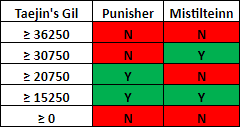
\includegraphics[width=9cm]{./Chapters/gil_pickups.png}
\endgroup

\pickup{Punisher}{forward and to the right if needed}
Push VH+T to the side.
\pickup{Particle Accelerator x6}{on the left side of the glass, then run backwards}
\pickup{Mistilteinn}{in of the long hallway if needed}
\pickup{Power Glove}{up the steps}
\vfill
\ 
\columnbreak
\begin{upgrade}
	\begin{itemize}
		\item Upgrade
		      \begin{itemize}
			      \item Accessories
			            \begin{itemize}
				            \item Power Glove
				                  \begin{itemize}
					                  \item Wicked Fang x41 (3x EXP)
					                  \item Particle Accelerator x6 (*)
				                  \end{itemize}
				            \item Goddess's Favor
				                  \begin{itemize}
					                  \item Particle Accelerator x1 (*)
				                  \end{itemize}
			            \end{itemize}
		      \end{itemize}
		\item Dismantle
		      \begin{itemize}
			      \item Accessories
			            \begin{itemize}
				            \item Goddess's Favor * (Scarletite, Perfume, Ribbon)
				            \item Ribbon (Dusklight Dew x6)
			            \end{itemize}
		      \end{itemize}
		\item Upgrade
		      \begin{itemize}
			      \item Warrior's Wristband * on Snow
			            \begin{itemize}
				            \item Scarletite (Power Glove Lv. 9)
			            \end{itemize}
		      \end{itemize}
	\end{itemize}
\end{upgrade}
	\begin{menu}
		\begin{itemize}
			\paradigm
			\begin{itemize}
				\item Battle Team
				      \begin{itemize}
					      \item Switch Sazh with Snow (1 $\leftrightarrow$ 2)
				      \end{itemize}
				\item \paradigmdeck{%
					      \paradigmline{Sazh}{Snow}{Vanille}}%
				      {\paradigmline{(\rav)}{\com}{\com}}%
				      {\paradigmline[2]{\textit{\com}}{\textit{\com}}{\textit{\com}}}%
				      {\paradigmline{(\rav)}{\sen}{(\rav)}}%
				      {\paradigmline{(\com)}{(\sen)}{\med}}%
				      {\paradigmline{\rav}{(\com)}{(\rav)}}%
				      {\paradigmline{\rav}{\rav}{\rav}}
			\end{itemize}
			\crystarium
			\begin{itemize}
				\item Sazh
				      \begin{itemize}
					      \item Commando
					            \begin{itemize}
						            \item 5 nodes, HP +70
					            \end{itemize}
				      \end{itemize}
				\item Snow
				      \begin{itemize}
					      \item Commando
					            \begin{itemize}
						            \item ($\downarrow$) 15 nodes, HP +30 end of stage 7
					            \end{itemize}
				      \end{itemize}
				\item Vanille
				      \begin{itemize}
					      \item Medic
					            \begin{itemize}
						            \item 1 left, Curaja
						            \item 1 Node, Role Level
					            \end{itemize}
				      \end{itemize}
			\end{itemize}
			\equip
			\begin{itemize}
				\item Snow
				      \begin{itemize}
					      \item WW Lv 8 $\rightarrow$ Power Glove *
				      \end{itemize}
				\item Vanille ($\rightarrow$)
				      \begin{itemize}
					      \item Shield Talisman $\rightarrow$ Black Belt *
				      \end{itemize}
			\end{itemize}
		\end{itemize}
	\end{menu}
Activate \textbf{Ethersol, Fortisol, Aegisol}.
\vfill
\renewcommand{\first}{[1] Aggression (\rav/\com/\com)}
\renewcommand{\second}{[2] Cerberus (\com/\com/\com)}
\renewcommand{\third}{[3] Mystic Tower (\rav/\sen/\rav)}
\renewcommand{\fourth}{[4] Solidarity (\com/\sen/\med)}
\renewcommand{\fifth}{[5] Relentless Assault (\rav/\com/\rav)}
\renewcommand{\sixth}{[6] Tri-Disaster (\rav/\rav/\rav)}
\begin{battle}[2:03]{Proudclad 2}
		\begin{itemize}
			\item \second
			      \begin{itemize}
				      \item Attack-Blitz, \rav-buffer the Blitz into
			      \end{itemize}
			\item \sixth
			      \begin{itemize}
				      \item Libra
				      \item Cold Blood
				      \item Shift towards the end of Cold Blood (as Sazh performs the second from last shot)
			      \end{itemize}
			\item \fifth
			      \begin{itemize}
				      \item Repeat
				      \item Shift as soon as Sazh starts shooting
			      \end{itemize}
			\item \first
			      \begin{itemize}
				      \item Cold Blood
				      \item Shift towards the end of Cold Blood (as Sazh performs the second from last shot)
			      \end{itemize}
			\item \second
			      \begin{itemize}
				      \item Renew
				      \item Until stagger runs out, Auto-battle 3 Attacks, alternate with Vanille to keep PC2 in the air
				      \item Attack-Attack-Blitz, \rav-buffer the Blitz
			      \end{itemize}
			\item \third
			      \begin{itemize}
				      \item Auto-chain one spell
				      \item \textit{Oneiric Maelstrom}:
				            \begin{itemize}
					            \item Renew to prevent Sazh from getting launched
					            \item Auto-chain 2 spells
					            \item Cold Blood
				            \end{itemize}
				      \item \textit{Muon Blaster $\rightarrow$ Oneiric Maelstrom}
				            \begin{itemize}
					            \item Renew to prevent Sazh from getting launched
					            \item Cold Blood
				            \end{itemize}
				      \item \textit{Muon Blaster $\rightarrow$ Muon Blaster}
				            \begin{itemize}
					            \item Cold Blood to prevent Sazh's interruption
				            \end{itemize}
				      \item Shift towards the end of Cold Blood, try to not let Snow do another Steelguard
			      \end{itemize}
			\item \fifth
			      \begin{itemize}
				      \item Repeat
				      \item Shift as soon as Sazh starts shooting
			      \end{itemize}
			\item \first
			      \begin{itemize}
				      \item Repeat
				      \item Shift towards the end of Cold Blood (as Sazh performs the second from last shot)
			      \end{itemize}
			\item \second
			      \begin{itemize}
				      \item Blitz-Blitz
				      \item Repeat
			      \end{itemize}
			\item \textit{If unlikely to kill before stagger ends}:
			      \begin{itemize}
				      \item \first
				            \begin{itemize}
					            \item Repeat and shift immediately
				            \end{itemize}
				      \item \second
				            \begin{itemize}
					            \item Hope and Cry
				            \end{itemize}
			      \end{itemize}
 					\item \textit{If Proudclad survives with low HP:}
					\begin{itemize}
						\item \second
							\begin{itemize}
								\item Repeat until victory, shift to [4] for heals
							\end{itemize}
							\end{itemize}
				     \item \textit{If Proudclad survives with high HP:}
					\begin{itemize}
						\item Blitz and \rav-buffer into
						\item \sixth
							\begin{itemize}
								\item Fire-Thunder-Fire-Thunder
								\item Repeat until \stagger
								\item If HP is still high, Cold Blood
							\end{itemize}
						\item \second
							\begin{itemize}
								\item Repeat until victory, shift to [4] for heals
							\end{itemize}
			      \end{itemize}
		\end{itemize}
\end{battle}
\save{1}
\vfill
\ 

\chapter[Chapter 13]{}
\begin{multicols}{2}
\begin{shop}{162\,000}
\begin{itemize}
    \item Eden Pharmaceuticals
    \begin{itemize}
        \item Sell
        \begin{itemize}
            \item Weapons: Everything
            \item Accessories: Everything but Warrior's Wristband
            \item Components: Everything
        \end{itemize}
        \item Buy
        \begin{itemize}
            \item Deceptisol x3
            \item Fortisol x3
            \item Aegisol x3
        \end{itemize}
    \end{itemize}
\end{itemize}
\end{shop}

\begin{menu}
\begin{itemize}
    \paradigm
    \begin{itemize}
        \item Battle Team
        \begin{itemize}
            \item Switch Sazh with Vanille (1 $\leftrightarrow$ 3)
        \end{itemize}
        \item Snow:
        \item \paradigmdeck{%
\paradigmline{Vanille}{Snow}{Sazh}}%
{\paradigmline{(\med)}{\com}{(\com)}}%
{\paradigmline{(\sab)}{\com}{\com}}%
{\paradigmline{(\sab)}{\sen}{(\syn)}}%
{\paradigmline{(\rav)}{(\rav)}{(\syn)}}%
{\paradigmline[5]{\textit{(\sab)}}{\textit{(\rav)}}{\textit{\rav}}}%
{\paradigmline{\rav}{\rav}{\rav}}
	\item Lightning:
        \item \paradigmdeck{%
\paradigmline{Vanille}{Snow}{Sazh}}%
{\paradigmline{(\rav)}{(\rav)}{(\syn)}}%
{\paradigmline{\rav}{\rav}{\rav}}
{\paradigmline{(\sab)}{\sen}{(\syn)}}%
{\paradigmline{(\sab)}{\com}{\com}}%
{\paradigmline{(\med)}{\com}{(\com)}}%
{\paradigmline[6]{\textit{(\sab)}}{\textit{(\rav)}}{\textit{\rav}}}
    \end{itemize}
    \crystarium
    \begin{itemize}
        \item Vanille
        \begin{itemize}
            \item Medic
            \begin{itemize}
            	\item 8 nodes Left 1, HP +100 to the side
            \end{itemize}
        \end{itemize}
        \item Snow
        \begin{itemize}
            \item Commando
            \begin{itemize}
                \item 16 nodes, Role level 4
            \end{itemize}
        \end{itemize}
        \item Sazh
        \begin{itemize}
            \item Commando
            \begin{itemize}
                \item 5 nodes up 2, Adrenaline to the top
                \item 3 nodes right 2, Accessory to the side
                \item 2 nodes, HP +100
            \end{itemize}
        \end{itemize}
    \end{itemize}
    \equip
    \begin{itemize}
        \item Sazh
        \begin{itemize}
            \item Optimize: Balanced
        \end{itemize}
    \end{itemize}
\end{itemize}
\end{menu}

Activate \textbf{Deceptisol} during the jump to the left, don't cancel.
Activate \textbf{Fortisol, Aegisol} before the statue.
\vfill


\renewcommand{\second}{[2]/[4] Devastation (\sab/\com/\com)}
\renewcommand{\fifth}{[5]/[6] Smart Bomb (\sab/\rav/\rav)}
\renewcommand{\sixth}{[6]/[2] Tri-Disaster (\rav/\rav/\rav)}
\begin{battle}{Bandersnatch \& Jabberwocky}
\begin{itemize}
    \item \fifth
    \begin{itemize}
        \item Imperil x5 Bandersnatch
        \item Repeat until Imperil is inflicted
    \end{itemize}
    \item \sixth
    \begin{itemize}
        \item Aerora-Fira Bandersnatch
        \begin{itemize}
            \item If only Vanille was knocked down, Aerora is enough
            \item If Bandersnatch reaches 410\%, drop everything and summon.
        \end{itemize}
        \item Repeat
        \item X - Gestalt
        %\item {\it If below 415\% chain:} (B - Force Blasters) x2
        \item {\it If below 485\% chain:} B - Force Blasters
        \item Y - Gaian Salvo
        \item Retry if not dead
        \item Auto-chain
        \item Shift after Snow's fifth Attack
    \end{itemize}
    \item \fifth
    \begin{itemize}
        \item If Breath of the Beast, shift to [3]/[1] until the attack is done
        \item Deprotect-Poison-Deprotect-Poison-Poison
        \item Cancel and repeat if the second Deprotect doesn't land
        \item Shift when Snow finishes his second string
    \end{itemize}
    \item \sixth
    \begin{itemize}
        \item Fire-Water-Aerora
        \item Auto-chain 2-3 spells for interruption
        \item Shift to cancel Snow's ready animation
    \end{itemize}
    \item \fifth
    \begin{itemize}
        \item Repeat \textit{if no Deprotect else } Poison x5
    \end{itemize}
    \item \second
    \begin{itemize}
        \item Repeat if no Deprotect, else Poison x5
        \item Repeat until victory
    \end{itemize}
\end{itemize}
\itemdrop{0.13}{Aegisol}
\end{battle}
\decep{while jumping}{back of the Megrim Thresher} If had 3 Deceptisols, skip the cancel.

\begin{menu}
\begin{itemize}
    \paradigm
    \begin{itemize}
        \item Set the third paradigm as default
    \end{itemize}
\end{itemize}
\end{menu}
\vfill
\newpage
Activate \textbf{Ethersol, Fortisol, Aegisol}.

\renewcommand{\second}{[2]/[4] Devastation (\sab/\com/\com)}
\renewcommand{\fifth}{[5]/[6] Smart Bomb (\sab/\rav/\rav)}
\renewcommand{\sixth}{[6]/[2] Tri-Disaster (\rav/\rav/\rav)}

\renewcommand{\third}{[3]/[3] Premeditation (\sab/\sen/\syn)}
\renewcommand{\first}{[1]/[5] Tireless Charge (\med/\com/\com)}

\begin{battle}{Wladislaus}
\begin{itemize}
    \item \third
    \begin{itemize}
        \item Libra
        \item Deprotect x5
        \item Shift after Sazh's third Enfire
    \end{itemize}
    \item \second
    \begin{itemize}
        \item If no Deprotect, Repeat
        \item Renew
        \item If no Deprotect, Repeat
        \item Repeat after Deprotect is removed via Mounting Contempt
    \end{itemize}
    \item \third
    \begin{itemize}
        \item If no Deprotect, Repeat
        \item Shift after Snow is hit by Mounting Contempt
    \end{itemize}
    \item \first
    \begin{itemize}
        \item Auto-heal
        \item Auto-heal after Wladislaus's attack
        \item Shift after Snow's fifth attack, cancel ready animation
    \end{itemize}
    \item \second
    \begin{itemize}
        \item Should die to Snow and Sazh. Otherwise repeat same process as above.
    \end{itemize}
\end{itemize}
\end{battle}

Take the left elevator, then \textbf{Ethersol} and \textbf{Deceptisol} while it rises. On the jumps, activate \textbf{Fortisol}, \textbf{Aegisol}, Menu.
\vfill
\begin{menu}
\begin{itemize}
        \begin{multicols}{2}
    \crystarium
    \begin{itemize}
        \item Sazh
        \begin{itemize}
            \item Commando
            \begin{itemize}
                \item 4 nodes, HP +90
            \end{itemize}
            \item Sentinel
            \begin{itemize}
                \item 6 nodes, Provoke
            \end{itemize}
        \end{itemize}
        \item Snow
        \begin{itemize}
            \item Commando
            \begin{itemize}
                \item 6 nodes, Str +30
            \end{itemize}
        \end{itemize}
        \item (Optional) Vanille
        \begin{itemize}
            \item Medic
            \begin{itemize}
                \item 3/6 nodes, HP +200 x2
            \end{itemize}
        \end{itemize}
    \end{itemize}
    \equip
    \begin{itemize}
        \item Snow
        \begin{itemize}
            \item Remove
            \begin{itemize}
                \item All Power Gloves
            \end{itemize}
        \end{itemize}
        \item Sazh
        \begin{itemize}
            \item Optimize: Balanced
        \end{itemize}
        \item Snow
        \begin{itemize}
            \item Optimize: Balanced
        \end{itemize}
    \end{itemize}
\end{multicols}
    \paradigm
    \begin{itemize}
        \item Battle Team
        \begin{itemize}
            \item Switch Vanille with Sazh (1 $\leftrightarrow$ 3)
        \end{itemize}
        \end{itemize}
        \begin{center}Snow\end{center}
        
        \paradigmdeck{%
\paradigmline{Sazh}{Snow}{Vanille}}%
{\paradigmline{\com}{\com}{\med}}%
{\paradigmline[2]{\textit{\com}}{\textit{\com}}{\textit{(\rav)}}}%
{\paradigmline{(\sen)}{\sen}{(\med)}}%
{\paradigmline{\syn}{\rav}{\rav}}%
{\paradigmline{\rav}{\rav}{\sab}}%
{\paradigmline{\rav}{\rav}{\rav}}


	\begin{center}Lightning\end{center}
	
        \paradigmdeck{%
\paradigmline{Sazh}{Snow}{Vanille}}%
{\paradigmline{\syn}{\rav}{\rav}}%
{\paradigmline{\rav}{\rav}{\rav}}	%
{\paradigmline{(\sen)}{\sen}{(\med)}}%
{\paradigmline[4]{\textit{\com}}{\textit{\com}}{\textit{(\rav)}}}%
{\paradigmline{\com}{\com}{\med}}%
{\paradigmline{\rav}{\rav}{\sab}}
\end{itemize}

\end{menu}
\renewcommand{\first}{[1]/[5] Tireless Charge ((\com)/\com/\med)}
\renewcommand{\second}{[2]/[4] Aggression (\com/\com/\rav)}
\renewcommand{\third}{[3]/[3] Consolidation (\sen/\sen/\med)}
\renewcommand{\fourth}{[4]/[1] Malevolence (\syn/(\rav)/\rav)}
\renewcommand{\fifth}{[5]/[6] Smart Bomb (\rav/\rav/\sab)}
\renewcommand{\sixth}{[6]/[2] Tri-Disaster (\rav/\rav/\rav)}
\begin{battle}{Tiamat Eliminator}
\begin{itemize}
    \item \second
    \begin{itemize}
        \item Attack-Attack-Blitz, \rav-buffer the Blitz
    \end{itemize}
    \item \sixth
    \begin{itemize}
        \item Cold Blood
        \item Libra
        \item Auto-chain if Tail Hammer
        \item Repeat just before Stagger, shift after Sazh fires the first bullet
    \end{itemize}
    \item \fourth
    \begin{itemize}
        \item Shift
    \end{itemize}
    \item \sixth
    \begin{itemize}
        \item Repeat
    \end{itemize}
    \item \second
    \begin{itemize}
        \item Blitz-Blitz
        \item Repeat, ATB refresh with [1] until stagger ends
        \item Attack-Attack-Blitz when Tiamat drops to the ground, \rav-buffer the Blitz
    \end{itemize}
    \item \fifth
    \begin{itemize}
        \item Repeat until stagger, refresh with [6]
        \item Renew if Pinpoint Beam
        \item Shift to [6] if Imperil and Deprotect
    \end{itemize}
    \item \second
    \begin{itemize}
        \item Blitz-Blitz
        \item Repeat until Victory
    \end{itemize}
\end{itemize}
\end{battle}

\begin{shop}{44\,000}
\begin{itemize}
    \item Eden Pharmaceuticals
    \begin{itemize}
        \item Sell
        \begin{itemize}
            \item Accessories
            \begin{itemize}
                \item Imperial Armlet
            \end{itemize}
        \end{itemize}
        \item Buy
        \begin{itemize}
            \item Librascope x2
            \item Fortisol x1
            \item Aegisol x1
        \end{itemize}
    \end{itemize}
\end{itemize}
\end{shop}
\end{multicols}
\pickup{Ethersol}{in the final hallway}
Activate all shrouds.
\renewcommand{\first}{[1]/[5] Tireless Charge (\com)/\com/\med)}
\renewcommand{\second}{[2]/[4] Aggression (\com/\com/\rav)}
\renewcommand{\third}{[3]/[3] Consolidation (\sen/\sen/\med)}
\renewcommand{\fourth}{[4]/[1] Malevolence (\syn/(\rav)/\rav)}
\renewcommand{\fifth}{[5]/[6] Smart Bomb (\rav/\rav/\sab)}
\renewcommand{\sixth}{[6]/[2] Tri-Disaster (\rav/\rav/\rav)}

\begin{battle}{Barthandelus 3}
\begin{multicols}{2}
\begin{itemize}
    \item \second
    \begin{itemize}
        \item Librascope
        \item Attack-Blitz, \rav-buffer the Blitz
    \end{itemize}
    \item \fifth
    \begin{itemize}
        \item Fire-Thunder-Fire-Thunder
        \item Repeat
        \item Repeat two spells if no Imperil or was inflicted late
        \item Shift at 200\% chain (no Imperil) or 220\% chain (Imperil)
    \end{itemize}
    \item \third
    \begin{itemize}
        \item Potion twice
        \item \textit{If no Imperil}
        \begin{itemize}
            \item Potion
            \item Shift after Ultima
            \item \fifth
            \begin{itemize}
                \item Throw Potions until Imperil inflicts
                \item If \stagger\ Retry
            \end{itemize}
            \item \first
            \begin{itemize}
                \item Repeat until Ultima
            \end{itemize}
            \item \third
            \begin{itemize}
                \item Potions
                \item Shift after Ultima hits
            \end{itemize}
        \end{itemize}
        \item \textit{If Imperil and no Deprotect}
        \begin{itemize}
            \item \fifth
            \begin{itemize}
                \item Renew
                \item Shift after Deprotect
            \end{itemize}
        \end{itemize}
    \end{itemize}
    \item \sixth
    \begin{itemize}
        \item Renew if anyone is yellow health
        \item Cold Blood
        \item Shift towards the end for ATB refresh
    \end{itemize}
    \item \second
    \begin{itemize}
        \item Blitz-Blitz
        \item Repeat. Shifter after Snow jumps back.
    \end{itemize}
    \item \first
    \begin{itemize}
        \item Repeat
        \item Repeat after Laughter, try to get one in during Laughter
        \item ATB refresh if possible
    \end{itemize}
    \item \second
    \begin{itemize}
        \item Repeat until victory or stagger end
    \end{itemize}
    \columnbreak
    \item \textit{If stagger ends}:
    \item \third
    \begin{itemize}
        \item Renew
        \item Potion after Ultima
    \end{itemize}
    \item \textit{If Bart is close to death}:
    \begin{itemize}
        \item \first
        \begin{itemize}
            \item Repeat until victory
        \end{itemize}
    \end{itemize}
    \item \textit{Else}:
    \begin{itemize}
        \item \sixth
            \begin{itemize}
                \item Fire-Thunder-Fire-Thunder
                \item Repeat until \stagger
                \item Use [5] to inflict any missing debuffs
            \end{itemize}
        \item \first
        \begin{itemize}
            \item Repeat until victory
        \end{itemize}
    \end{itemize}
\end{itemize}
\end{multicols}
\end{battle}
\begin{battle}{Orphan 1}
\begin{multicols}{2}
\begin{itemize}
    \item \second
    \begin{itemize}
        \item Summon, Shift immediately
    \end{itemize}
    \item \fourth
    \begin{itemize}
        \item \textbf{MERCILESS JUDGMENT}
        \item Haste-Vigilence Sazh
        \item Repeat Snow
        \item Shift to Cancel Snow's Animation
    \end{itemize}
    \item \third
    \begin{itemize}
    	\item \textbf{SLAP}, Shift after Challenge Lands
    \end{itemize}
    \item \fourth
    \begin{itemize}
        \item Auto-support Vanille (Haste)
        \item Bravery-Enthunder Sazh
        \item Librascope
        \item Shift to tank slap
    \end{itemize}
    \item \third
    \begin{itemize}
        \item \textbf{SLAP}, Shift after Challenge lands
    \end{itemize}
    \item \fourth
    \begin{itemize}
        \item Repeat Snow
    \end{itemize}
    \item \fifth
    \begin{itemize}
        \item Fire-Thunder-Fire-Thunder
        \item Shift to tank next attack
    \end{itemize}
    \item \third
    \begin{itemize}
        \item \textbf{SLAP/REQUIEM}, Shift after Challenge lands
    \end{itemize}
    \item \fifth
    \begin{itemize}
    	  \item Repeat
    	  \item Renew
    \end{itemize}
    \vfill\null
    \columnbreak
    \item From now until Tireless Charge, shift to [3] whenever Orphan attacks and shift back after re-provoke
    \item \fifth
    \begin{itemize}
        \item Repeat or use Potions until Deprotect, Imperil, Poison
        \item Tank in [3]
        \item After \stagger use Cold Blood
        \item Shift after all 3 debuffs have landed and used Cold Blood
    \end{itemize}
    \item \first
    \begin{itemize}
        \item Repeat until \textbf{Merciless Judgement}
        \item Phoenix Down Vanille if needed
        \item \textbf{MERCILESS JUDGMENT}
        \item \textbf{OPPOSITE EXTREMES}
        \item Elixir, if locked into Blitz buffer into [6] and Elixir there
        \item Repeat a Blitz and \rav-buffer
    \end{itemize}
    \item \sixth
    \begin{itemize}
        \item Fire-Thunder-Fire-Thunder
    \end{itemize}
    \item \fourth
    \begin{itemize}
        \item Renew, Haste Sazh, depend order depending on if Sazh was hit
    \end{itemize}
    \item \textit{If Orphan uses Vile Exploitation}:
    \begin{itemize}
        \item Repeat while Sazh is still healthy
        \item Summon
    \end{itemize}
    \item \textit{If Orphan uses Dies Irae or Progenitorial Wrath}:
    \begin{itemize}
        \item Summon, execute when the hand swings up
    \end{itemize}
    \item \first
    \begin{itemize}
        \item Blitz-Blitz
        \item Repeat with ATB refresh with [2] until victory
        \item Gestalt mode to poison stall to kill if things go sideways
    \end{itemize}
\end{itemize}
\end{multicols}
\end{battle}
\begin{battle}{Orphan 2}
\begin{multicols}{2}
\begin{itemize}
    \item \second
    \begin{itemize}
        \item Single Blitz, trigger early
	\item Shift when camera focuses on Orphan
    \end{itemize}
    \item \fourth
    \begin{itemize}
        \item Auto-support Vanille (Down, Haste)
        \item Auto-support Sazh (Haste)
        \item Auto-support Snow (Haste)
	\item Shift after Snow's fifth spell
    \end{itemize}
    \item \sixth
    \begin{itemize}
        \item Auto-chain/Fire-Thunder-Fire-Thunder
    \end{itemize}
    \item \fourth
    \begin{itemize}
        \item Enthunder Snow
        \item If Slap, try to use Potion or Renew to not get launched
        \item Enthunder-Bravery Sazh
        \item Shift after Snow's fifth spell
    \end{itemize}
    \columnbreak
    \item \fifth
    \begin{itemize}
        \item Repeat until \stagger
        \item Aerora-Aero
        \item Repeat until Deprotect and Imperil
	\item Renew if necessary/possible
    \end{itemize}
    \item \first
    \begin{itemize}
        \item Blitz-Blitz if in Blitz Range
        \item Auto-battle single attack if just Launched
        \item Cancel second Blitz to make sure that they land after landing if needed
        \item Repeat until victory
    \end{itemize}
\end{itemize}
\end{multicols}
\end{battle}


\end{document}
